\iffalse

{\bf FIVE parts of the writing}
\begin{enumerate}
\item {Reading and review related works - papers and their references.}
\item {Elaborating some particular terminologies - wikipedia}
\item {Writing our own algorithms - leave out figure making}
\item {Performance evaluations - refer to review paper on HOW-TO}
\item {Making figures for illustrating our own algorithms}
\end{enumerate}

\newpage

\section{Defense Input}

*. Clarify what is manually, what is automatically implemented.
*. Symmetry computation, automatically or manually?
*. How to determine whether we are requiring for tapering computation.
*. The 3rd important parameter, \tau_\delta, which is used to control projection.
*. Add how to handle follow-me in the future work.
*. Incorporate changes from 3DPVT, defense and TVCG.

%%%%% To-Do list %%%%%
aim to tvcg | but target at SIGGRAPH

* keyslice detection survey on curve comparison.

* in intro, add recently 2 years of related work.
* survey CVPR, SIGGRAPH, papers for comparison
%%%%% to do list %%%%%
\newchapt{TODO}{chapt}{TODO}
DOING  Add the rendering results, including google earth?

\section{Appendix}
%% mathematic morphological operation: close/open/dilation/erosion.
%% 3D computational geometry.
%% kd tree introduction on point-based construction and query
%% double check scan-line polygon filling algorithm

\section{Reference}

%% similarity measurement.
%% point cloud segmentation.
%% window detection.
%% dilation, erosion on binary image.

\newpage
\fi % \iffalse

%%%%% New Chapter %%%%%
%%%%% New Chapter %%%%%
\newchapt{Introduction}{chapt_intro}{Introduction}

The 3D modeling of urban buildings is an area of active research
with increasing attention drawn from the computer graphics and
computer vision communities.
A survey by Tang {\it et al.} offers a good overview of the current
status of research and techniques used for building information modeling \cite{RW_THALL}.
Current state-of-the-art algorithms include procedural modeling,
3D laser scanning, and image-based approaches.
In addition, conventional modeling tools are commonly used for this purpose.
The most accurate input source for modeling {\it existing} buildings, though,
remains laser range scanners \cite{RDP_BR}.
They provide high geometric detail by collecting range data from hundreds
of meters away with an accuracy on the order of a few millimeters \cite{RDP_LRS}.
This fidelity is appropriate for construction, architecture, cultural
heritage, and forensics applications.
Unfortunately, laser range scanning can produce an overwhelming amount of data,
which poses great challenges to visualization software that require lightweight
3D models for interactive use.
Polygonal data generated from range scans are therefore too dense for use in
web-based applications such as Google Earth \cite{RDP_GOOGE} and Microsoft Virtual Earth
\cite{RDP_MSE}.
These applications work best with lightweight models consisting of only
hundreds of polygons.

The goal of this work is to produce high-quality lightweight models of
urban buildings from large-scale 3D range data in a semi-automatic way.
The proposed solution is inspired by the simple paradigm embedded in
procedural modeling as well as interactive tools such as Google SketchUp.
The core of these methods is that a simple set of extrusion and tapering
operations applied to 2D contours can grow a wide array of complex 3D urban models.
We propose a reverse engineering approach to infer key cross-sectional
planar contours along with a set of extrusion and tapering operations to derive
lightweight models that conform to the 3D range data.

The main contribution of this work is that it provides a framework for
lightweight modeling of urban buildings from heavy 3D point cloud datasets (PCD)
based on a series of extrusion and tapering operations along dominated axes.
The proposed framework combines the benefits of
\emph{a priori} knowledge of urban buildings and fast 2D image
processing techniques to perform 3D modeling of urban buildings
and can generate models across a wide spectrum of resolutions.
This offers the benefit of a cost-effective geometry compression
approach for voluminous range data within the domain of urban structures.
A particularly useful feature of the algorithm is that it outperforms
existing approximation techniques by preserving the sharpness of the raw
data, even at low resolution.
It can be applied to boost web-based 3D applications, virtual city touring,
and online gaming.

\section{Related Work}

In an attempt to steer clear of tedious and expensive hand-made models,
procedural modeling of buildings in \cite{PMB_MWH,PMB_WWS,PMB_PM} has been proposed.
By using an effective description language, buildings and streets of a virtual
city can be generated automatically.
The strength of this approach is that the description language can generate
a huge number of buildings and streets quickly and beautifully.
This is particularly useful for gaming and other computer graphics applications.
However, since the parameters used to generate the buildings are randomly
generated, the city generated with these buildings and streets is a virtual one.
This approach is not useful for attempting to model an {\it existing} building.
In order to do so, one has to manually specify the parameters of the building,
which is very cumbersome.
Our goal is to automatically infer the contours and extrusion/tapering parameters
of an existing building directly from dense range data.

Reconstruction of 3D models from range data has been addressed in
\cite{RE_Fisher,RE_CLF,RE_CD} with applications in numerous research areas,
including computer-aided design (CAD), computer vision, architectural modeling,
and medical image processing.
The authors in \cite{Okorn10} use a histogram of height data to detect floors
and ceilings for creating accurate floor plan models of building interiors.
In \cite{DP_OWYC}, the authors proposed a 3D building reconstruction from a
2D floor plan image.
With the help of a 2D floor plan image, both the interior and exterior of a
building can be reconstructed accordingly.
A survey on methods for generating 3D building models from architectural
floor plans is given in \cite{YIN09}.
However, reliance on 2D floor plans makes these approaches too limiting for
most applications, including our project.
In \cite{RE_TOGSH}, known manufacturing features were used to infer the
3D structure of mechanical parts.
Their method benefits from the domain knowledge that most of the mechanical
parts consist of predefined structures, such as holes, bosses, and grooves.
Our work is partially motivated by this idea since it also incorporates
{\it a priori} knowledge about the construction of urban buildings for further
inference.
However, their method is based on predefined simple geometry structures and
the assumption that the input 3D data has no holes.
This hinders their approach for those applications with incomplete data.

Medical image processing techniques are usually dealing
with low Signal-to-Noise Ratio (SNR) data.
There has been a lot of work on the medical 3D image reconstruction as in
\cite{MIR_BMMNB, MIR_KL, MIR_SKJ, MIR_SMHC, MIR_BVC}.
The basic ideas behind these approaches
are 3D reconstruction from sliced or histologic images using interpolation techniques.
The statistical inference are also intensively used to infer the low SNR images.
In \cite{MIR_FJS}, Sigworth tried to deal with low SNR image data
using maximum likelihood approach.
Because most of the statistical processes are computational intensity,
these approaches usually are heavy-duty approaches
in order to obtain accurate, high resolution models.

Multi-modal data fusion is another approach for large-scale urban environment modeling
where the LIght Detection And Ranging (LIDAR) scans are widely used \cite{UM_HYN}.
In \cite{UM_Zakhor}, both air and ground data are fused,
where LIDAR scans are used to create the models
and the camera images are used for texture mapping.
Citing the cumbersome and expensive use of laser scanners, the researchers
in \cite{AKBARZADEH06} propose an approach that relies solely on passive
sensors (cameras) mounted on a moving vehicle.
Dense 3D point cloud measurements are derived using their multi-view stereo
module based on multiple plane sweeping directions.
In an attempt to compress the voluminous data produced in the method of
\cite{AKBARZADEH06},
Xiao {\it et al.} introduced an approach for modeling facades along a street
using {\it a priori} knowledge about the buildings based on images \cite{UM_XFTQ}.
They achieve geometry compression and deliver a clean approximation of the
facades by applying a combination of plane fitting and window detection.
However, their automatic depth reconstruction techniques based on images may fail
when modeling highly reflective mirror-like buildings.

Toshev {\it et al.} proposed grammar based method for detecting and parsing
buildings from unorganized street-level point clouds \cite{RW_TMT} .
Despite its efficiency on modeling, the results could not generate
enough level of details for the buildings.
For example, the windows and doors are missing in the final models.
The same situation appears in \cite{RW_HDP}, where only building footprints
are extracted from the range data.
Johnston and Zakhor developed a method to generate
interior building floor plans from the exterior of the structure \cite{RW_JZ}.
They use a laser scanner to measure the range of
hundreds of thousands of points on interior walls of the building,
exploiting the fact that the laser can go through unobstructed windows.
The issue is when there are obstructed windows or many objects behind the windows,
the inferred floor plans become much less accurate.
Vanegas {\it et al.} presented a work that examines the changes in
building geometry from principle directions and reconstructs the models
using Manhattan-World grammars \cite{RW_VAB}.
This work produces models with much higher resolutions from
multiple calibrated aerial images, instead of 3D point clouds.
However, this method is not able to model tapered structures
which exist widely in buildings and can be handled by our approach.

The ball-pivoting algorithm (BPA) is an efficient technique
for meshing 3D point clouds to produce polygonal models \cite{BPA_BMRS}.
The generated meshes, however, constitute heavyweight models,
with the number of vertices nearly approaching the number of points in the
3D point cloud.
This limits its usefulness for web-based applications.
Although a BPA model can be simplified using approximation techniques such as
{\it qslim} \cite{BPA_GH},
the sharp detail of the original model is not preserved.
Recently, Sareen {\it et al.} proposed a contour based 3D point cloud
simplification approach for modeling free-form surface \cite{RW_SKC}.
The authors first extracted 2D slices from equally spaced slabs of point clouds.
In the second stage, a cubic B-spline curve is used to approximate
each 2D slice with the number of control points predefined by users.
The proposed method was applied to a facial scan data with 50k
data points and can achieve 5-20\% of overall size reduction ratio.
This is not scalable enough for point clouds of urban buildings which usually
consist of millions of data points and require much more size reduction ratio.


Simplification of 3D buildings is also an active research topic in
laser scanning research community \cite{LS_GAL,WDD_BBH,LS_BH}.
Gonzalvez {\it et al.} proposed an automatic approach to convert
a laser scanner point cloud into a realistic 3D polygonal model \cite{LS_GAL}.
They first segmented the unstructured point cloud into sections
based on vertical walls which are the
mainly characteristic of the shapes of the buildings.
Afterwards, sections and profiles are simplified automatically
based on Douglas-Peucker algorithm followed by a clustering process
which groups all related sections to extract partial primitives.
Finally, a growing clustering of each partial primitive is conducted
to obtain a global primitive.
The main issues in their method is that a number of thresholds
 have to be tested by the user before obtaining good results,
and the underlying building must be linear
in order to apply the proposed approach.

In addition to the aforementioned research projects carried on in academia,
some commercial products are developed in start-up companies.
In \cite{IND_YC}, the buildings in Manhattan are modeled to enhance
the virtual reality of social network.
The buildings are accurately modeled via aerial LIDAR data
and were associated with address and related social information.
Another commercial product is EdgeWise\textsuperscript{\texttrademark},
a new developed product by ClearEdge\textsuperscript{3D} \cite{IND_EW}.
They first apply ground extraction to classify the point cloud data.
And then the polygons are inferred for each classified data points
and are exported to be edited in Google SketchUp.
Essentially, this commercial tool only provides
a good starting point for interactive editing.

%%% the difference between our work and others.

%%%%%%%%%%%%%%%%%%%%%%%%%%%%%%%%
%%%%%%   Overview  %%%%%%%%
%%%%%%%%%%%%%%%%%%%%%%%%%%%%%%%%
\section{Overview}

We propose an efficient way to reconstruct 3D models from range data by
partitioning the data into thin cross-sectional volumetric slabs.
For each slab, all range data in that slab is projected onto a 2D
cross-sectional contour slice.
Producing this array of slices permits us to avoid costly computation directly
on 3D data.
A similarity measure is used to
cluster the sliced images together into {\it keyslices}.
This term is analogous to the use of ``keyframes'' in computer animation,
which denotes important snapshots in the animation sequence from which
intermediate results can be derived.
In essence, each keyframe is a slice in the spatiotemporal volume of
an animation.
Similarly, each keyslice is a 2D image which contains a {\it transitional}
cross-section of the building, encapsulating major contours in the facade.
The model is then generated by applying basic extrusion and tapering
operations from one keyslice to the next.
This produces a lightweight representation consisting of only a few
hundred polygons.

\begin{figure}[htbp]
\begin{center}
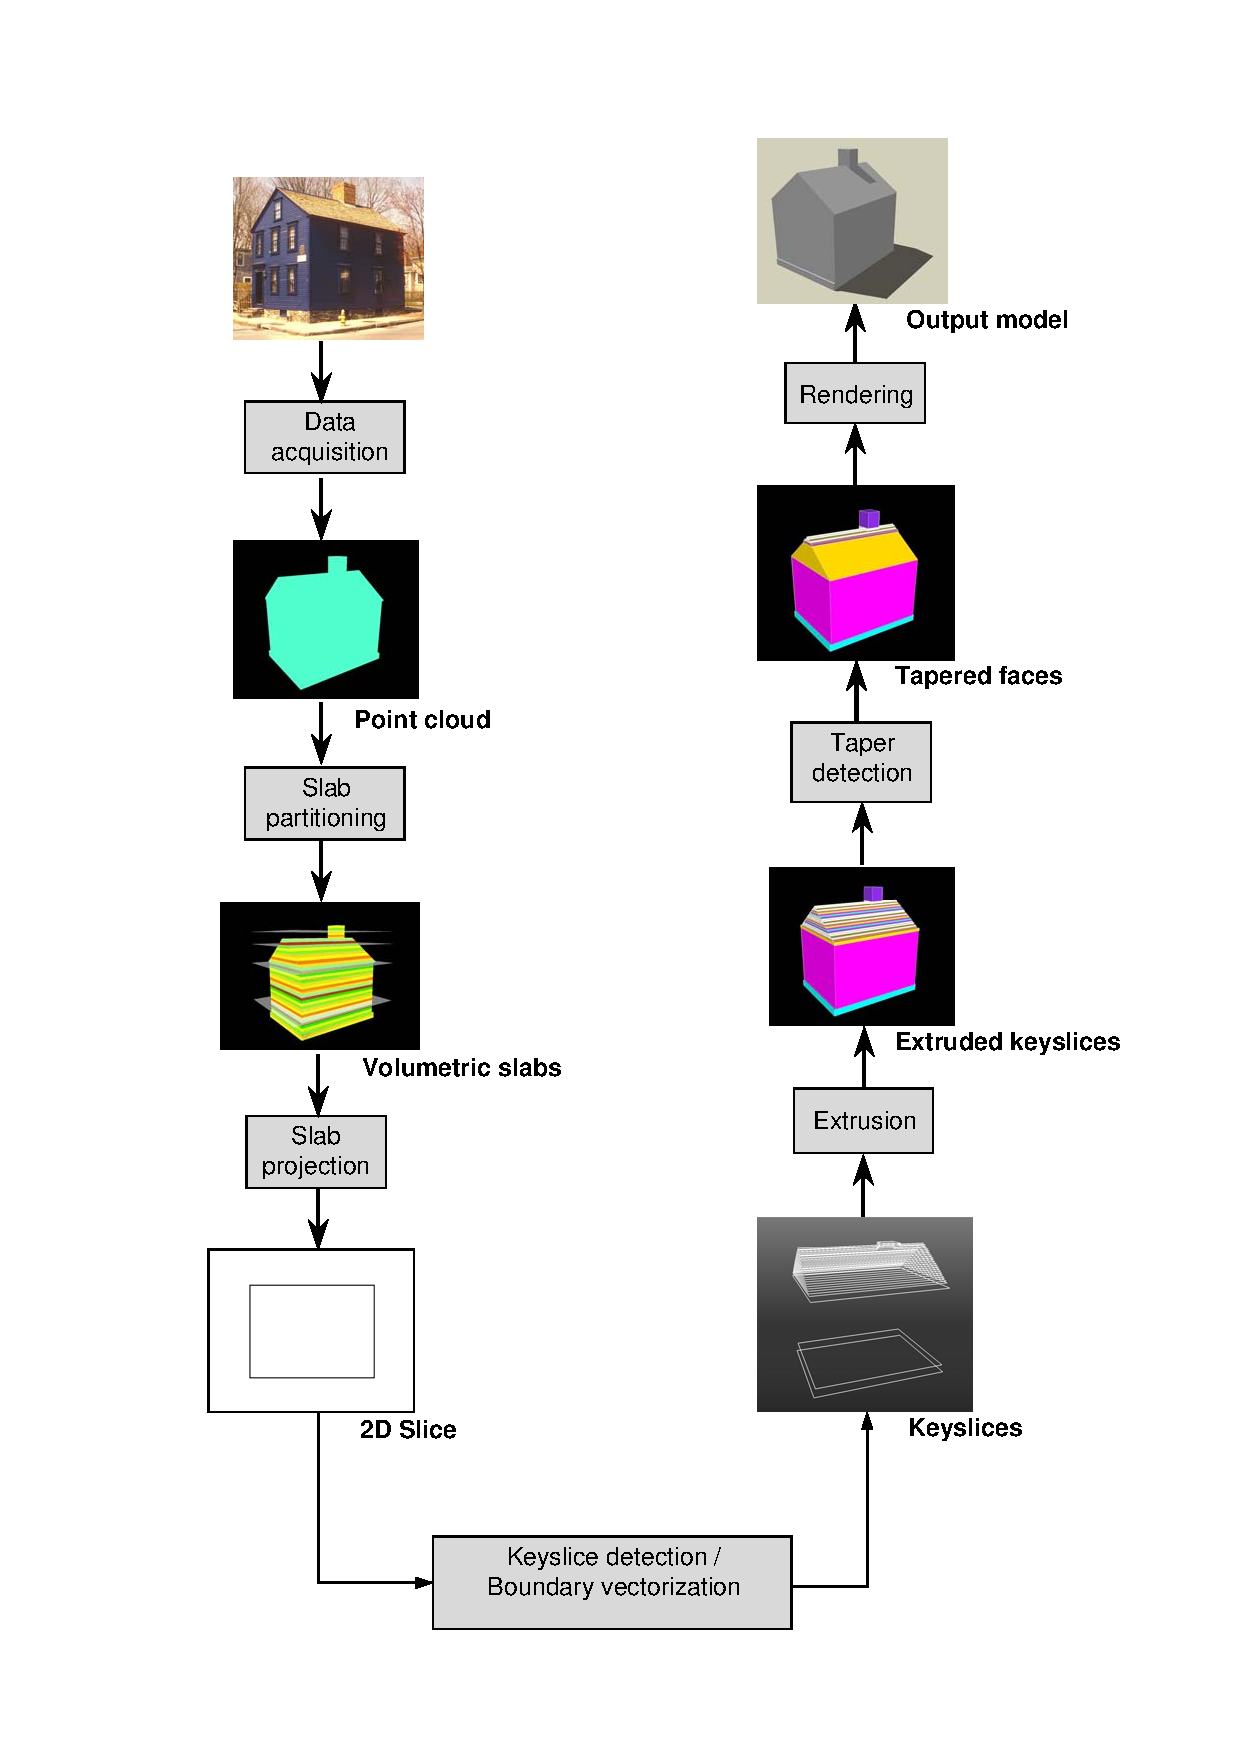
\includegraphics[width=.8\textwidth]{overview_new_vert.pdf}
\end{center}
\caption{Overview of the proposed approach.}
\label{fig:ov}
\end{figure}

An overview of our approach, depicted in \Fig{ov}, begins with the
acquisition of a dense 3D point cloud $C$ of a building.
$C$ is then partitioned into a non-overlapping set of volumetric slabs.
Each slab $S$ is associated with one projection plane $P$,
sitting at the base of $S$.
The purpose of partitioning $C$ is to establish a set of cross-sections,
or contour slices.
By examining the changes among these slices, we can identify the prominent
slices, or {\it keyslices} $K$, as well as the necessary extrusion and
tapering operations that must apply to them to generate the model.
By casting this 3D modeling task into a series of 2D operations, we
reduce the dimension of the problem to achieve a significant savings in
computational complexity.
Boundary vectorization are then carried out to these raster images $K$
to obtain the contours $T$.
After applying the extrusion and tapering operations on $T$,
the final model can be generated and rendered for visualization.

The modular flow diagram for our system is shown in \Fig{flow}.
The whole system consists of three stages of computation.
The first stage mainly contains pre-processing modules.
In this stage, 3D synthetic datasets are generated and
3D real datasets are obtained as input to the whole system.
Major plane detection is carried out to compute the normals of the major facades
for extracting 2D slices which are then enhanced by noise removal and
hole filling.
These enhanced 2D slices are then segmented for further processing.
The second stage is iteratively applied to each segment computed in
the first stage and plays key role for model reconstruction.
First, both distance measurement based and curvature based keyslice
detection are conducted in the keyslice detection module
to locate those prominent slices for the current segment.
Following this, boundary vectorization is carried out on these raster keyslices
to obtain the contours for reconstruction.
Furthermore, linear tapered structure is computed to reduce the model size.
The final stage is to model the range data
based on information computed in previous stages.
In model generation module, each segment is reconstructed by applying the extrusion
and tapering operations on the keyslice contours.
These models are then assembled in the module of model merging.
Finally, if exist, windows and doors are projected to generate the whole model.

\begin{figure}[htbp]
  \centering
  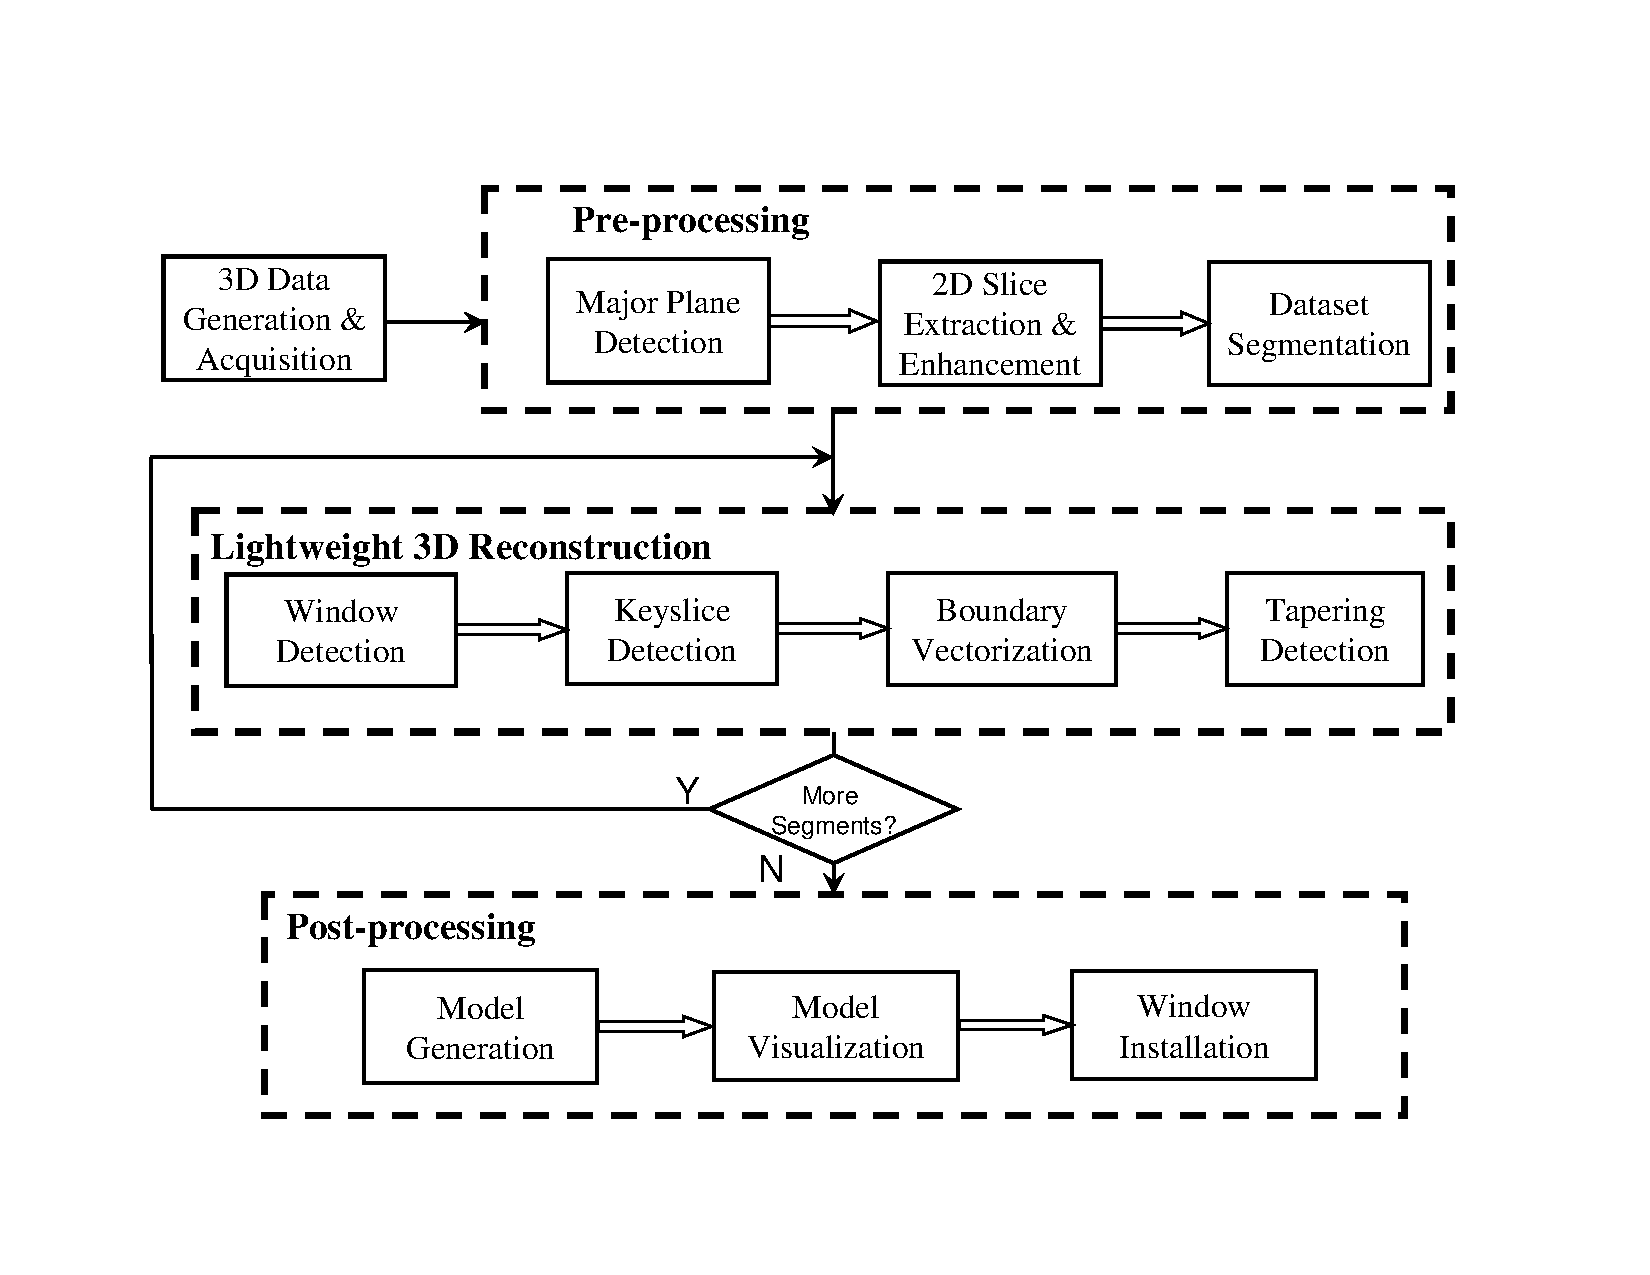
\includegraphics[width=\textwidth]{flow.pdf}
      \caption{Flow graph for proposed approach.}
      \label{fig:flow}
\end{figure}

The point cloud datasets in our experiments consist of synthetic and real ones.
The synthetic datasets are generated from 3D building models
with no noise introduced
and are used for proof of concept.
These 3D building models which were downloaded from Google SketchUp 3D warehouse
contain 3D faces and their normals.
Because we have the ground truth of reconstructed models,
that is, the original models,
the synthetic datasets can also be used to check the correctness and
measure the errors for reconstructed models.
On the other hand, the real datasets are acquired from laser scanners.
Due to the nature of buildings (with windows, doors) and blocking, the real
datasets also contain all kind of noise
and they are only used to validate the proposed approach.

\section{Synthetic Data Generation}

% Algorithm:
% transform 3D faces to 2D images using a matrix T.
% based on sampling rate, apply polygon filling on the 2D polygon, which handles concave polygons.
% special cases:
%      1. windows
%      2. hidden faces?
% transform sampled data back to 3D inv(T)

% Writing:
% the transformation matrix written in the rectification section.
% Appendix: polygon filling.

For a Google SketchUp building model, it needs to be exploded to decompose
any grouped faces.
This ensures each individual face of the model can be accessed.
We wrote a Ruby script using SketchUp APIs to dump all faces
and their normals into a file as input for point cloud dataset generation.
All faces laying on the same plane are marked, which is an important
information for correct data generation.

% some key APIs are ..... describe how to download the faces.

\begin{figure}[htbp]
\begin{center}
\begin{tabular}{c}
	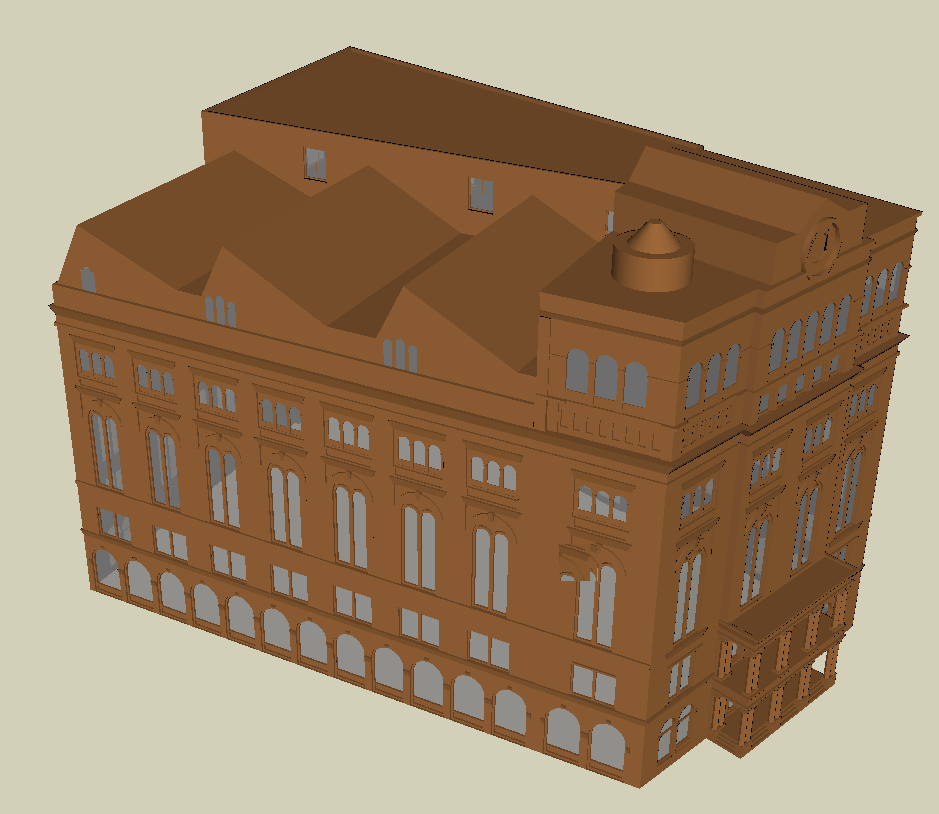
\includegraphics[width=0.4\textwidth]{cu_1.png} \\
	(a) \\
        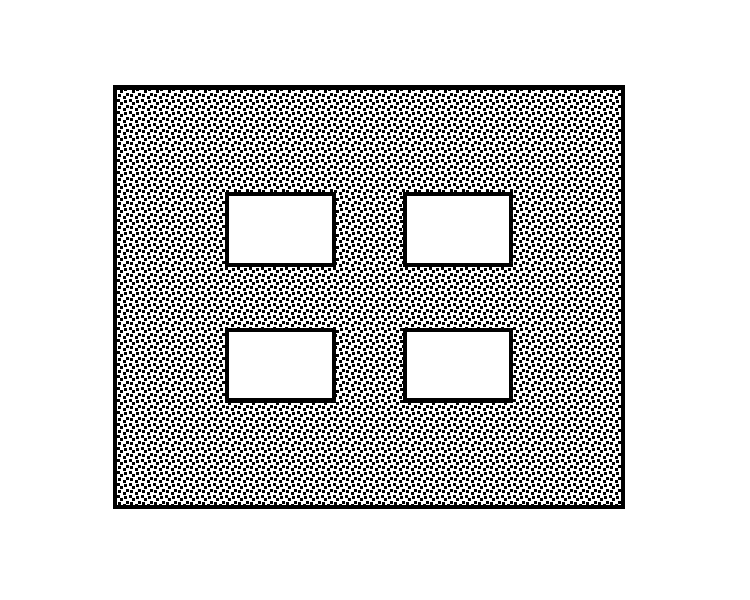
\includegraphics[width=0.4\textwidth]{sampling_face.pdf} \\
	(b) \\
	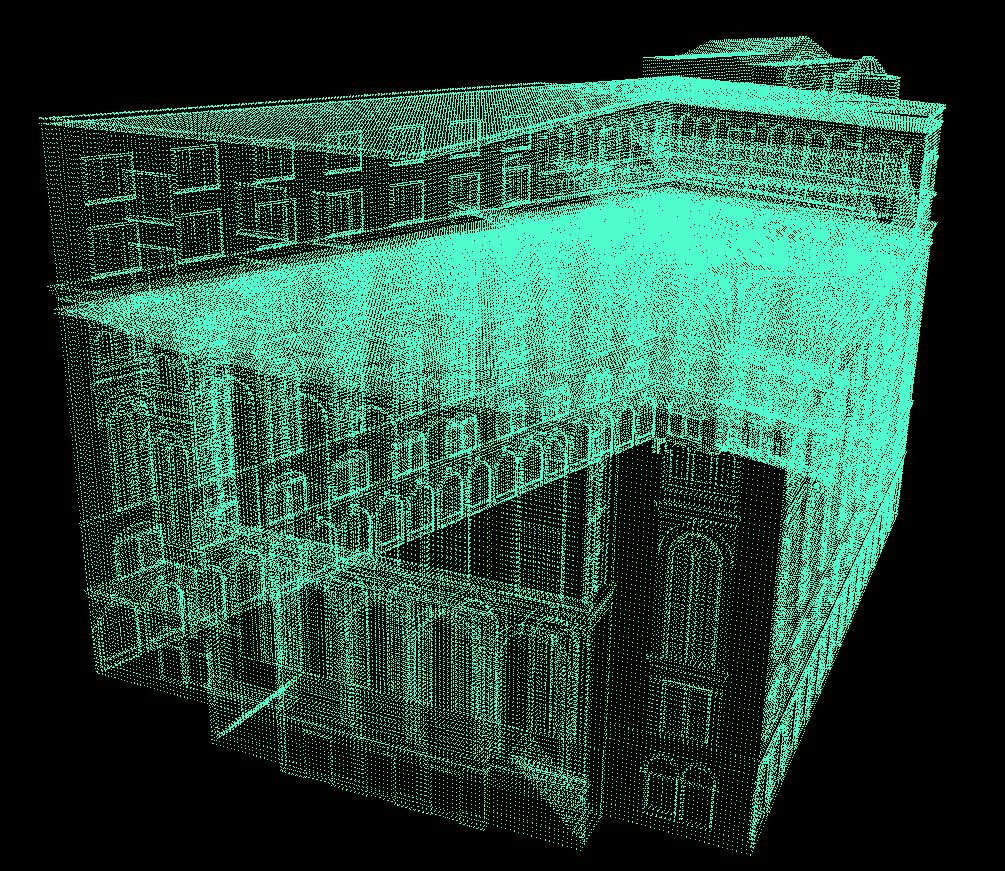
\includegraphics[width=0.4\textwidth]{cu_2.png} \\
	(c)
\end{tabular}
\end{center}
\caption{
The synthetic point cloud generation:
(a) the snapshot of a 3D model;
(b) the example of the sampling for embedded faces;
(c) the snapshot of the synthetic 3D point cloud from (a).
}
\label{fig:syn_data}
\end{figure}

With these faces and their normals,
 we can carry out the synthetic 3D point cloud data generation directly.
Alternatively, we can transform each 3D plane to 2D space, and then
transform those sampled data generated on 2D space back to 3D space.
To simplify the process, the co-planar 3D faces are first transformed onto a 2D plane.
Let ${\bf V} = \{v_0, v_1, ... v_i, ..., v_0\}$ be the set of vertices for a 3D face.
Let ${\bf F}$ be the set of faces sitting on the same plane.
Let $N_v$ be the normal of the plane and $|N_v| = 1$.
${\bf V, F }$ and $N_v$ are known from the SketchUp model and are input for the process.
We can construct another vector on the face, say $N_p = \overline{v_0v_1}$ and
normalize the vector $|N_p| = 1$, $N_p$ and $N_v$ are perpendicular to each other.
Let $N_s = N_p \times N_v$, that is, the cross product of the $N_p$ and $N_v$.
The transform matrix $M = [N_p, N_v, N_s]^T$ transforms the 3D vector
onto an 2D plane of the coordinate system with the axis $N_p, N_v,$ and $N_s$.

The remaining data generation process is similar to
the scan line based polygon filling.
A parameter $s$ is used to control the distance
between scan lines and to define the interval
between two consecutive synthetic data points.
For each scan line, we count the number of intersection points, $n$,
between the scan line and the face edges.
When $n$ is an odd number,
it starts to add points on scan line with the interval $s$.
For example, assume the current scan line is $y = 8$
and $(2, 8)$ is a new generated synthetic data point.
With the parameter $s = 4$, the next data point is $(6, 8)$.
This process continues until the counter $n$ becomes an even number.
In this case, the process stops adding points unless
the counter $n$ changes back to an odd number.
If the process reaches the end of the current scan line,
it will start the same process for the next scan line
until it finishes scanning the whole image.
Some special cases need to be handled, such as the coherence
of scan line and edges.
Once the process is done on the 2D plane,
the generated data points can be transformed back to
3D coordinate system using the inverse matrix $M^{-1}$.

The previous process is actually a grid based process
 for synthetic data generation.
Alternatively, a sampling based process on the scan line can be conducted
to generate synthetic point cloud dataset.
For each scan line, we first compute all valid line segments
which are actually part of the polygons to be filled.
And then, we conduct uniform sampling on these line segments
to generate synthetic point cloud data.
We have tried both methods to generate synthetic data points
and found that the point cloud datasets generated
from the two methods are almost identical to our model reconstruction.

An example of the sampled image is shown in \Figb{syn_data}.
There are four inner faces (windows) sitting inside an outer face (wall),
which should be leave untouched (white areas).
The sampled location are indicated with dark points.
The parameter $s$ can be used to adjust the density of the sampled points.
The smaller value $s$ is, the denser point cloud data would be.
In our experimental settings, $s=1.0$ is used to generate
point cloud dataset as shown in \Figc{syn_data}, which
consists of approximately 10 million points from the 3D model
shown in \Figa{syn_data}.

\section{Real Data Acquisition}
\label{sec:dg_rda}
%%%%%%%%%%% REAL DATA ACQUISITION %%%%%%%%%%%%%%%%%%

The real datasets are assembled from range data obtained from
a Leica Cyrax 2500 laser range scanner \cite{RDP_LRS},
which works by sweeping an eye-safe laser beam across the scene to collect
up to one million 3D depth points per frame.
All scene points that lie within 100 meters can be acquired with an accuracy
of 5mm in depth.
The basic algorithm that we use for registering the voluminous 3D data
acquired from multiple scans of buildings has been introduced in
\cite{RDP_LS}.
That same algorithm is also responsible for extracting the major axes
of the building in order to align it to the axes of the world coordinate
system \cite{RDP_LSYGS,Stamos08}.
This is necessary to properly infer the keyslices.
\Figb{IR_2_DXF} displays a properly aligned, {\it registered} 3D point cloud
consisting of 14 scans totalling 14 million points
collected from \Figa{IR_2_DXF}.

\begin{figure}[htbp]
\begin{center}
\begin{tabular}{c}
	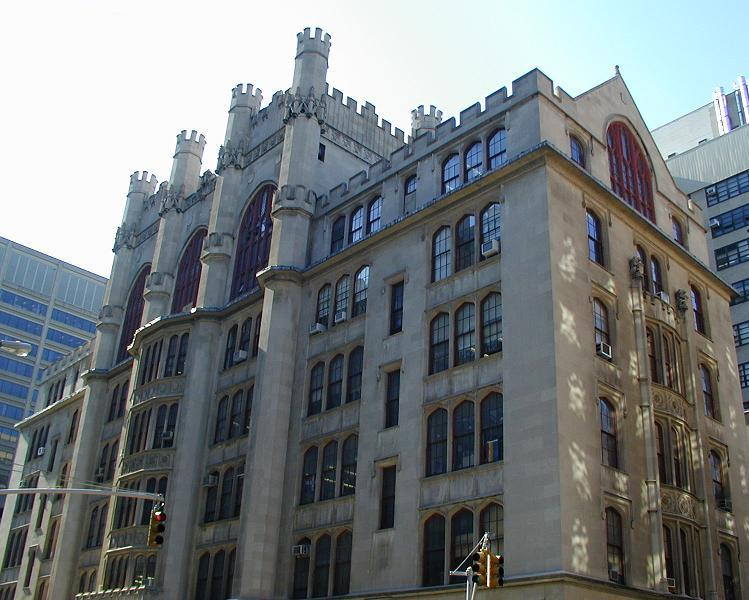
\includegraphics[width=0.6\textwidth]{HunterPhoto.jpg} \\
	(a)\\
	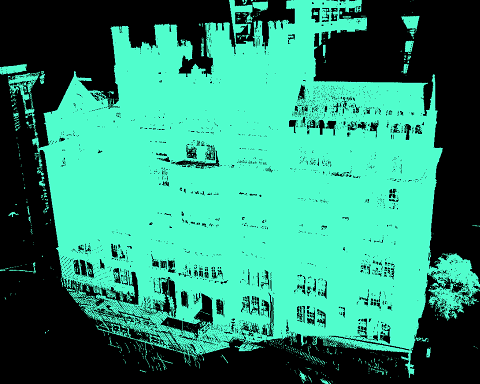
\includegraphics[width=0.6\textwidth]{point_cloud.png} \\
	(b)
\end{tabular}
\end{center}
\caption{
The real point cloud acquisition:
(a) image of building to be modeled;
(b) 3D point cloud of building assembled by registering multiple scans.
}
\label{fig:IR_2_DXF}
\end{figure}

Due to occlusions and limited vantage points, the point cloud collected by the
laser scanner contains artifacts and holes.
In addition, computing directly on 3D data is time-consuming and
computationally complex.
To tackle these issues, we define inner and outer bounding boxes for the
building to clip away unrelated scene objects.
Then, we convert the 3D modeling problem into a set of 2D problems by
projecting the 3D data into a series of 2D cross-sectional contour images.
Noise removal, hole filling, and vectorization are all done in this
2D space.

%%%%% New Chapter %%%%%
%%%%% New Chapter %%%%%
%\newchapt{Data Generation and Acquisition}{chapt_data}{Data Generation and Acquisition}
\newchapt{3D Data Preprocessing}{chapt_data}{3D Data Preprocessing}

The synthetic input data to our system
is unorganized point cloud data (PCD),
namely, no underlying structure information about buildings
is available for modeling.
Furthermore, they were not rectified and
the major facades or planes of the building
were not aligned with the world coordinates.
For the real dataset, although the major axes of the building
have been extracted during the registration stage,
they might be not precise enough for computing major facade planes.
We need to know the major facade planes and their normals in that
they will be used to project PCD to 2D image slices,
which are the starting point for the further computation and inference.
Consequently, as one of the pre-processing stages, the PCD will be transformed
to be aligned with world coordinates along the major planes.

\section{Major Facades Detection}

% 1. Hough space based plane detection.
%
%    After computing the vertical and normals of facades, do the rectification.
% 2. Rectification.
%

Numerous approaches have been proposed on plane and normal detection on PCD.
Based on the techniques used in these approaches,
they can be divided into two different categories.

\begin{enumerate}

\item {\bf Sampling and statistical based:}

The sampling and statistical methods mainly use
the RANdom SAmple Consensus (RANSAC) techniques \cite{RANSAC}
to obtain small set of sampled points for
computing the planes \cite{NE_PVBP,NE_SWK,book_fp}.
RANSAC is widely used in plane detection due to its conceptual simplicity,
generality and reliability on noise.
The RANSAC method computes planes by randomly choosing small sets from
the PCD and constructing corresponding plane parameters.
The resulting candidate plane is tested against all points in the data
to determine how many of the points are well approximated.
After a given number of trials, the plane which approximates the most
points is extracted and the algorithm continues on the remaining data.
However, the major issue of RANSAC is that it would find a wrong plane
if the data has a complex geometry.

In \cite{NE_YF}, the authors tried to overcome the above issue by combining
RANSAC with Minimum Description Length (MDL) which is used to deal with
several competing hypothesis.
They first partitioned the PCD into small rectangle blocks
to ensure that there is no more than three planes in each block.
After this, they applied RANSAC on each block to extract planes.
The MDL is carried out to avoid detecting wrong planes
due to the complex geometry of the 3D data.
Finally, they applied region growing
to merge neighboring planes with certain local range.
The major issue about this method is that it required considerable
computation resource if no further optimizations are applied.

Plane fitting is also widely used for surface extraction from noisy PCD.
Mitra and Nguyen proposed and analyzed a method based on
local least square fitting for estimating the normals
at all sample points of a PCD \cite{NE_MN}.
Given a set of local points $p_i$, $1 \le i \le k$,
they tried to search for a line $a^Tx = c$, with $a^Ta = 1$,
such that the sum of square distance
from the points $p_i$'s to the line is minimized.
Theoretical bound on the maximum angle between the estimated normal
and the true normal of the underlying PCD is computed.
This theoretical study provides a way to find an optimal neighborhood size
to be used in the least square method.

\item { \bf Hough space based:}

This category is a closed-form computation based on Hough space.
Vosselman and Dijkman \cite{NE_VD} proposed 3D Hough transform (HT)
to detect roof planes from PCD acquired from airborne laser altimeter.
Each point $(x, y, z)$ in a laser dataset
defines a plane $z = ax + by + c$ in the 3D parameter space
spanned by the axes of the parameters $a, b$ and $c$,
where $a$ and $b$ are the slopes in $x-$ and $y-$ direction
and $c$ denotes the vertical distance of the plane to the origin.
This representation can work well on detecting near horizontal planes,
as those from airborne laser scanner dataset \cite{NE_GV}.
But it suffers from inferring near vertical planes
due to the potential large value range of the parameters.
Shah improved the representation by defining 3D plane with
its normal direction $\hat{\bf n} = (n_x, n_y, n_z)$ and
its perpendicular distance from the origin $\rho$, which
is able to detect vertical planes efficiently \cite{NE_TRS}.
However, it suffers the discretization problem
when the distance $\rho$ is relative large.
Moreover, since this approach is working on the entire points,
it also requires numerous memory resource when dealing with large-scale PCD.

\end{enumerate}

In order to process large-scale dataset efficiently,
we proposed a plane estimation using
a local plane fitting based normal computation for each 3D point.
By doing local computation, the memory resource requirement is minimized
and the computational requirement is largely reduced.
Although in theory, the accuracy of the normal for each point
is not as precise as those computed globally,
it works well in our case because the majority data points are
those representing the walls/facades of the building.

\subsection{Major Plane Detection}
\label{sec:HS_PD}

The Hough space based plane detection described in Appendix \ref{apdx:HSPD}
can work efficiently if a grid parameterization is available.
However, if such a grid is not available, it will be very inefficient
due to the global quantization of $\rho$ in \Eq{ht_plane}.
To solve this issue, we adopted a local plane fitting method
to compute the normals for each 3D point.
Once we obtain the normals in Euclidean representation,
we can convert it to spherical coordinates representation for quantization.
Hough transform can then be used to identify
the largest $N$ voted normals as the normals of the major planes.
Usually, $N$ is a predefined value by users and represents the number of
facades a building consists of.

We used moving least squares (MLS) for deriving a smooth plane
from a set of neighboring data points in space for normal computation.
A survey of plane detection on point set was done by Cheng {\it et al.} \cite{MLS02}.
Given $n$ points in ${\bf R}^d$, i.e., $\{{\bf x}_i \in {\bf R}^d | i \in [1...n]\}$,
we want to obtain a fitting function $f({\bf x})$ that approximates the given scalar
values $f_i$ at points ${\bf x}_i$.
The idea is to start with a weighted least squares (WLS) formulation
$f'({\bf x})$ for an arbitrary fixed point in ${\bf R}^d$,
and then move this point over the entire parameter domain,
where a WLS fit is evaluated for each point individually.
The fitting function $f({\bf x})$ is obtained from a set of local
approximation functions $f'({\bf x})$:
% general form
\begin{equation}
f({\bf x}) = \underset{f'\in \Pi_{m}^d}{\operatorname{arg\,min}}
\sum_{i=1}^{n}{w_i(\lVert {\bf x} - {\bf x}_i \lVert)\lVert f'({\bf x}_i) - f_i \lVert}
\end{equation}
where $f'$ is taken from $\Pi_{m}^d$, the space of polynomials of total degree
$m$ in $d$ spatial dimensions, and can be written as
\begin{equation}
f'({\bf x}) = {\bf b(x)}^T{\bf c(x)}
\end{equation}
where ${\bf b(x)}$ = $[b_1({\bf x}),..., b_k({\bf x})]^T$ is the polynomial basis vector
and ${\bf c}$ = $[c_1({\bf x}),...,c_k({\bf x})]^T$ is the vector of unknown coefficients,
which we want to minimize.
In general, the number $k$ of elements in ${\bf b(x)}$ is given by
$k = (d+m)!/m!d!$ \cite{MLS01}.
The weighting function $w_i$ is monotonic decreasing as the distance from ${\bf x}$ increases.
There are many options for choosing the weighting function, such as a Gaussian
\begin{equation}
w_i(d) = e^{-d^2/h^2}
\end{equation}
where $h$ is a spacing parameter which can be used to smooth out small features in the data.

% result of general form
Solving the minimization problem by taking partial derivatives with respect to
the unknown coefficients $c_1,...,c_k$, we obtain,
\begin{equation}
{\bf c(x)} = \left[\sum_{i=1}^{n}{w_i(\lVert {\bf x} - {\bf x}_i \lVert)
{\bf b(x}_i{\bf )}{\bf b(x}_i{\bf )}^T}\right]^{-1}
\sum_{i=1}^{n}{w_i(\lVert {\bf x} - {\bf x}_i \lVert){\bf b(x}_i{\bf )}}f_i
\end{equation}

% plane form and result for plane
For our 3D plane fitting, we have $m$ = 1, $d$ = 3 and ${\bf b(x)} = [1, x, y, z]^T$.
The normal is given by the eigenvector of the square matrix
$\sum_{i=1}^{n}{w_i(\lVert {\bf x} - {\bf x}_i \lVert)
{\bf b(x}_i{\bf )}{\bf b(x}_i{\bf )}^T}$
that corresponds to the smallest eigenvalue,
which can be computed using the singular value decomposition (SVD).

% convert N to polar representation and quantization for vote
% in a Hough transform way.

In practice, we use $k$d-tree \cite{NE_KD}
to speed up the query of neighbor points for a given point $P(x_p, y_p, z_p)$
with distance less than a radium $d$.
The construction of a $k$d-tree takes $O(NlogN)$ time,
where $N$ is the number of 3D points.
Querying an axis-parallel range in a balanced $k$d-tree takes $O(N^{1-1/k})$ time,
where $k$ the dimension of the $k$d-tree.
The complexity of MLS is of $O(m)$, where $m$ is the number of neighbor
points for $P$ \cite{MLS03}.
Therefore, the overall major plane detection is of complexity $O(NlogN)$.

%% don't want to show the major plane detection planes.
%% 1. it is not clear. 2. it may need to be shown as a intermediate result.

%% \Fig{ht_plane_hl} shows the major planes highlighted using different colors
%% detected using the proposed Hough space based methods.
%% The walls of the building are detected and shown in red and green.
%% Because the walls parallel to each other have the same or opposite normals,
%% they are detected and highlighted as the same plane, which is appropriate
%% for our application.
%% As mentioned before, the purpose is to project the 3D data into 2D images along
%% the normal of facades.
%%
%% \begin{figure}[htbp]
%% \begin{center}
%% \begin{tabular}{c}
%% 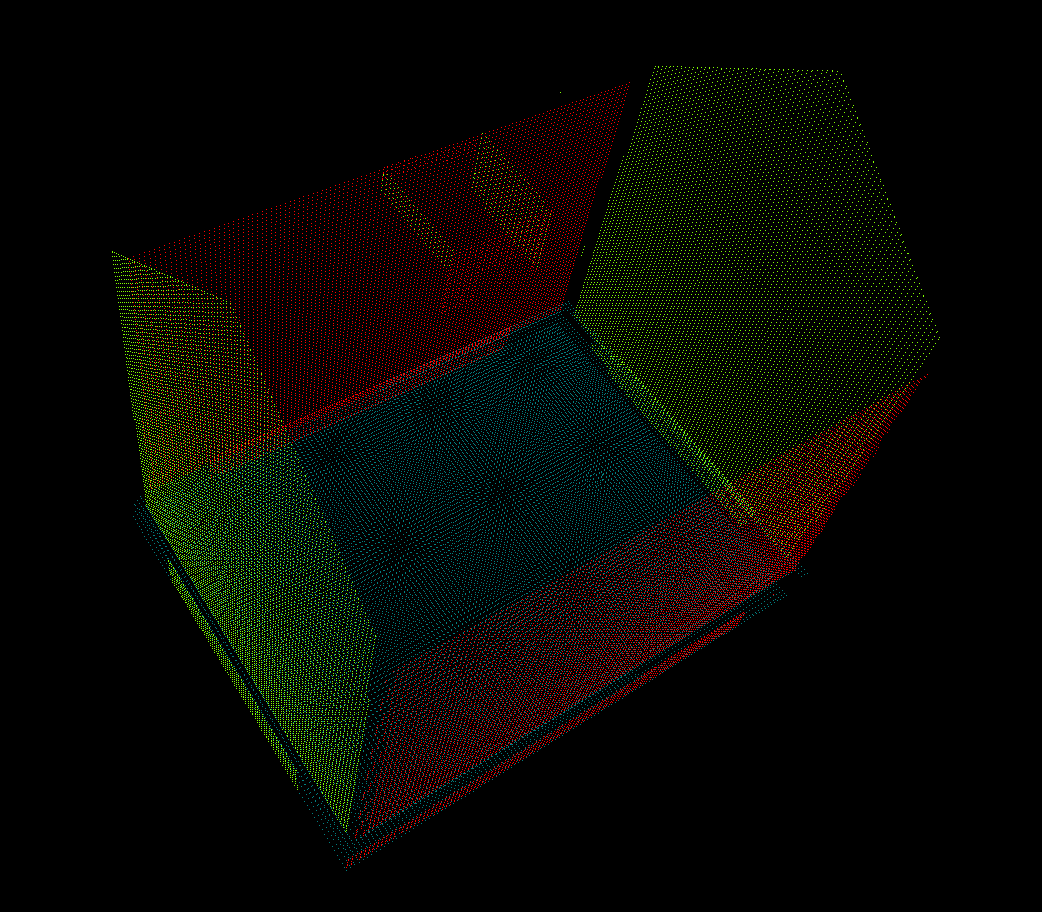
\includegraphics[width=0.6\textwidth]{screenshot_normal.png}
%% \end{tabular}
%% \end{center}
%% \caption{ The detected major planes. }
%% \label{fig:ht_plane_hl}
%% \end{figure}
%%

\subsection{Point Cloud Data Rectification}
\label{sec:rect}

\begin{figure}[htbp]
\begin{center}
\begin{tabular}{c}
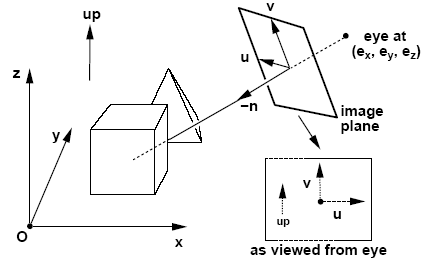
\includegraphics[width=0.5\textwidth]{point_cloud_rect_matrix.png}
\end{tabular}
\end{center}
\caption{ The transformation matrix. }
\label{fig:pc_rect_matrix}
\end{figure}
%% Put the flow of the data rectification.
%% Put the image of rectfied data.
%% \begin{figure}[htbp]
%% \begin{center}
%% \begin{tabular}{c}
%% 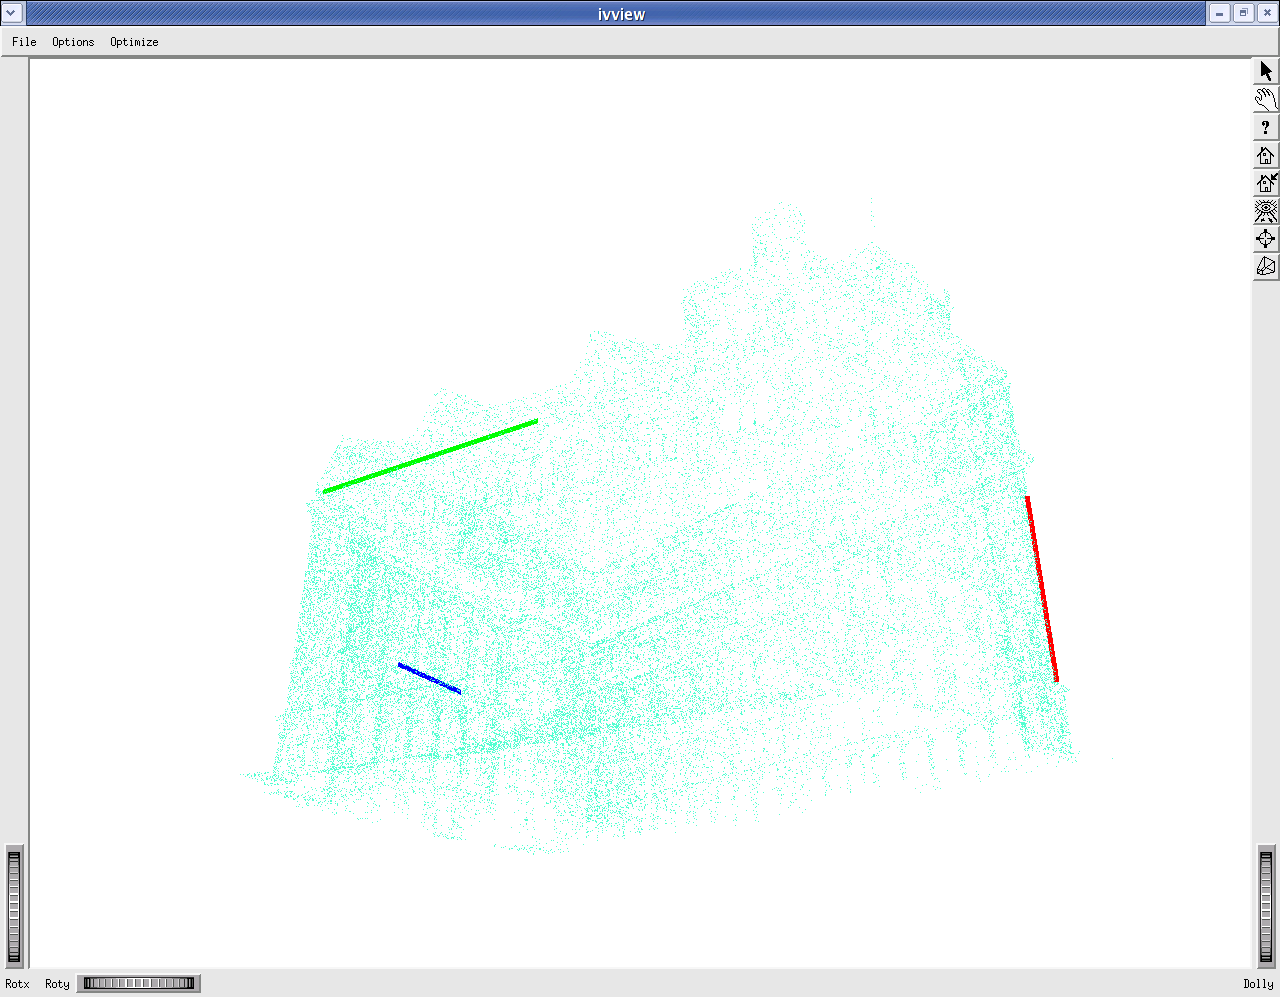
\includegraphics[width=\textwidth]{point_cloud_not_rect.png}
%% \end{tabular}
%% \end{center}
%% \caption{ The registered point cloud without rectification. }
%% \label{fig:pc_orig}
%% \end{figure}

Once the major planes are detected,
we can rectify the original data to generate 2D slices for each major plane.
Assuming $u$, $v$, and $n$ represent the three major axes,
we can rectify the data using the following transformation matrix ${\bf M}$:
\begin{equation*}
\mathbf{M} = \left(
\begin{array}{cccc}
u_x & u_y & u_z & -e_x \\
v_x & v_y & v_z & -e_y \\
n_x & n_y & n_z & -e_z \\
  0 &   0 &   0 &    1
\end{array} \right)
\end{equation*}
This is illustrated in \Fig{pc_rect_matrix}.
$(x, y, z)$ is the world coordinate system.
The rectified coordinate system is represented using $(u, v, n)$.
The vector $[-e_x, -e_y, -e_z]^T$ is the translation
of the view point from the world origin.
In our case, $u$ is the bottom-up vector,
and $n$ is the normal of a major plane
which is perpendicular to $u$.
$v$ is the cross product of $u$ and $n$.
After applying ${\bf M}$,
the original point cloud data is rectified with respect to
each major plane and ready for 2D slice extraction.

%% rectified data
%% \begin{figure}[htbp]
%% \begin{center}
%% \begin{tabular}{c}
%% 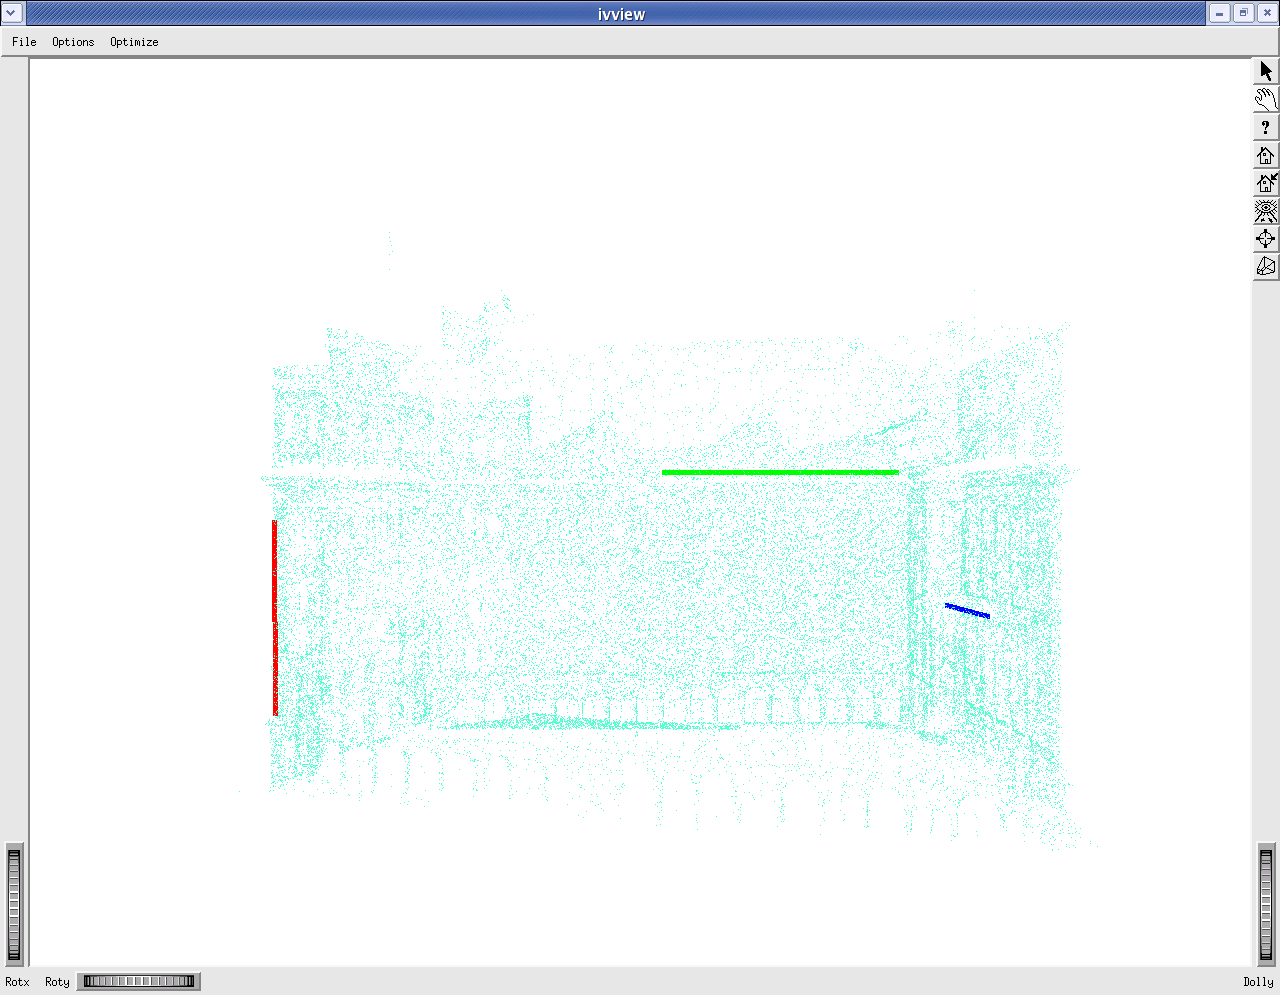
\includegraphics[width=\textwidth]{point_cloud_rectified.png}
%% \end{tabular}
%% \end{center}
%% \caption{ The rectified point cloud of \Fig{pc_orig}. }
%% \label{fig:pc_rect}
%% \end{figure}

%%%%% New Chapter %%%%%
%%%%% New Chapter %%%%%
%\newchapt{2D Slice Extraction and Enhancement}{chapt_pp}{2D Slice Extraction and Enhancement}
\section{2D Slice Extraction and Enhancement}
\label{sec:image_slicing}

We consider the point cloud data as a large array of 3D points to be
sliced into horizontal volumetric slabs.
All 3D points within each slab are projected onto a horizontal projection
plane, or slice, at the base of the slab.
\Fig{slice_slab} shows the 3D point cloud in \Figb{IR_2_DXF}
partitioned into 50 slabs.
The 3D points in each slab are projected onto a projection plane to
form cross-sectional contour slices.
\Fig{slicing} depicts four such slices, associated with the four displayed
projection planes of \Fig{slice_slab}.

\begin{figure} [htbp]
\begin{center}
\begin{tabular}{c}
%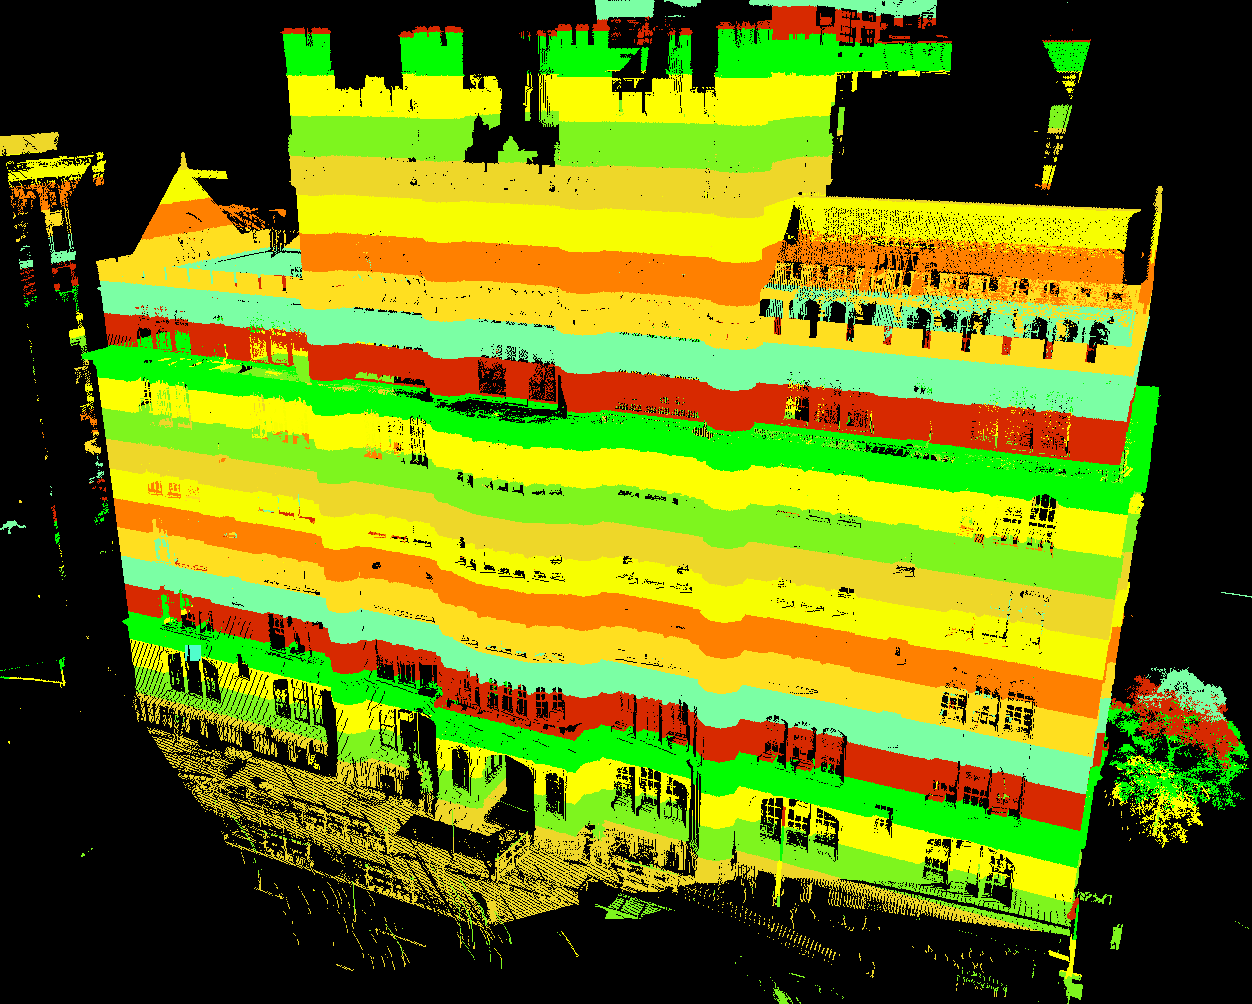
\includegraphics[width=0.6\textwidth]{slab_noplanar.png} \\
%(a) \\
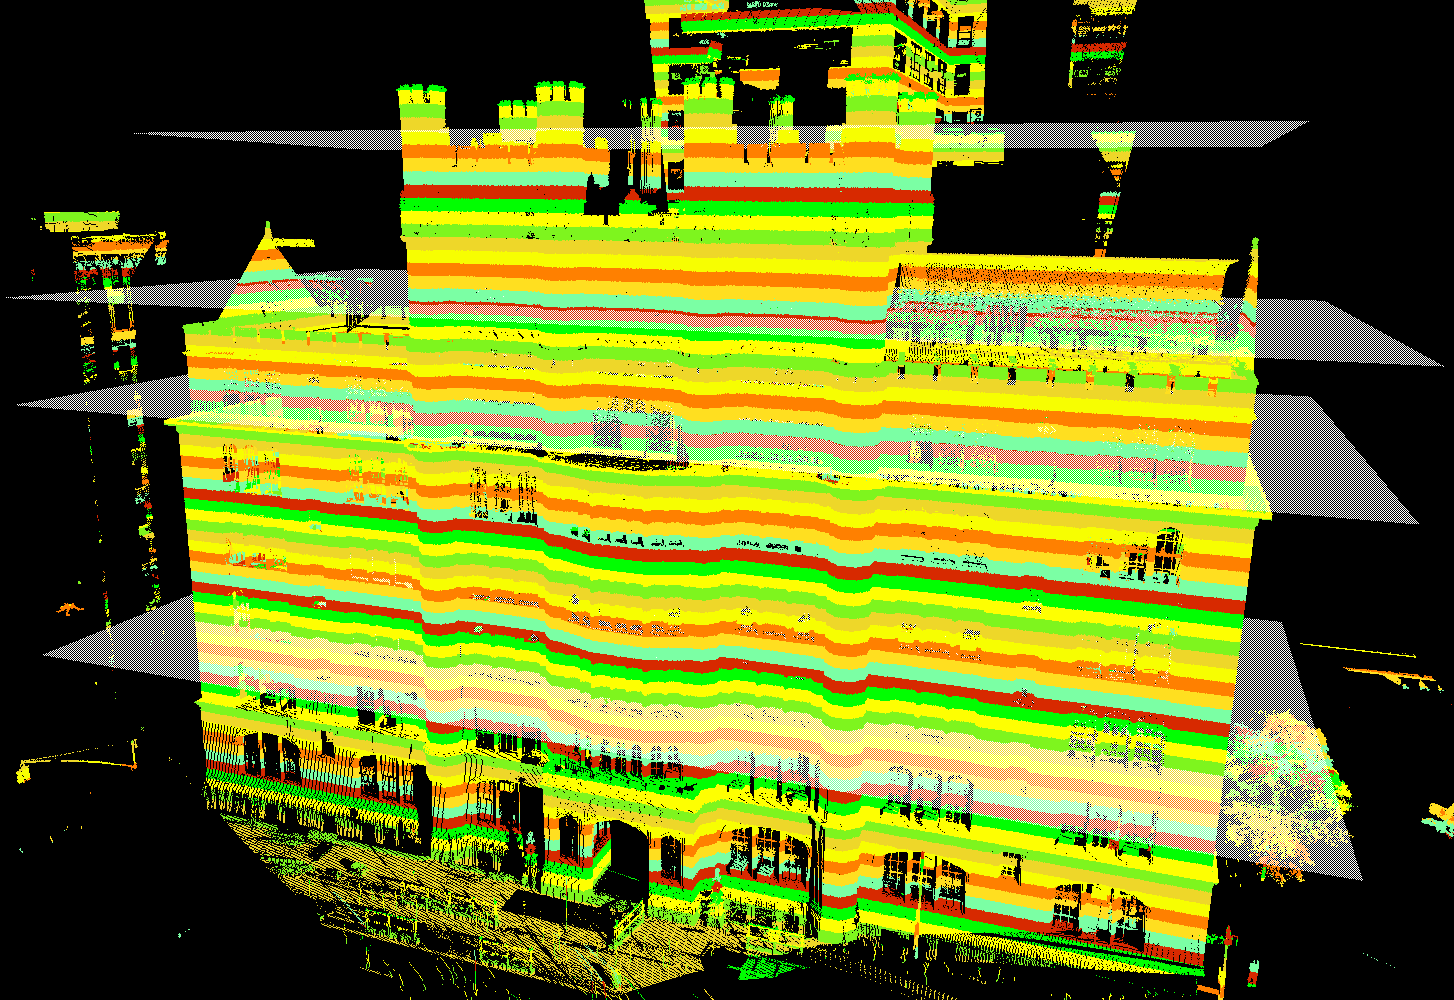
\includegraphics[width=0.6\textwidth]{slab_planar.png}
\end{tabular}
\end{center}
\caption{
%(a) Slabs of the 3D point cloud data are used to determine prominent
%cross-sections upon which extrusion/tapering operations are applied.
The 3D point cloud of \Figb{IR_2_DXF} partitioned into uniform
volumetric slabs.
The 3D points in each slab are projected onto a projection plane to
form cross-sectional slices. Four such planes are shown.}
\label{fig:slice_slab}
\end{figure}

The height of each slab is ${\bf \delta}$.
If ${\bf \delta}$ is held constant, each slice is generated from
equi-spaced slab intervals.
If ${\bf \delta}$ is allowed to vary, then we may
choose to allow for large values in parts of the structure that are similar,
and low values in regions that contain finer detail.
To avoid working on 3D data directly, we choose a relatively small constant value
for ${\bf \delta}$ to generate 2D cross-sectional image slices.

\begin{figure} [htbp]
\begin{center}
\begin{tabular}{cc}
\fbox{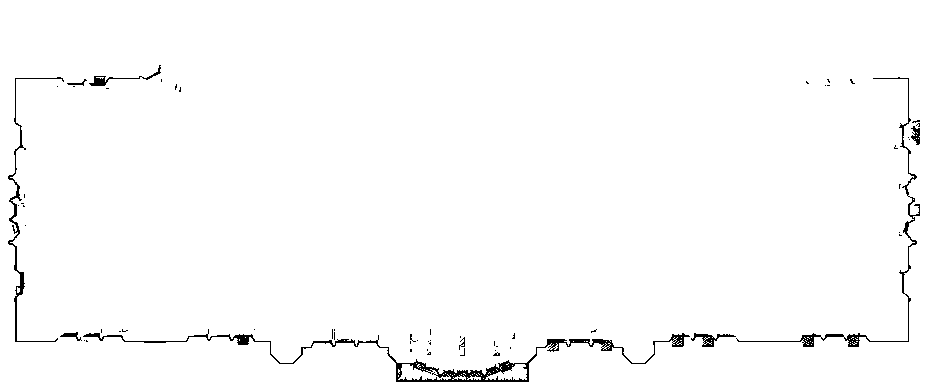
\includegraphics[width=0.45\textwidth]{image_slice_0190.png}} &
\fbox{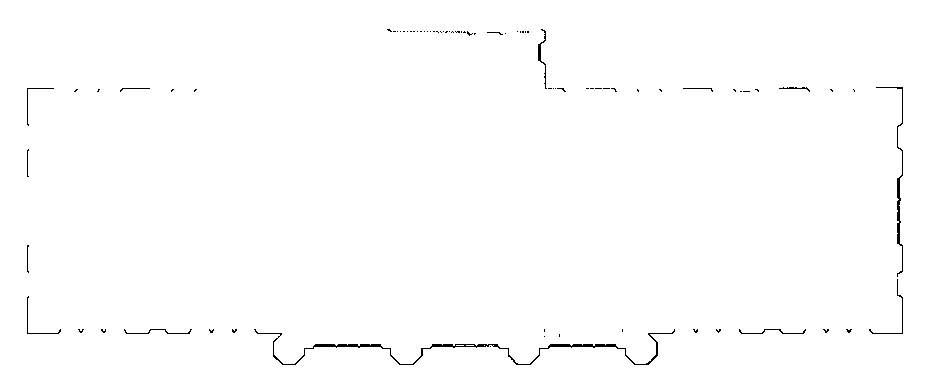
\includegraphics[width=0.45\textwidth]{image_slice_0600.png}} \\
(a) & (b) \\
\fbox{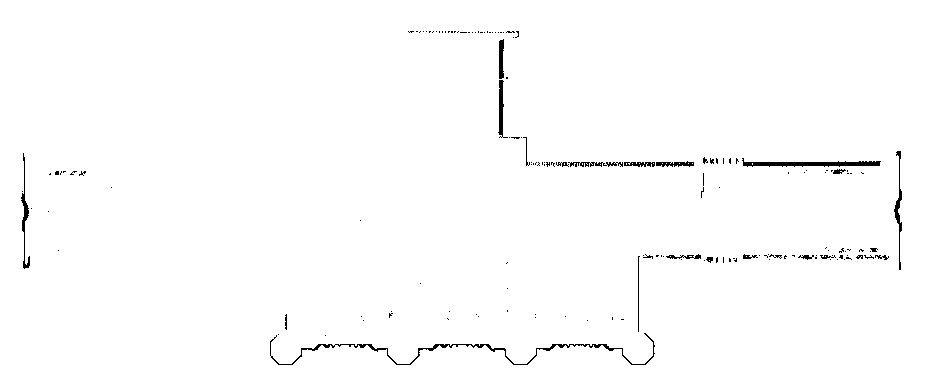
\includegraphics[width=0.45\textwidth]{image_slice_0714.png}} &
\fbox{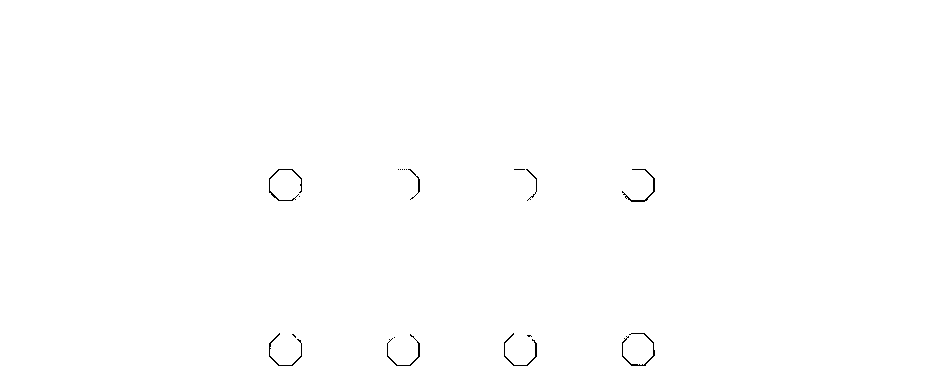
\includegraphics[width=0.45\textwidth]{image_slice_0951.png}} \\
(c) & (d)
\end{tabular}
\end{center}
\caption{The set of slices corresponding to the four projection planes in
\Fig{slice_slab}.}
\label{fig:slicing}
\end{figure}

Without loss of generality,
the $y-$axis is used to represent the bottom-up vertical direction.
Over each slab in height range $[H_{lo}, H_{hi})$,
we project the 3D data ${\bf P}(x,y,z)$, for $H_{lo} \leq y < H_{hi}$,
onto a 2D image slice.
The projection is normalized in the range $[0,W]$, where $W$ is the image width:
\begin{equation}
%[\,x^{2D},\; y^{2D}\,]^T = \omega\cdot[\,x^{3D}_i - X_{min},\; z^{3D}_i - Z_{min}\,]^T
\binom{x^{2D}}{y^{2D}} = \frac{W}{X_{max} - X_{min}} \cdot
\binom{x^{3D}_i - X_{min}}{z^{3D}_i - Z_{min}}
\label{eq:image_slicing}
\end{equation}
%Note that $\omega = W/(X_{max} - X_{min})$, and that
Note that [$X_{min}$, $X_{max}$] and [$Z_{min}$, $Z_{max}$] pairs define the
3D bounding box, which can be obtained through user input and can be used
to clip away noise.

A simple way to implement this 2D slice projection is as follows:
we first compute the total number of slices $N$, i.e.,
$N = (Y_{max} - Y_{min} )/{\bf \delta}$.
For each slab $S_i, \; 1 \le i \le N$,
the height range is $[Y_{min} + {\bf \delta} * (i-1), Y_{min} + {\bf \delta} * i]$.
Once the height range is computed,
we check each 3D data point ${\bf P}(x,y,z)$
whether $y$ is inside this range or not.
If so, one can use \Eq{image_slicing} to
compute the pixel coordinates of the image for ${\bf P}$.
However, the number of 3D point cloud checking would be $N * C$,
where $C$ is the total number of 3D point cloud data.
For a large scale dataset and a reasonable ${\bf \delta}$, this process
is usually slow due to excessive checking and computation.

To improve the performance, we can reduce the number of checking to
be only $C$ by making use of extra memory space.
Basically, for each slab $S_i$, we create a linked-list
which will be used to store all points belong to this slab.
For each 3D data point ${\bf P}(x, y, z)$, we compute its
corresponding slab index $i$ based on $y$ value using the equation,
$i = (y - Y_{min})/{\bf \delta}$.
Then ${\bf P}$ is {\it stored} in the linked-list associated with
the slab with the index $i$.
After going through all the 3D point cloud data once,
the linked-list for each slab is filled with corresponding points.
With the linked-list, it is trivial to generate the sliced image for each slab.
This new implementation largely improved the projection process by reducing
the redundant computation with extra memory space.
\Fig{slicing}(a)-(d) show some examples of the 2D slices, where noise
and incomplete data are observed.


\subsection{Slice Enhancement with Hole Filling}
\label{sec:mdr}

The slices we extract above often have holes (i.e., missing data) due to
occlusion or other visibility issues.
Most urban buildings have symmetry structures
that we can exploit to fill these holes.
Symmetry computation on 3D data is an active research topic
and has potentially numerous applications,
such as those in \cite{Sym_PSGRF,Sym_ZPA,Sym_TW,Sym_MGP}.
However, symmetry computation on 3D data directly is expensive.
Fortunately, we only conduct this computation on 2D image slices.
Furthermore, since the 3D data has been already rectified
and projected onto 2D slices,
we only need to consider 2D translation for symmetry computation.
Let $P(x,y)$ be a point on the original image $I$.
Let $P'(x',y')$ be the reflected point of $P$ with respect to a symmetry line $L$.
The symmetry computation equation for $L$ is as follows:
\begin{equation}
L = \underset{x,y}{\operatorname{arg\,min}}\sum{d_{x,y}(P', I)}
\end{equation}
where the $d_{x,y}(P',I)$ is the distance between the self-reflected point
$P'$ and its nearest data point in image $I$.
The reflected point $P'$ of the original point $P$ is computed with
respect to a line along either the $x-$axis or $y-$axis.
Therefore, the symmetry line $L$ is obtained as the line with minimum
summation error over the reflected data points.
\Figa{sym} depicts the original input sliced image with holes.
The result after hole filling using symmetry computation is shown in \Figb{sym}.

\begin{figure}[htbp]
\begin{center}
\begin{tabular}{c}
\fbox{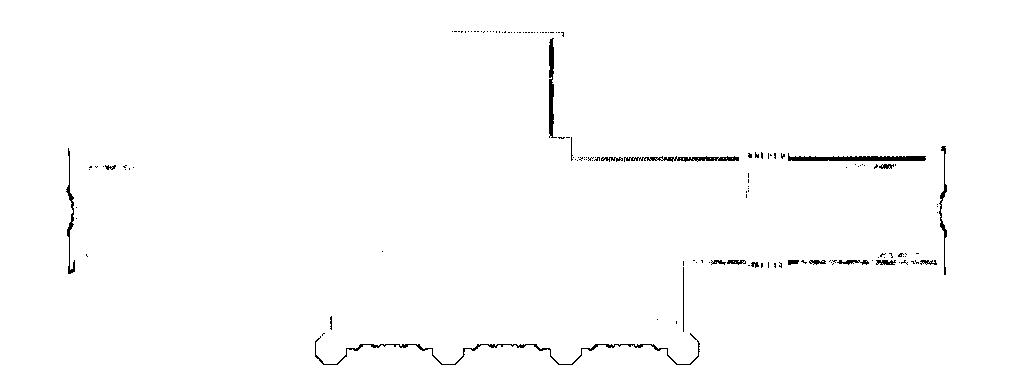
\includegraphics[width=0.6\textwidth]{image_slice_0705_0711.png}} \\
(a) \\
\fbox{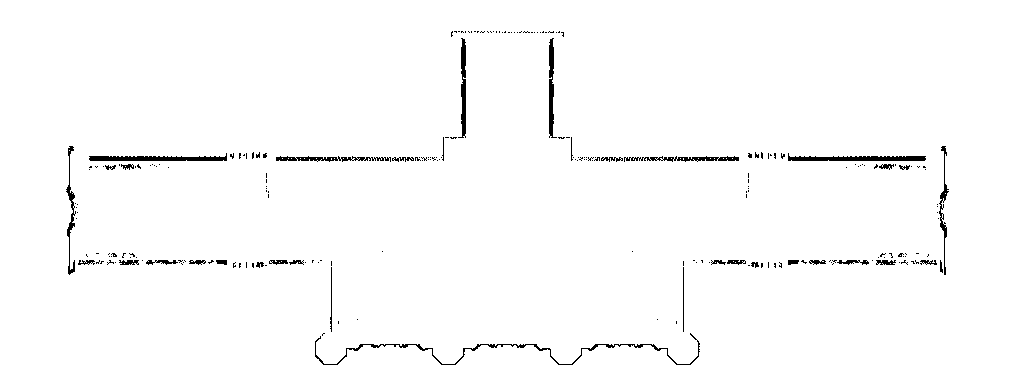
\includegraphics[width=0.6\textwidth]{image_slice_0705_0711_recoverd.png}} \\
(b)
\end{tabular}
\end{center}
\caption{ Symmetry-based hole filling: (a) original 2D slice image;
(b) enhanced image after hole filling.}
\label{fig:sym}
\end{figure}

%%%%% New Chapter %%%%%
%%%%% New Chapter %%%%%
%\newchapt{Dataset Segmentation}{chapt_segment}{Model Segmentation}
\section{Dataset Segmentation}
\label{sec:mseg}

Modeling a building PCD as a whole structure simultaneously
is complicated due to the natural complexity of buildings.
To simplify this problem,
We utilize the divide and conquer strategy
to segment the whole PCD of a building into simpler ones.
Following this, we reconstruct each segmented
part based on extrusion or tapering operations.
Once each segment is processed and modeled,
the whole PCD can be combined and merged into the final model.

3D point cloud data segmentation has been an active research topic for years,
and Hoover {\it et al.} compared a variety of methods
for finding planar segments in range images \cite{MS_HOO}.
Essentially, segmentation is the process of labeling each data point
so that the points belonging to the same structure are grouped together.
Based on the techniques used for segmentation,
the proposed algorithms can be roughly categorized into two groups.

\begin{enumerate}

\item {\bf Edge based method:}

Edge based methods first apply edge detector to
extract the boundary edges of different regions.
The edges are detected based on the local surface properties,
such as surface normals, gradients, principal curvatures,
or higher order derivatives.
These edges include jump edges, crease edges and smooth edges \cite{MS_JBU}.
Jump edges are defined as discontinuities in depth values,
which are observed when an object is occluded by another one.
Crease edges are characterized by discontinuities in surface normals,
which are formed where two regions meet.
Smooth edges are those with continuous surface normals but
discontinuous curvatures.
The second stage of these methods is to link these detected edges
to form closed regions for segmentation \cite{MS_SV,MS_KS}.

The main weakness of these methods is that
they cannot guarantee closed boundaries
for the complicated situations where some edge points
may not be correctly detected.
To tackle this issue, edge detection based on
scan line approximation are proposed as in\cite{MS_SD,MS_KMK,MS_JB}.
Scan-line based methods first project the range data into
binary edge map along a given direction or scan line.
For example, a scan line on 3D plane produces a 3D straight line.
After projection, scan line segments are merged together
based on some similarity measure in a region-growing fashion.
Finally, some edge grouping techniques, such as
minimum spanning tree, are applied to obtain closed contours
for segmentation.
The scan line method is mainly designed to extract planar surfaces.

Heath {\it et al.} compared some well-known edge detectors,
such as Canny, Nalwa-Binford, Sarkar-Boyer and Sobel \cite{MS_HSSB}.
There are several criteria they used for comparison:
For each edge detector,
is it possible to choose a single set of optimal parameters
for all the images without significantly affecting the performance?
Does an edge detector produce edges of the same quality for all images
or does the edge quality vary with input images?
They found that the optimal parameter settings of an edge detector
are strongly dependent on the input images,
and that the relative performance of the edge detectors varied
statistically significantly across the input images.
This indicates the performance of the dataset segmentation
might be affected by the parameter settings of its edge detector
and there is no optimal detector that can be used for any input data.


\item {\bf Region based method:}

The majority work on range image segmentation relied on
region-based techniques \cite{MS_XW,MS_RHV,MS_PV}.
These methods are relatively less sensitive to the noise in the data,
and usually perform better when compared to edge-detection methods.
First, seed regions which can be planar or non-planar
surface patches are computed.
Least squares adjustment and Hough transform are robust methods
to detect planar seeds.
The seed regions are then gradually growing to larger region
by grouping points around them based on the given similarity measure,
such as slope, curvature or surface normal.

Region based approaches are essentially focusing on local features
and their consistencies in the data.
For example, Hernandez {\it et al.} extracted features from connected components
based on Top-Hat of hole filling algorithm of range images \cite{MS_HMP}.
Although these techniques bring acceptable results,
they suffered from some common issues,
such as the selection of the initial seed regions
and the determination of the number of clusters.
Some global features based on graph techniques are proposed to improve
segmentation results.
Graph cut in \cite{MS_SM,MS_BK} and minimum spanning tree in \cite{MS_HK}
are widely used graph based algorithms.
The observation is that data points in the same segment
are much more closely connected to each other
compared with those points in other segments.
The segmentation is achieved by graph partitioning algorithms to
find the optimized cuts that minimize the similarity between segments
while maximizing the similarity within segments at the same time.
Segmentation can be performed as recursive partitioning
or direct multi-way partitioning as in \cite{MS_SZ}.

Computational cost for region based methods is usually much higher
compared with edge based methods.
It is not really an issue when small range images are considered.
However, this high-demanding of the computational resources prevent
them from being used on large-scale point cloud datasets.

\end{enumerate}


%% (OPTION) We proposed a multi-resolution segmentation approach,
%% that is separator based and keyslice based segmentation.
%% The idea is to first decompose the whole building using separator slices detected from
%% all major facades. This segmentation step is relative safe and precise in a sense that
%% the separators or salient planar feature generally separate parts from each other.
%% The segmentation consists of two steps;
%% the first one is separate the data based on separators detected
%% in slices from all major directions. We shall obtain split data after the first step.
%% The second step is to further segment these split data if necessary.

These proposed approaches on dataset segmentation are either not applicable to
the building PCDs or computational expensive.
We proposed an efficient segmentation approach for building PCD
based on the observation that different parts of a building
are usually separated by walls, ledgers etc.
These {\it ``separators''} provide clues for dataset segmentation.
When projected onto 2D images, these separators have a common characteristic,
that is a relative large {\it ``dark''} region
representing a salient feature in binary images.
For example, the roof and the body are divided by a ledger as shown in \Figc{MS_Fig1}.
\Figb{MS_Fig1} and \Figd{MS_Fig1} shows different parts of the roof are separated by walls.


\begin{figure}[htbp]
  \centering
  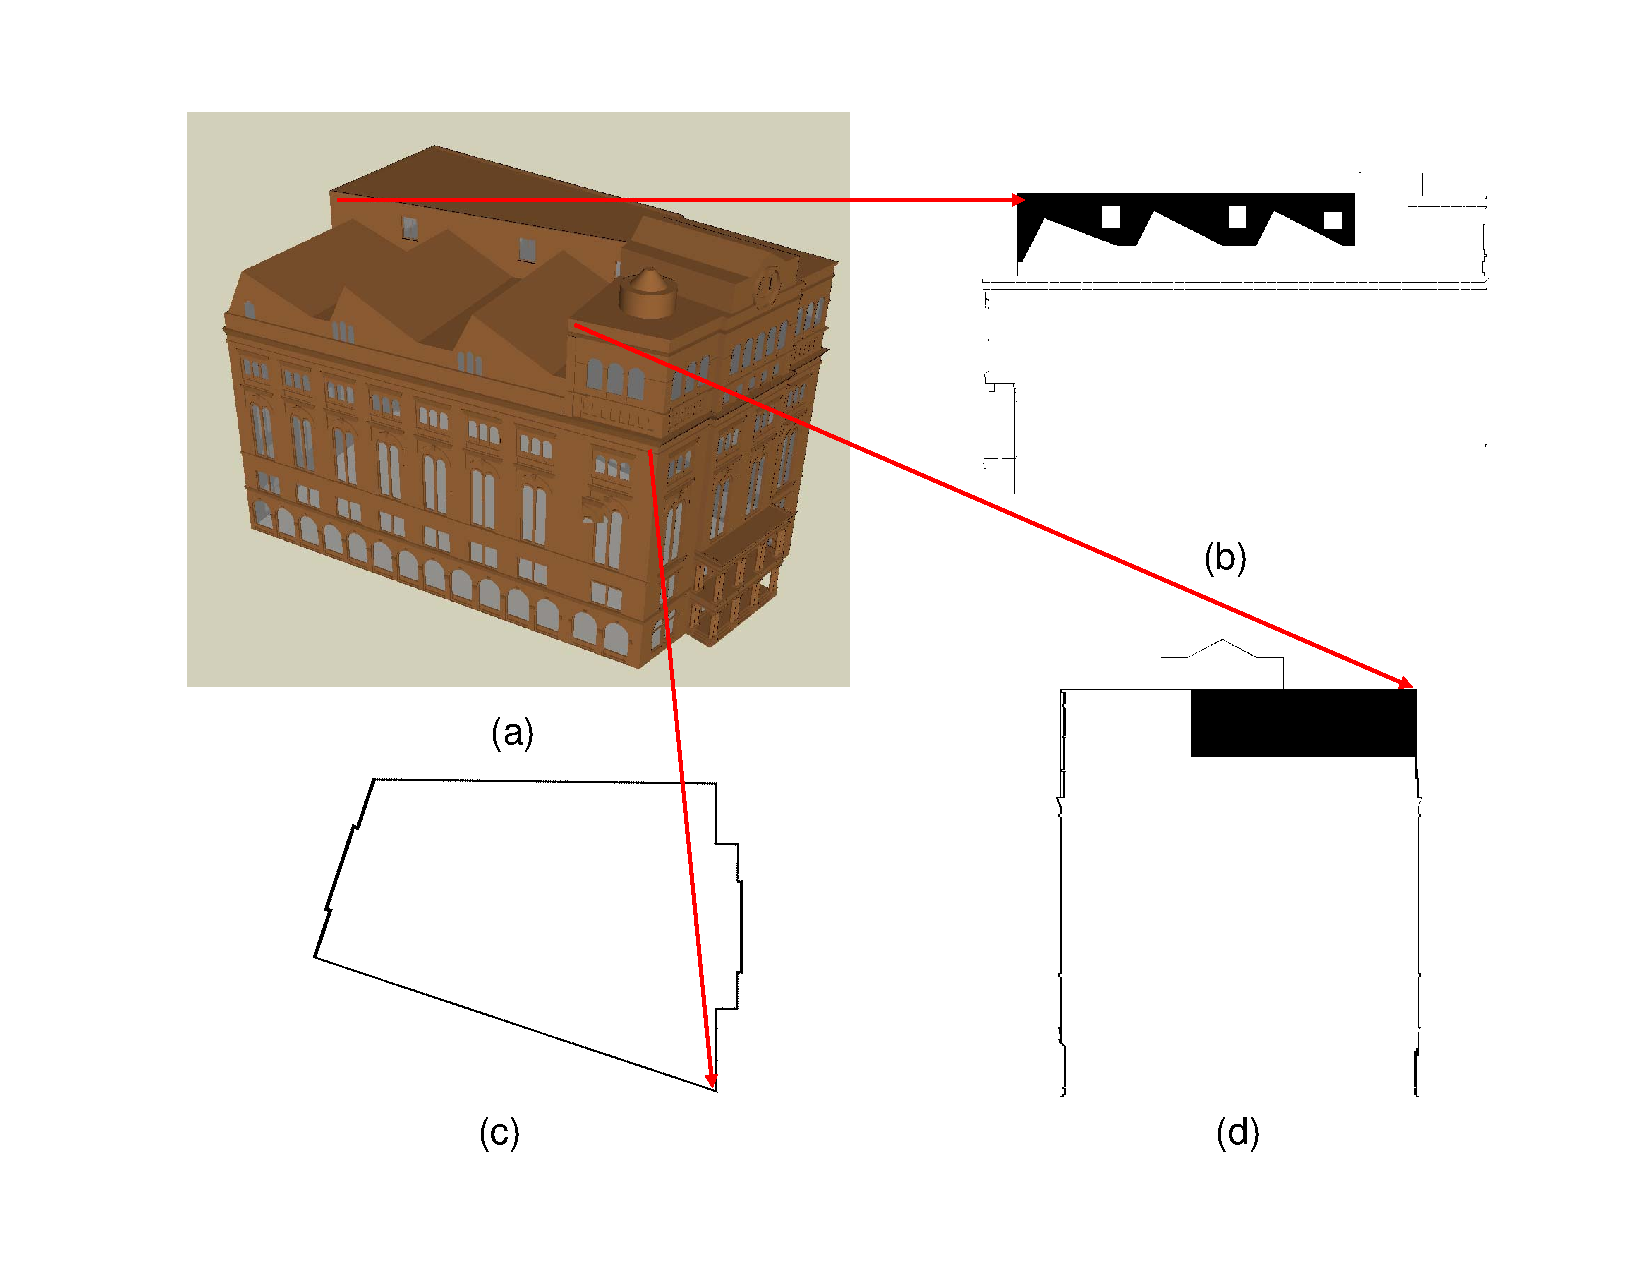
\includegraphics
      [width=\textwidth]
      {model_separate.pdf}
      \caption{The dataset segmentation:
      (a) the original cooper union model;
      (b) the projected wall image from one face;
      (c) the projected ledger image;
      (d) the projected wall image from another face.}
      \label{fig:MS_Fig1}
\end{figure}

The dataset segmentation is carried out as follows.
First, for a given point cloud dataset,
we compute separators from all major directions obtained earlier,
including bottom-up direction and directions perpendicular to major planes.
The next step is to split the original 3D dataset into segments
based on the computed separators together with direction information.
We will elaborate these steps in the following sections.

\subsection{Separator Detection}
\label{sec:sd}

We used a kernel based connected components (CC) method for computation.
For each identified slice image $I_i$, the separator detector
checks each data point $P_i$ using a $5$x$5$ kernel $K$ centered at $P_i$.
Let $S_p$ be a set of points that have been visited by the separator detector.
$S_p$ is initialized to be empty.
The point $P_i$ is checked against $S_p$ to
determine whether it has been visited previously.
If not, $P_i$ is added into $S_p$ and
the data points $N=\{P_j | P_j \neq P_i, P_j \in K\}$
covered by the kernel $K$ are recorded.
If there are enough data points found in the neighbor,
say $|N| > 12$, namely half of the kernel $K$,
$P_i$ is considered as qualified point for the connected component
and is added to $C$.
The same computation is applied to all new recorded data point in $N$,
and qualified points are added into $C$.
When there is no more new data point needs to be checked, the detector stops
and a new connected component, $C$, is detected.

The next step is to compute the rectangle boundary of $C$,
$\{x_{min}$, $x_{max}$, $y_{min}$, $y_{max}\}$.
To check whether $C$ represents a qualified separator,
the following test is conducted,
\begin{equation*}
\left\{
\begin{array}{lr}
| x_{max} - x_{min} | > T_{size} \\
| y_{max} - y_{min} | > T_{size}
\end{array} \right.
\end{equation*}
where $T_{size}$ is a threshold representing the minimum size of the separator,
usually a value of $16$ is good enough to rule out all non-separators.
The above testing implies that a real separator CC
should contain a big chunk of data
and its width and height should be at least $T_{size}$.
If a connected component $C$ satisfies the above conditions,
the slice index $i$ together with the bounding information
$x_{min}, x_{max}, y_{min}, y_{max}$,
are logged down for further process.

\begin{figure}[htbp]
\begin{center}
\begin{tabular}{cc}
\fbox{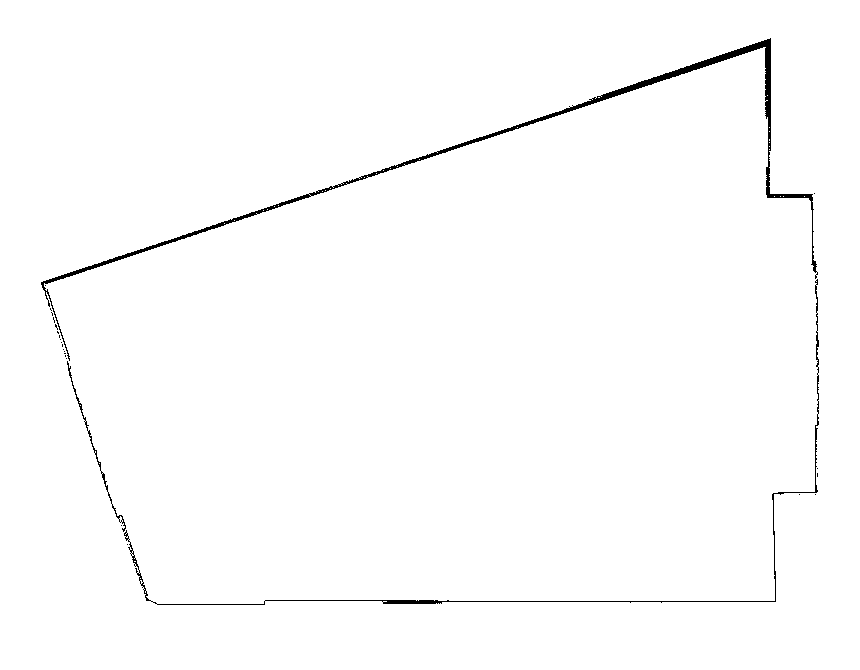
\includegraphics[width=0.45\textwidth]{segment_slice_0091.png}} &
\fbox{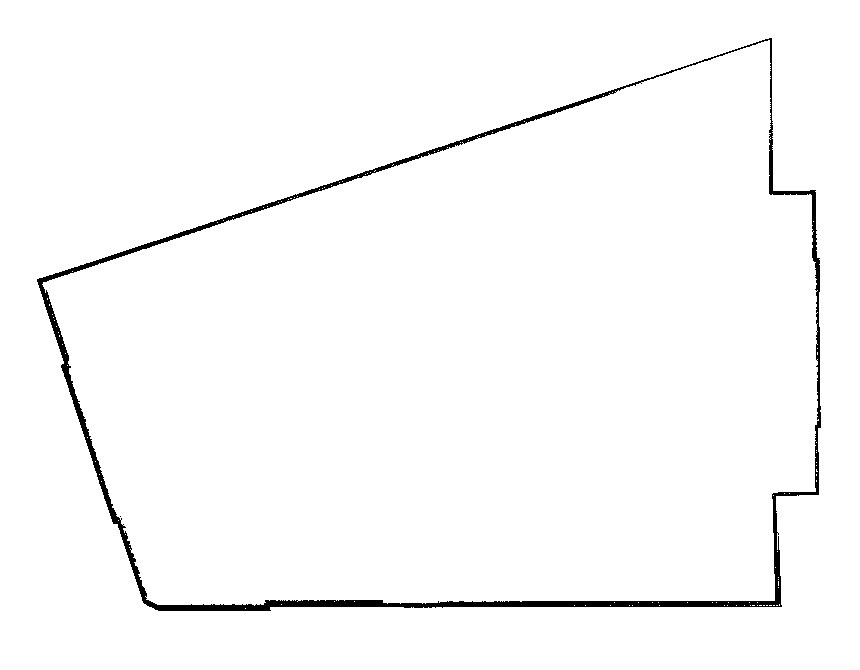
\includegraphics[width=0.45\textwidth]{segment_slice_0092.png}} \\
(a) & (b) \\
\\
\fbox{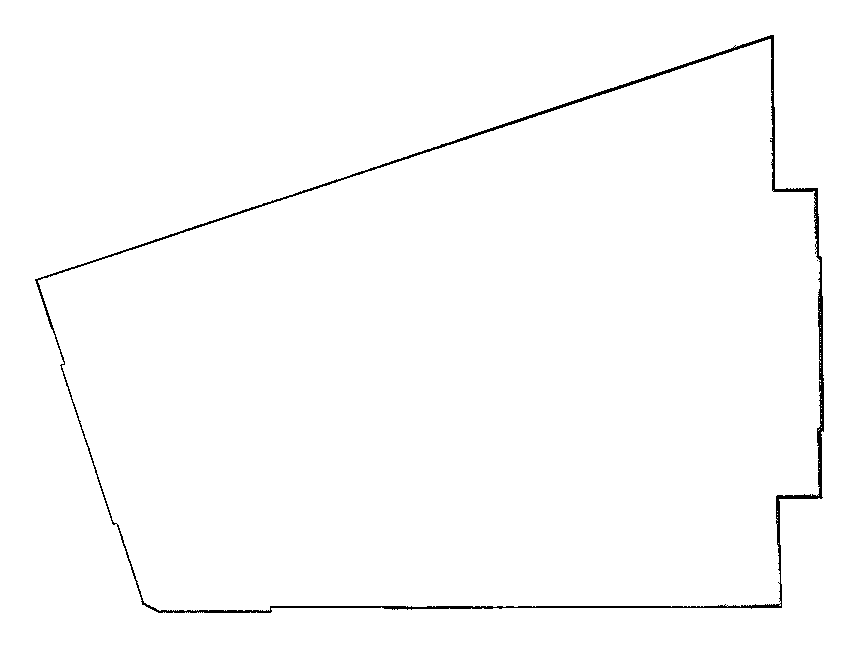
\includegraphics[width=0.45\textwidth]{segment_slice_0093.png}} &
\fbox{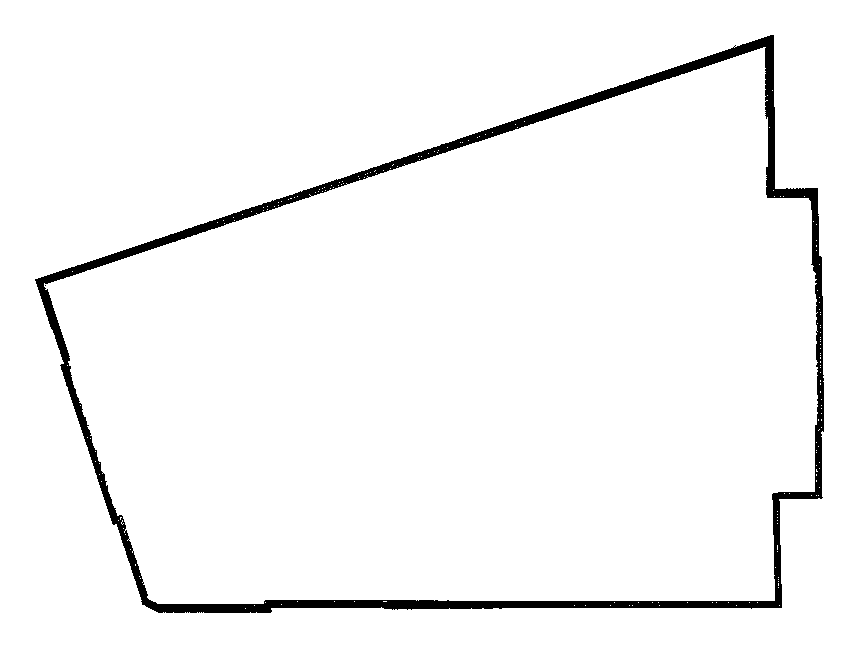
\includegraphics[width=0.45\textwidth]{segment_merged_slice_all.png}} \\
(c) & (d) \\
\end{tabular}
\end{center}
\caption{The adjacent slices with separators detected:
(a) the first slice;
(b) the second consecutive slice;
(c) the third consecutive slice;
(d) the merged slice from (a) to (c).
}
\label{fig:segment_merged}
\end{figure}

For real dataset, separators might be detected in adjacent or
neighboring sliced images as shown in \Fig{segment_merged} (a) - (c).
This is usually caused by imperfect major plane detection
or point cloud data registration introduced in earlier stages.
To cope with this case automatically,
we integrate all the neighboring sliced images
with separators detected into a new image $I$ as shown in \Figd{segment_merged}.
And the same separator detection algorithm is applied on $I$
to obtain the bounding information.
The index for this integrated image is set to be the mean
of the indices of those neighboring images.
After this automatic computation, we present the results to users
and allow them to adjust the results manually.
Essentially, users can adjust the index of the integrated image,
which could avoid any potential errors for segmentation.

\subsection{Segmentation Based on Separators}

%%% TWO PARTS:
%%% 1. segmentation on 2D slices.
%%% 2. demonstration on 3D PCD.

%%% show (c) and (d) for 3D PCD segmentation.
%%% show (a), (b) and their superimpose images as 2D slice segmentation.
%%% for 2D sliced image segementation, show a superimposed image and its
%%% segmented region with each region shown as a small image in PPT.

Once we have computed the separators based on the 2D sliced images
extracted from all major directions,
we can divide the original complex building structures into
smaller and simpler modules for modeling.
Based on the type of the input data we are about to segment,
two approaches could be adopted for this partitioning process.
First, the segmentation can be carried out on
the original 3D point cloud dataset.
That is, a series of smaller 3D point cloud datasets will be
generated for each segment.
However, for this approach, we have to transform each
smaller segment and generate the projected 2D images
for each major facades.
This would impose redundant projection
and the noise removal and hole filling would have to be applied again.
Alternatively, we can apply the segmentation directly on
the 2D sliced images generated previously,
and therefore avoid those redundant transformation
and projection computation required for the first approach.

\begin{figure} [htbp]
\begin{center}
\begin{tabular}{cc}
\fbox{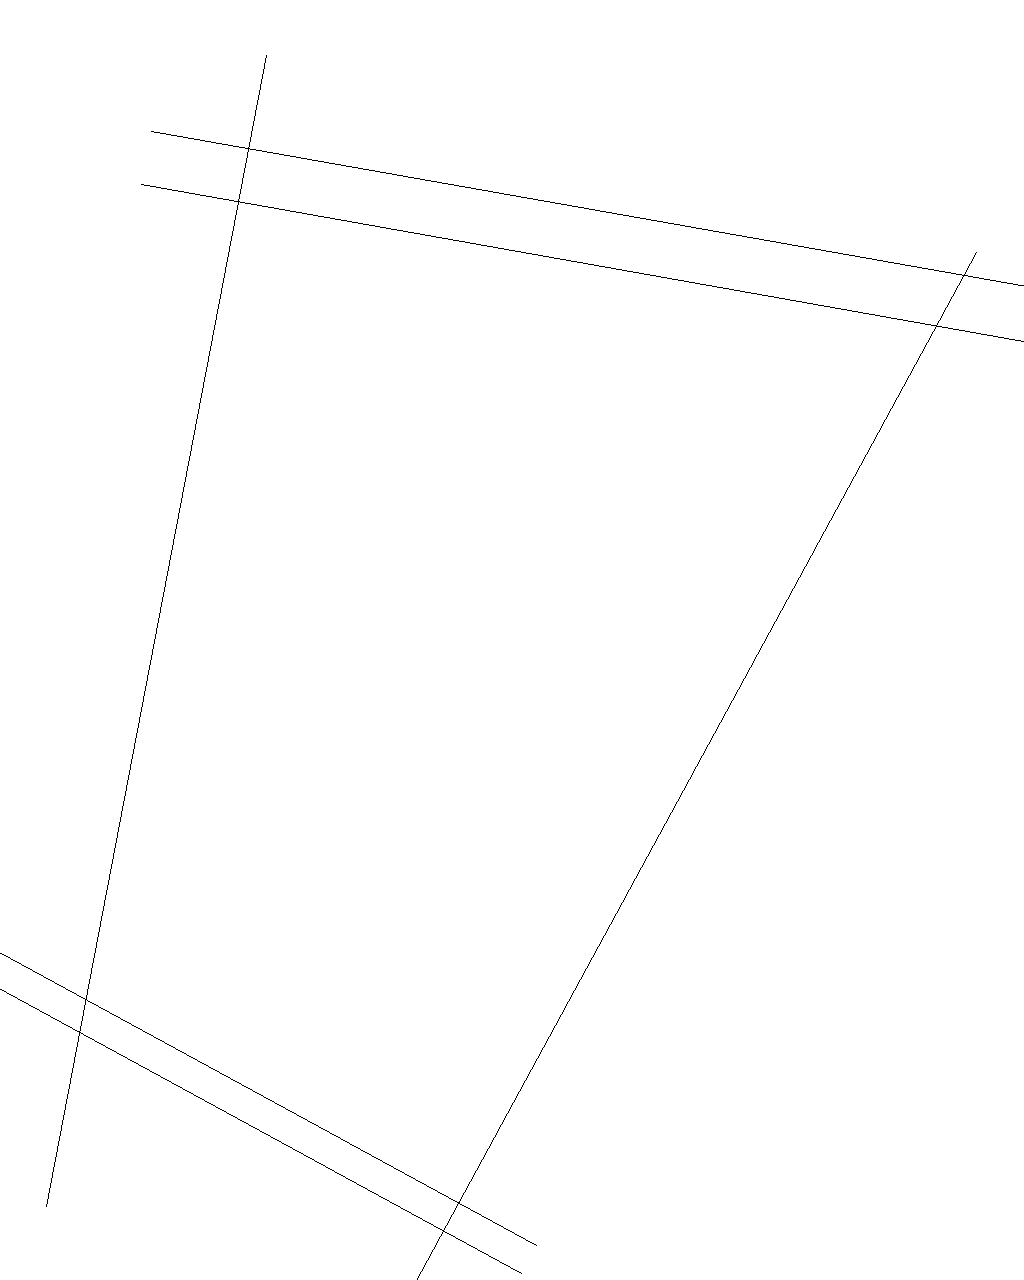
\includegraphics[width=0.4\textwidth]{segment_body_result.png}} &
\fbox{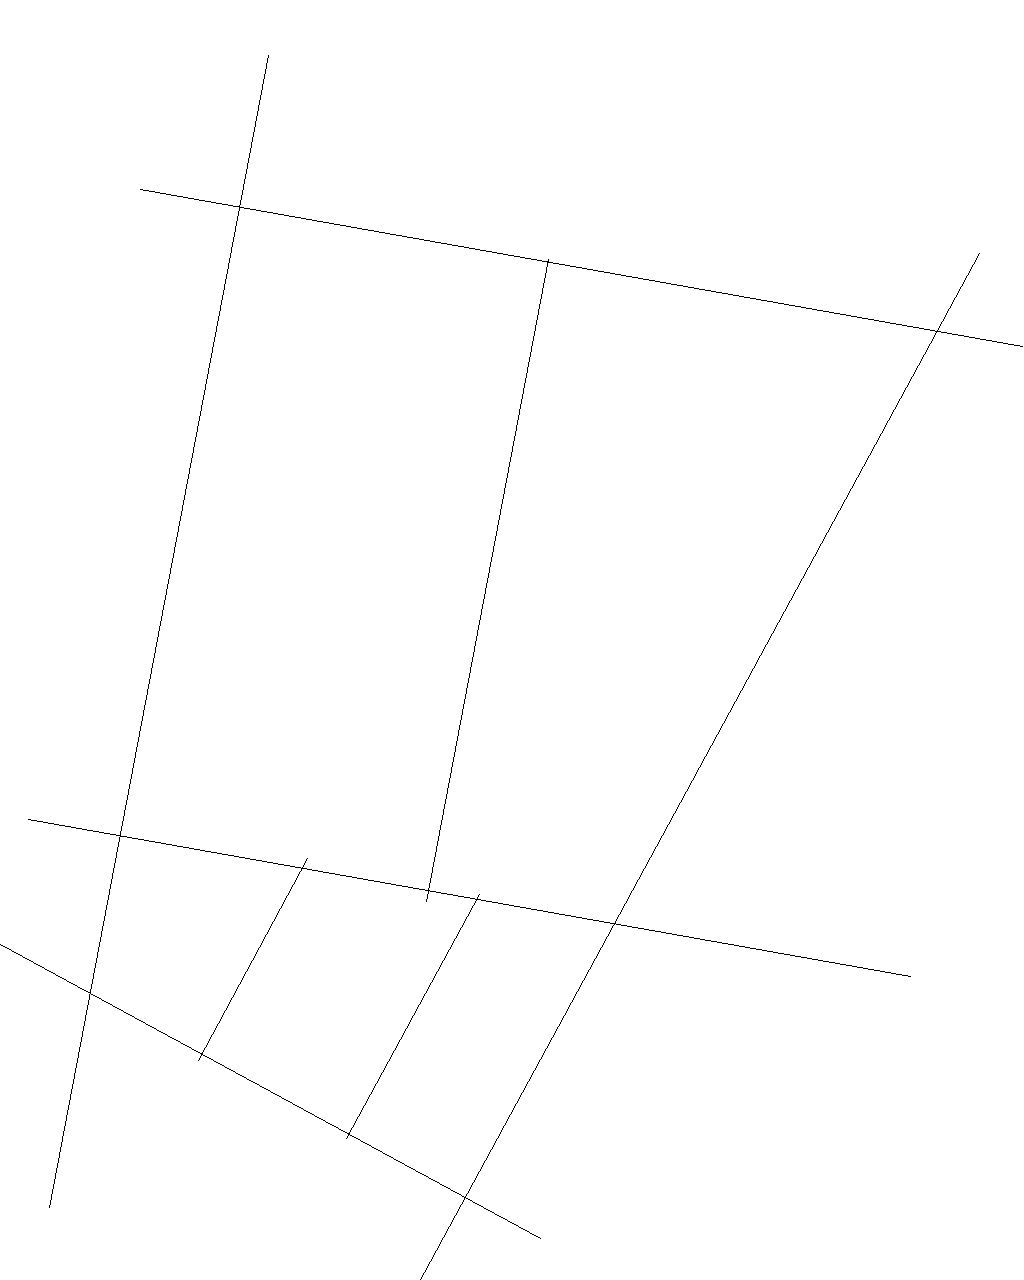
\includegraphics[width=0.4\textwidth]{segment_roof_result.png}} \\
(a) & (b) \\
\fbox{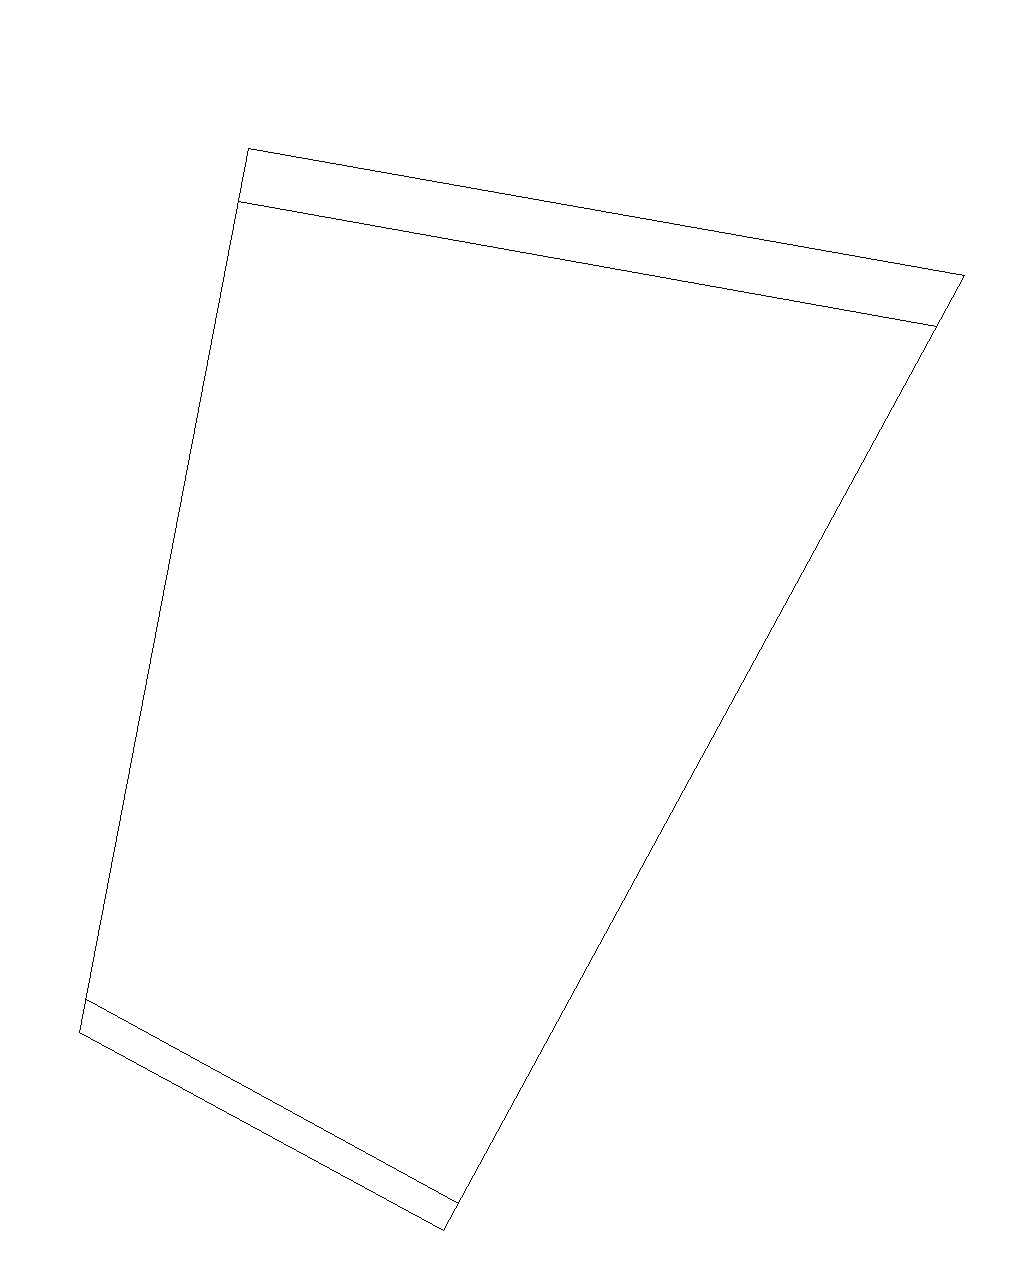
\includegraphics[width=0.4\textwidth]{segment_body_result_region.png}} &
\fbox{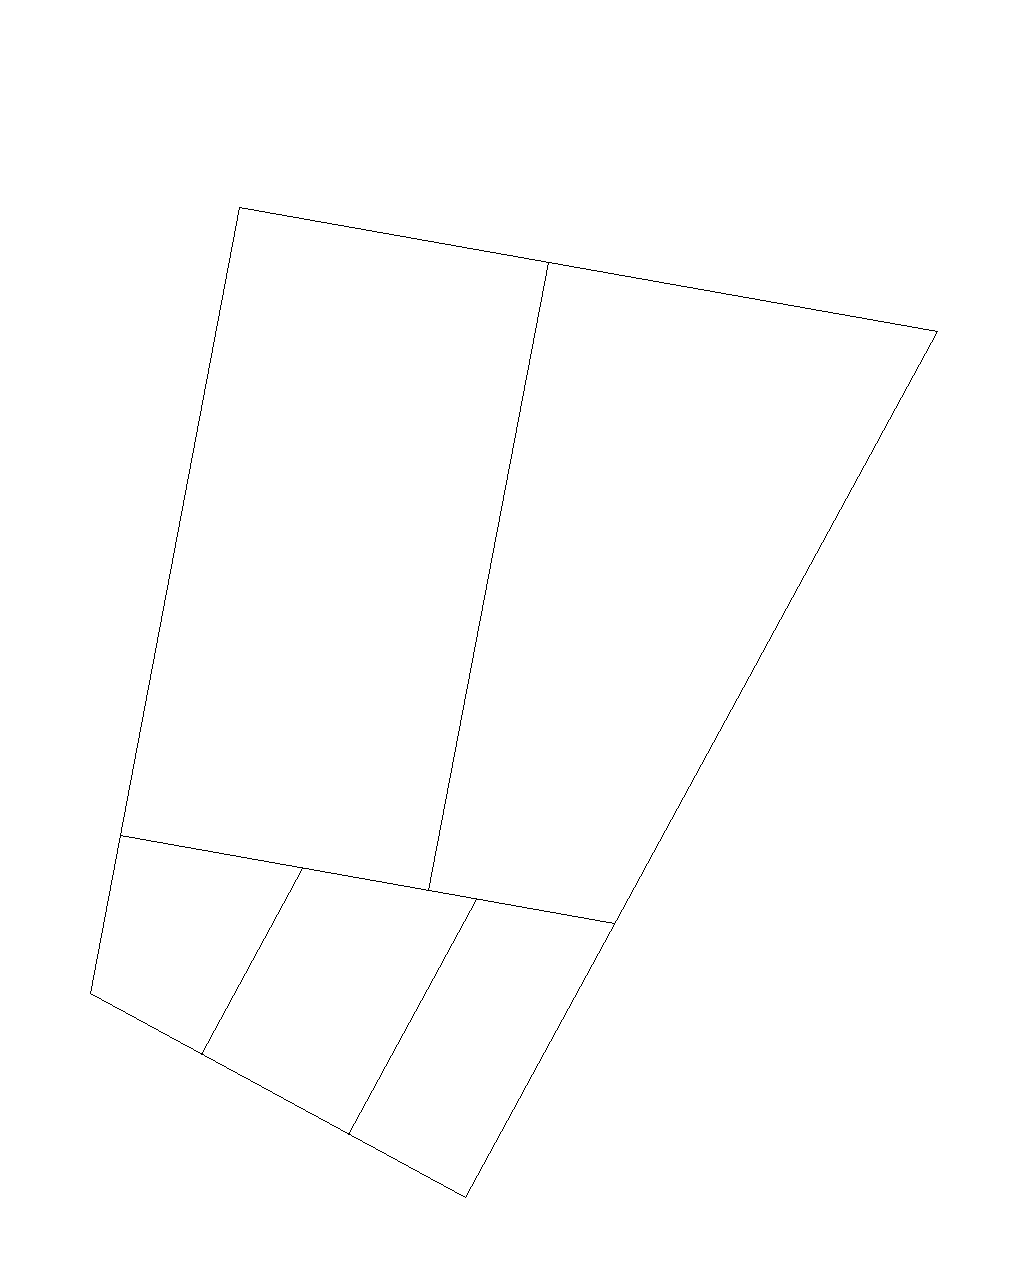
\includegraphics[width=0.4\textwidth]{segment_roof_result_region.png}} \\
(c) & (d)
\end{tabular}
\end{center}
\caption{ Segmentation region computation:
      (a) the transformed image with line segment of the separators for body;
      (b) the transformed image with line segment of the separators for roof;
      (c) the processed segment image regions for body;
      (d) the processed segment image regions for roof. }
\label{fig:DS_Fig1}
\end{figure}

\begin{figure} [htbp]
\begin{center}
\begin{tabular}{cc}
\fbox{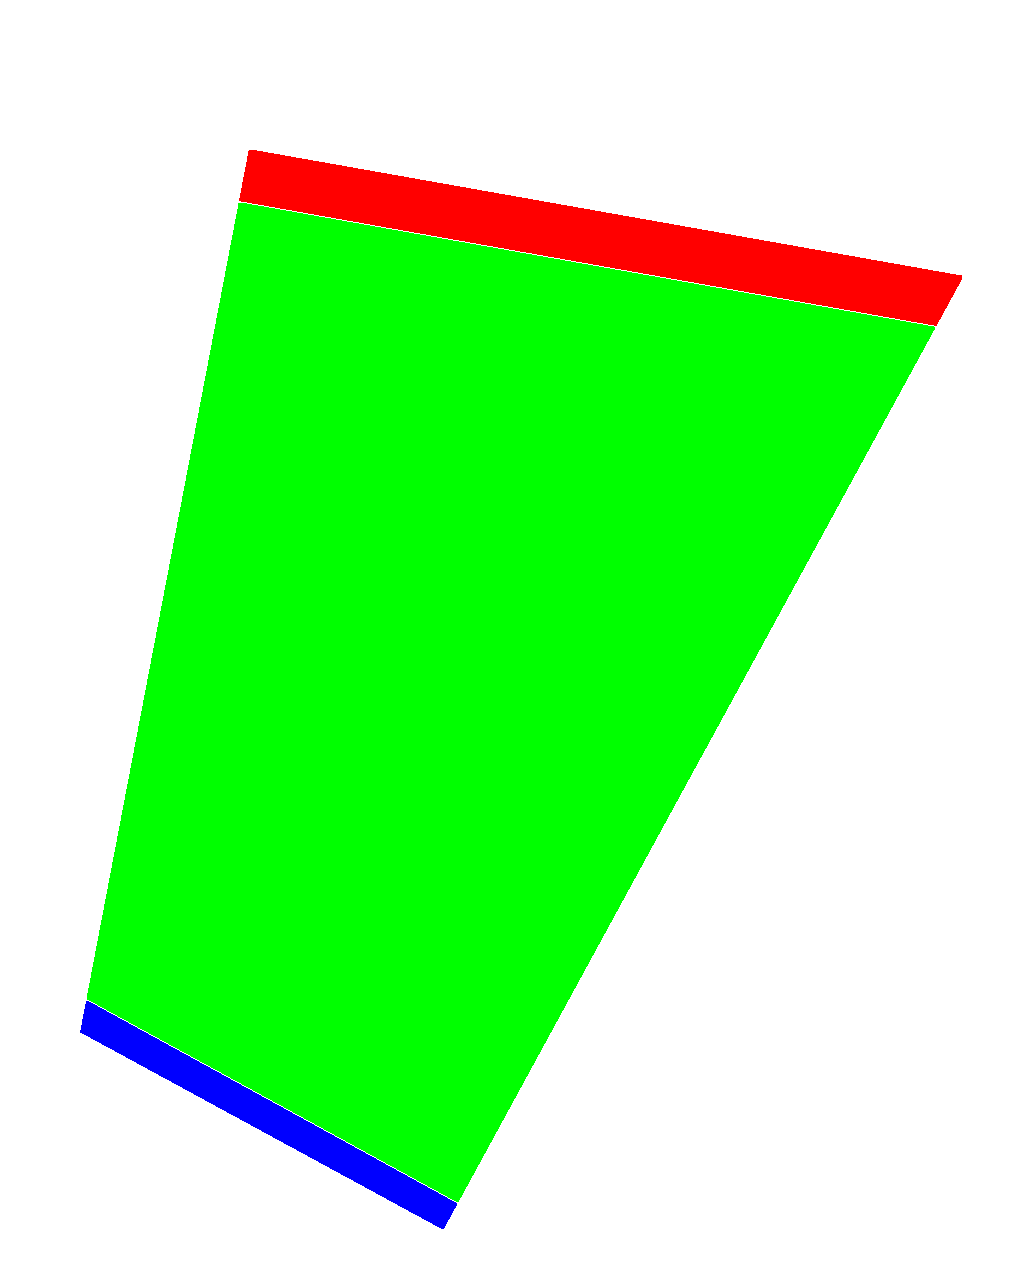
\includegraphics[width=0.4\textwidth]{segment_body_regions.png}} &
\fbox{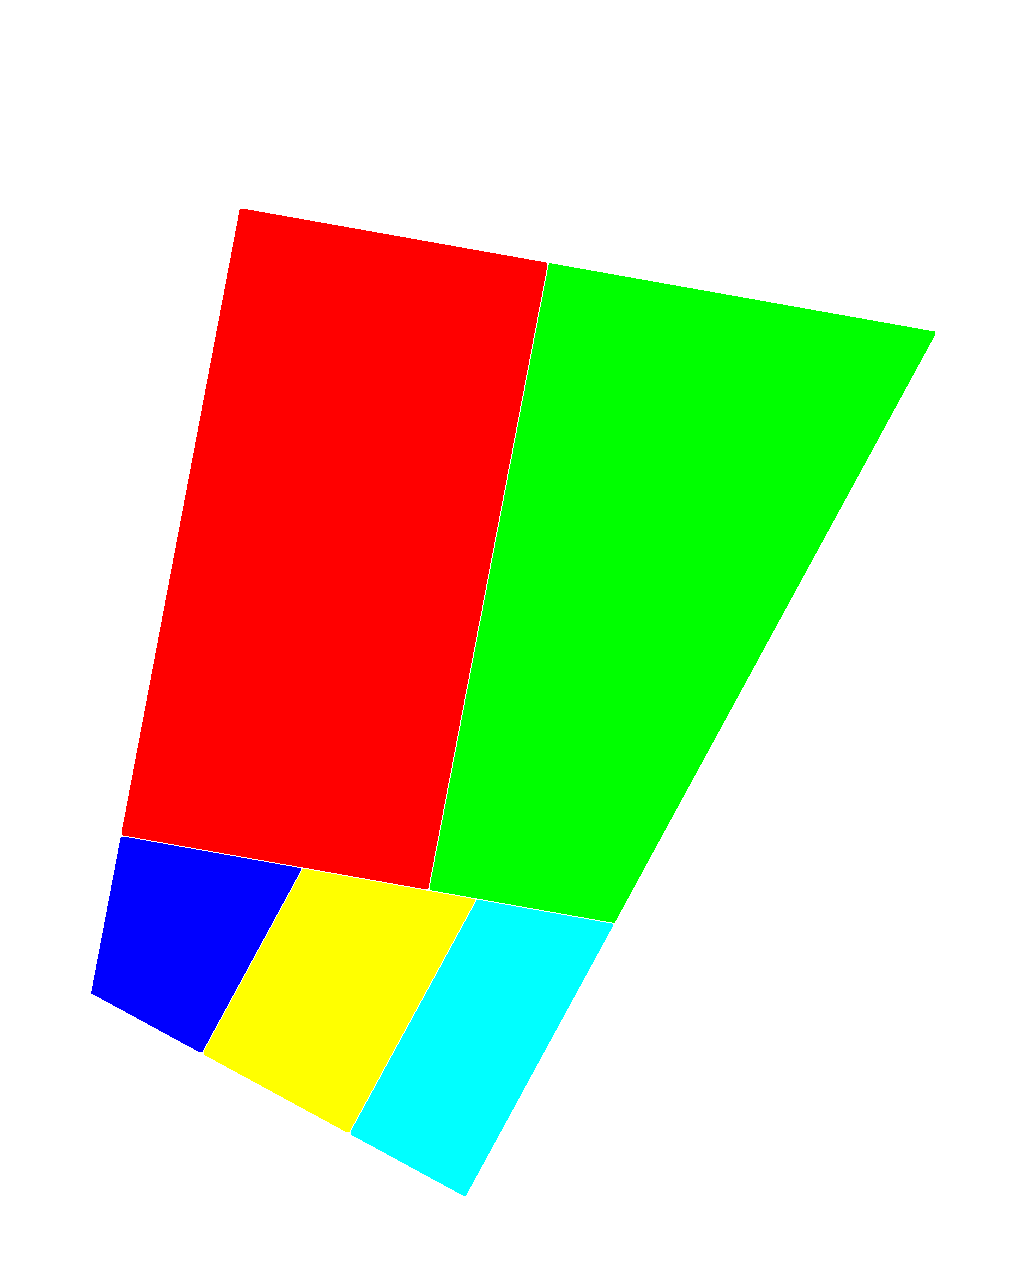
\includegraphics[width=0.4\textwidth]{segment_roof_regions.png}} \\
(a) & (b) \\
\fbox{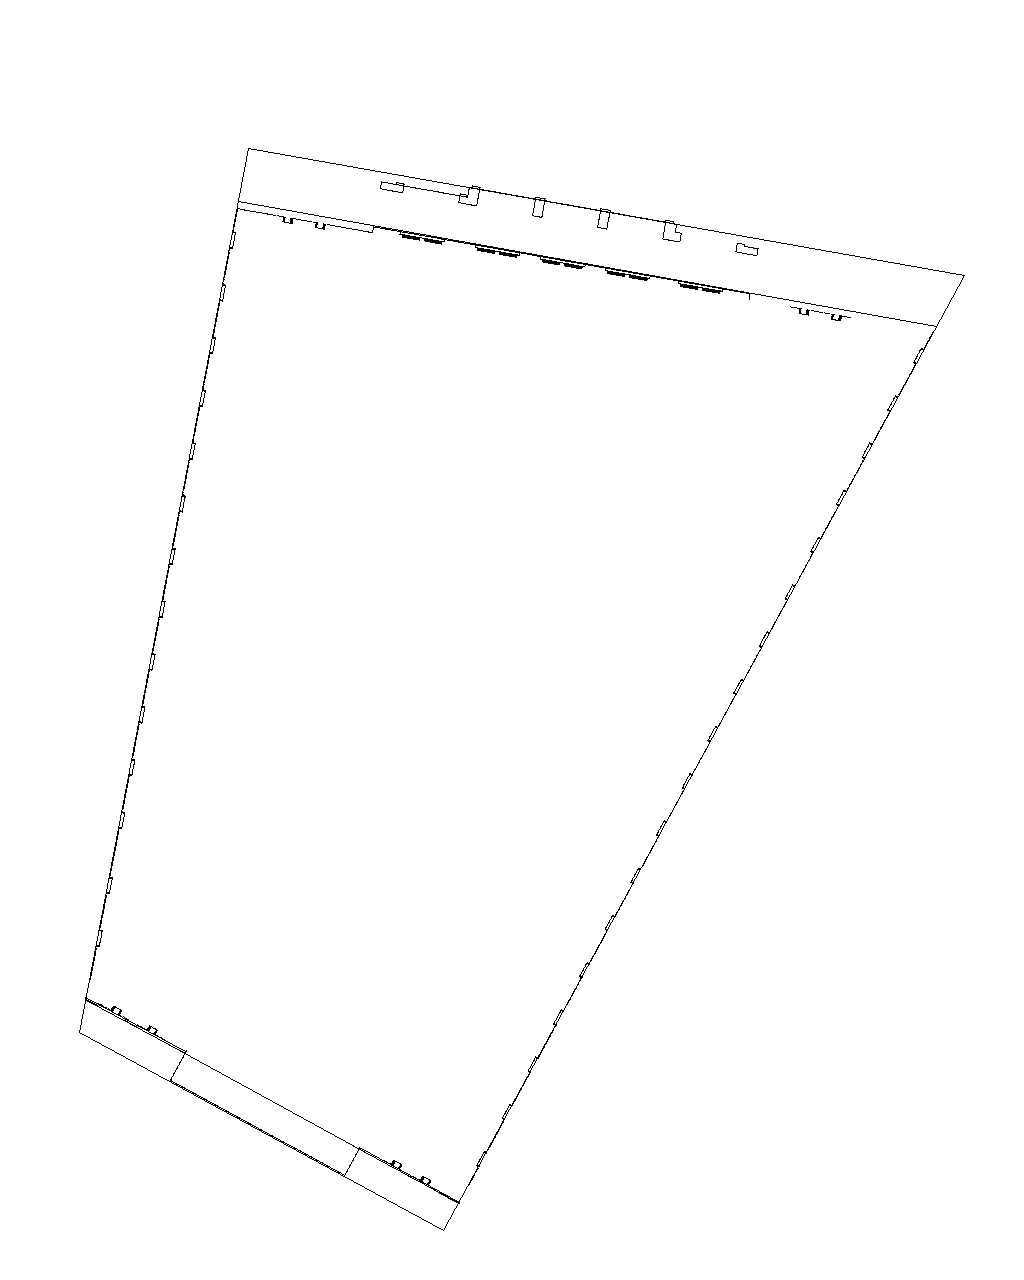
\includegraphics[width=0.4\textwidth]{integrate_body.png}} &
\fbox{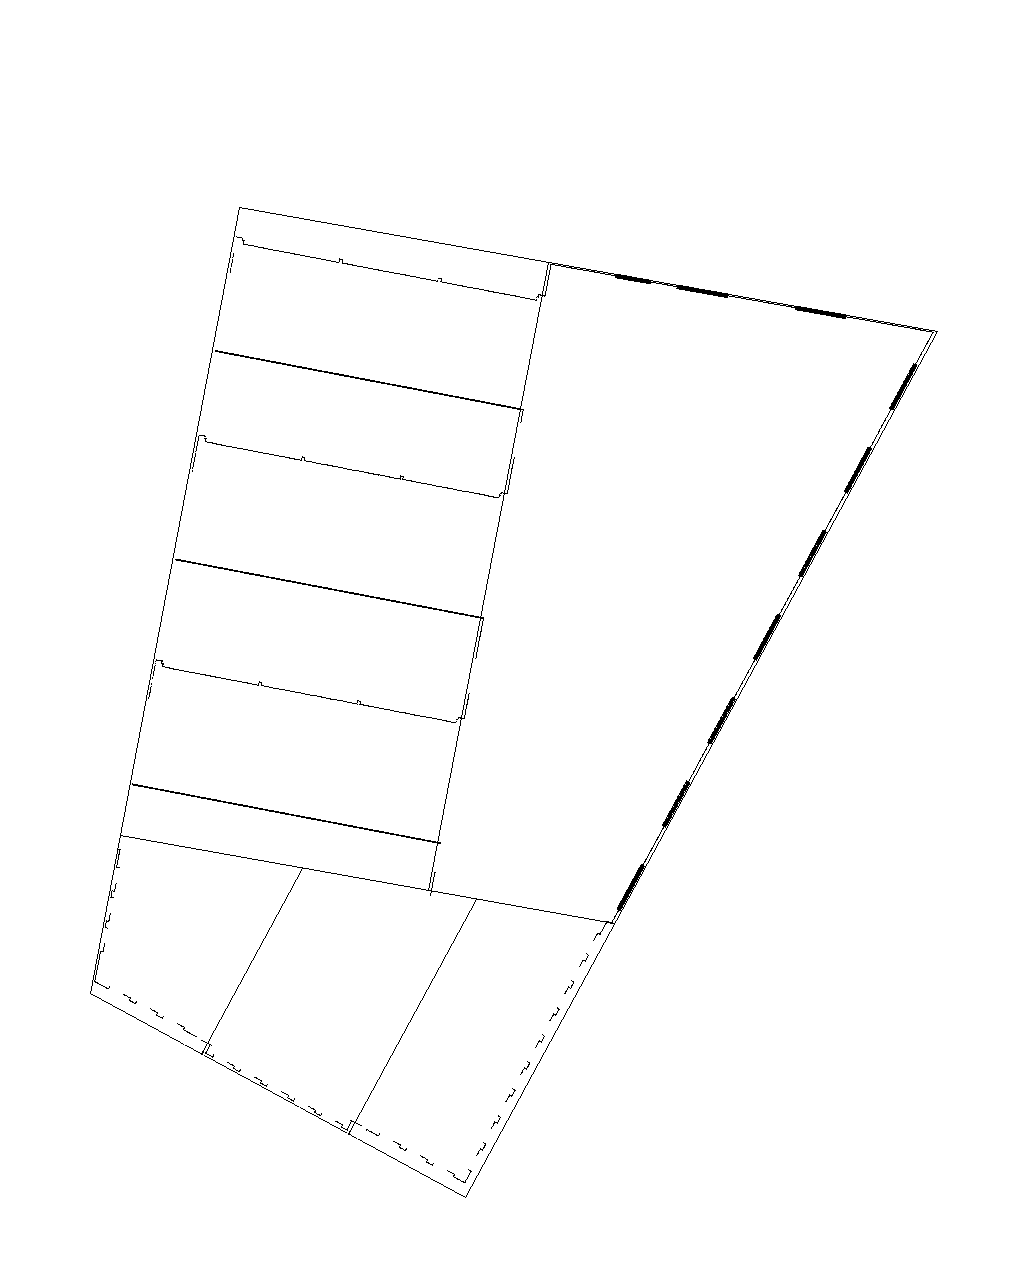
\includegraphics[width=0.4\textwidth]{integrate_roof.png}} \\
(c) & (d)
\end{tabular}
\end{center}
\caption{ Segmentation region computation:
      (a) the highlighted regions for \Figc{DS_Fig1};
      (b) the highlighted regions for \Figd{DS_Fig1};
      (c) the superimposed image of \Figc{DS_Fig1} with a sliced image from body section;
      (d) the superimposed image of \Figd{DS_Fig1} with a sliced image from roof section.}
\label{fig:DS_Fig1_1}
\end{figure}


% xxx -- backup
%However, manipulating the segmentation on sliced images
%also put the constraint on the segmented smaller images because
%we do not have the control on the size and resolution
%which have been fixed on the input 2D sliced images.
%We have tried both approaches, and found that
%the first approach does not slow down much but does offer
%greater flexibility on the manipulation of the segments.
%The second approach also works well on the segmentation.
%So either method is ok.

%% bottom-up division
To conduct the segmentation for the 2D sliced images,
we need to transform the separators computed from all major directions
into the common coordinate (with $y$-axis as the bottom-up direction).
Because the separators detected in bottom-up direction
are already in the common coordinate,
no transformation is needed for these separators
and the partitioning is straight-forward:
%
we first sort the indices $I$ of the bottom-up separators
in an ascending order.
The 2D slices projected along bottom-up directions
are grouped based on their indices against the sorted indices $I$.
For example, the group with index range of [$I_i$, $I_{i+1}$),
contains all 2D slices with indices greater than or equal to $I_i$
and less than $I_{i+1}$.
%
For the example of \Figc{syn_data},
The only detected separator (the ledger) as shown in \Figc{MS_Fig1}
divides the whole dataset into top (roof structure) and
bottom (body structure) parts.

%% other directions
The process becomes harder when we start the segmentation
on the 2D slices in the same group of height section.
First of all, all the separators detected in different directions
need to be brought to the common coordinate.
Each separator is transformed into
a line segment in the bottom-up projected image with the end points
representing the bounding positions.
The roof and body projected images are shown in
\Figa{DS_Fig1} and \Figb{DS_Fig1} respectively.
To compute the boundary for each segment,
the intersection points of
each line segment with other line segments need to be computed.
%
Given a line segment $L_i = P_0P_1$, represented by two end points $P_0$, $P_1$,
we can compute the intersection points of
$L_i$ with all other line segments.
%[ with the equation of intersection computation of two planar lines].
If the computed intersection point $P_i$ is falling outside of the image or
is far away from either $P_0$ or $P_1$,
$P_i$ is regarded as an invalid intersection point and is skipped.
When all the intersection points are checked,
we can obtain two special ones, $P'_0$ and $P'_1$,
which are the closest points to $P_0$ and $P_1$ respectively.
$P'_0$ and $P'_1$ represent the starting and ending points
of a wall or a facade of the underlying building.
After intersection points are computed for all line segments,
the segmentation image $I_s$ can be obtained.
\Figc{DS_Fig1} and \Figd{DS_Fig1} illustrate the computed segmentation images
for both body and roof sections.

With the segmentation images $I_s$,
we can compute each segment region for 2D slices projected in bottom-up direction.
To do this, we first build up a look-up table $T$
which maps a pixel point $(x, y)$ in $I_s$ to a region,
as shown in \Figa{DS_Fig1_1} and \Figb{DS_Fig1_1} for both body and roof.
Different regions are marked in different colors
and are assigned a unique region id.
For a given point $P(x, y)$ in each sliced images,
the region id for $P$ can be obtained from the look-up table $T$.
For example, for the roof sliced images,
all red pixels are mapped to the same region id in \Figb{DS_Fig1_1}.
The same situation is applied to green, blue, and other pixels.
After going through each point, a 2D sliced image from bottom-up direction
can be divided into segments.
The 2D sliced images for body and roof
with segmentation regions superimposed
are shown in \Figc{DS_Fig1_1} and \Figd{DS_Fig1_1}, respectively.
%%% segments on major planes other than bottom-up direction
%%%
For those 2D slices projected from normals of other major planes,
we carry out similar strategy for segmentation as that of bottom-up direction.



%% demonstration on 3D PCD
%% show the 3D image
To demonstrate the segmentation results on 3D dataset,
a similar process as 2D sliced image segmentation can be conducted.
For each 3D data point ${\bf P}(x, y, z)$,
we first compute its group in bottom-up direction
by comparing ${\bf P}$'s $y$ value (bottom-up direction) and
those heights from range indices.
%
Once the group is computed, with the segmentation image $I_s$,
we can further compute the region id for ${\bf P}$ by
obtaining its 2D projection point $P(x, y)$ in the image $I_s$.
%[ based on the equation [equation of the projection].
The region id for $P$ can be obtained from the look-up table $T$.
For the example in \Figc{syn_data},
there are totally 5 regions are identified for data points of roof
and 3 regions are located for body.
Hence the original point cloud of the building is
segmented into 8 segments as shown in \Fig{DS_Fig2},
where different segments are labeled with different colors.

\begin{figure} [htbp]
\begin{center}
\begin{tabular}{c}
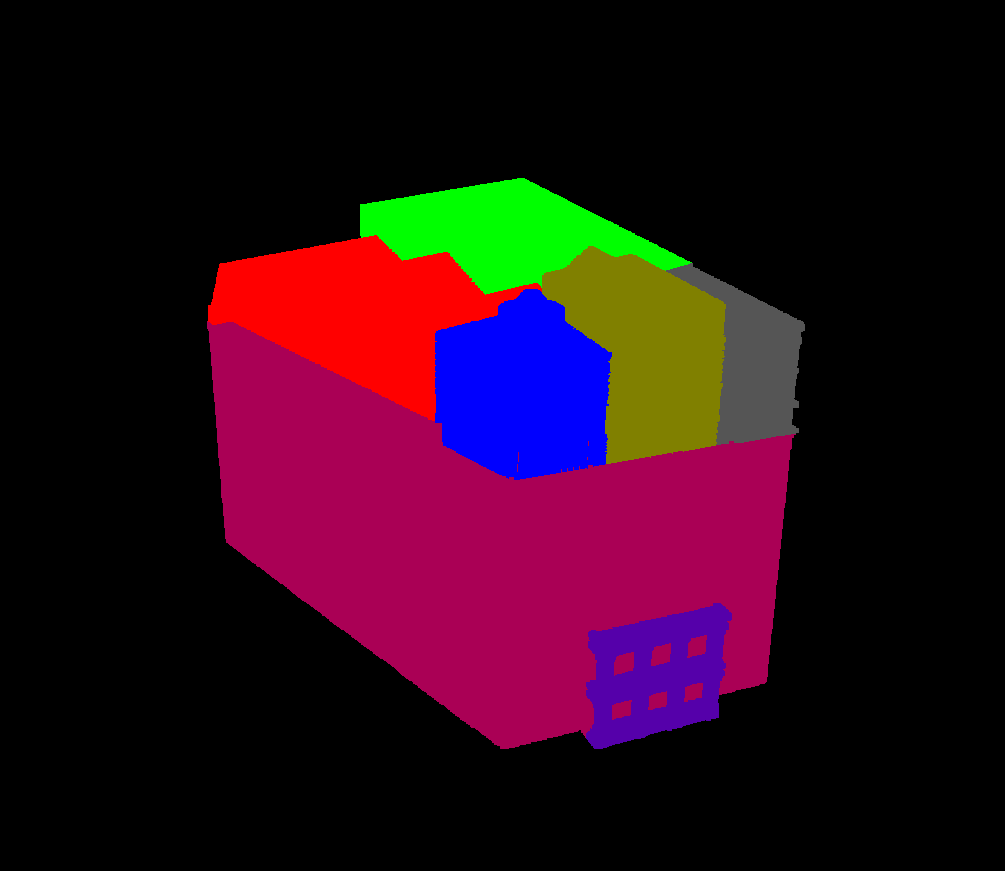
\includegraphics[width=0.75\textwidth]{cu_7.png}
\end{tabular}
\end{center}
\caption{The segmentation result for the point cloud in \Figc{syn_data}.}
\label{fig:DS_Fig2}
\end{figure}


%%%%% New Chapter %%%%%
%%%%% New Chapter %%%%%
\newchapt{Keyslice Detection}{chapt_key}{Keyslice Detection}

\label{sec:reconst}
Our 3D modeling algorithm is based on \emph{a priori} knowledge that
urban buildings can be created through a series of extrusion and tapering
operations on the salient cross-sections contained in the keyslices.
The key step for successful modeling is identifying these salient cross
sections upon which the extrusion and tapering operations will apply.

Buildings generally are equipped with windows and doors which should not
be considered as salient feature for keyslices.
Therefore, data points corresponding to windows and doors
should be discarded to avoid possible side-effects
during the keyslice computation.

\section{Window Detection}
\label{sec:wdd}

Windows and doors are important features for buildings to be modeled.
Moreover, accurate computation of the extrusion structures
depends on these information.
Without knowing the marked location as window part,
extra keyslices may be computed and hence lead to excessive extrusion operations.
Image-based window detection has been widely conducted in
\cite{WDD_LN,WDD_TKKJ}.
Essentially, the 2D window regions are extracted by exploiting the properties
of building structures, such as shape and symmetry.
The estimation of the depth for the extracted 2D windows is computed
by using matches for the linear features within the extracted
window in two or more ground views.
However, the estimation is not reliable due to perspective projection.
Some window detection methods on 3D data have also been proposed in
\cite{WDD_SV,WDD_BBH}.
A constrained surface fitting based algorithm
is proposed to fit parametric models of doors on point cloud in \cite{WDD_FF}.
This method assumes that the data have been segmented
and requires relatively high density data around the window area.
Pu and Vosselman use a triangulation-based method
to detect the boundaries of sparse regions within a building facade
and then fit rectangles to the resulting region to compute windows \cite{WDD_PV}.
However, this method needs to improve its accuracy when background noise exists.

\begin{figure}[htbp]
  \centering
  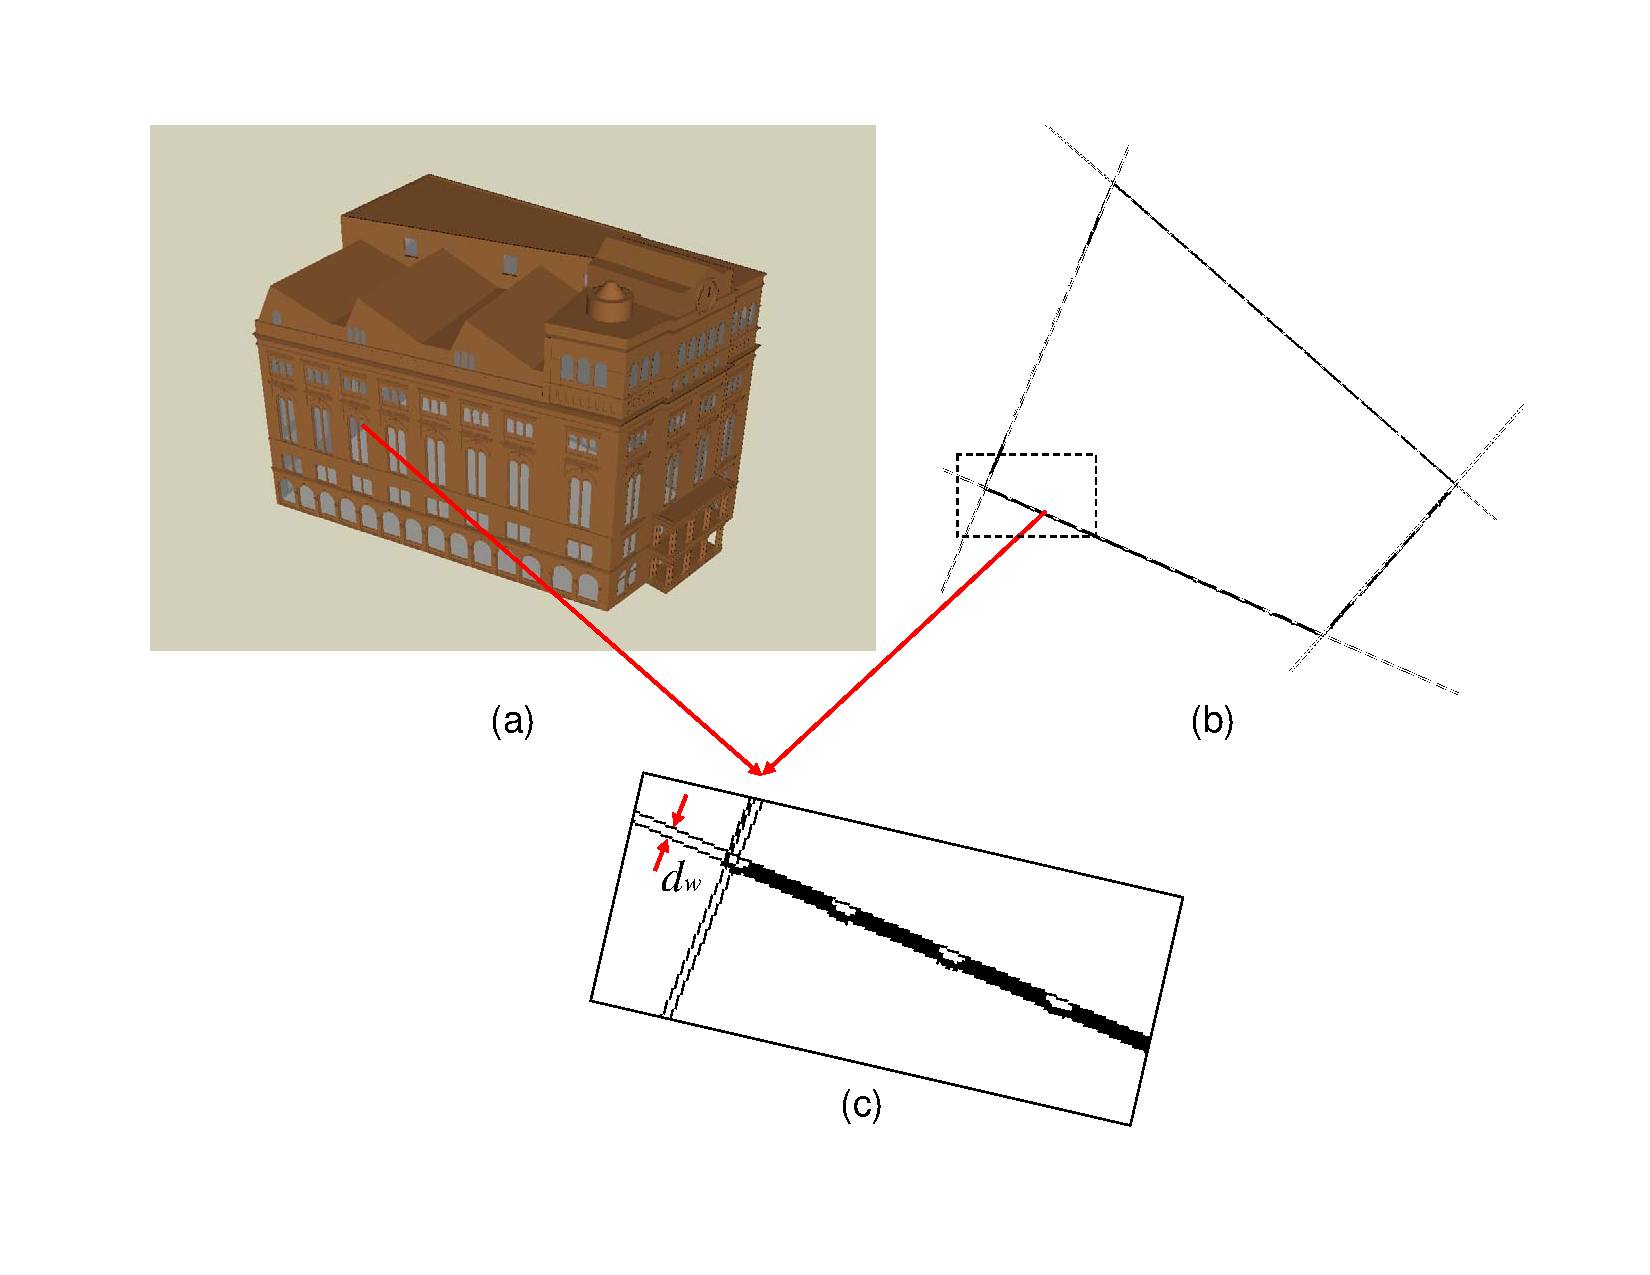
\includegraphics
      [width=\textwidth]
      {model_win_comp.pdf}
      \caption{The depth computation of the windows/doors:
      (a) the window on the original model;
      (b) the projected slice extracted from bottom-up direction;
      (c) the close-up view of the parallel lines and the distance $d_w$. }
      \label{fig:WD_Fig1}
\end{figure}

%[show a figure with unnecessary keyslice? how?]
The information we want to compute for windows and doors includes
both the location and the depth.
The depth is computed based on the observation that two parallel lines can be detected
when viewing from the bottom-up direction as shown in \Figc{WD_Fig1} .
For two parallel lines $L_1: y = mx + c_1$ and $L_2: y = mx + c_2$,
% as shown in Fig1,
% http://www.askiitians.com/iit_jee-Straight_Line/Distance_between_two_parallel_lines
the distance $d_w$ is computed with the following equation,
\begin{equation*}
d_w = \frac{|c_1 - c_2|}{\sqrt{1 + m^2}}
\end{equation*}

%[Fig1: show the window thickness detection image, two parallel lines are drawn]
%[Fig2: show the projected windows/doors slice]

\begin{figure}[htbp]
  \centering
  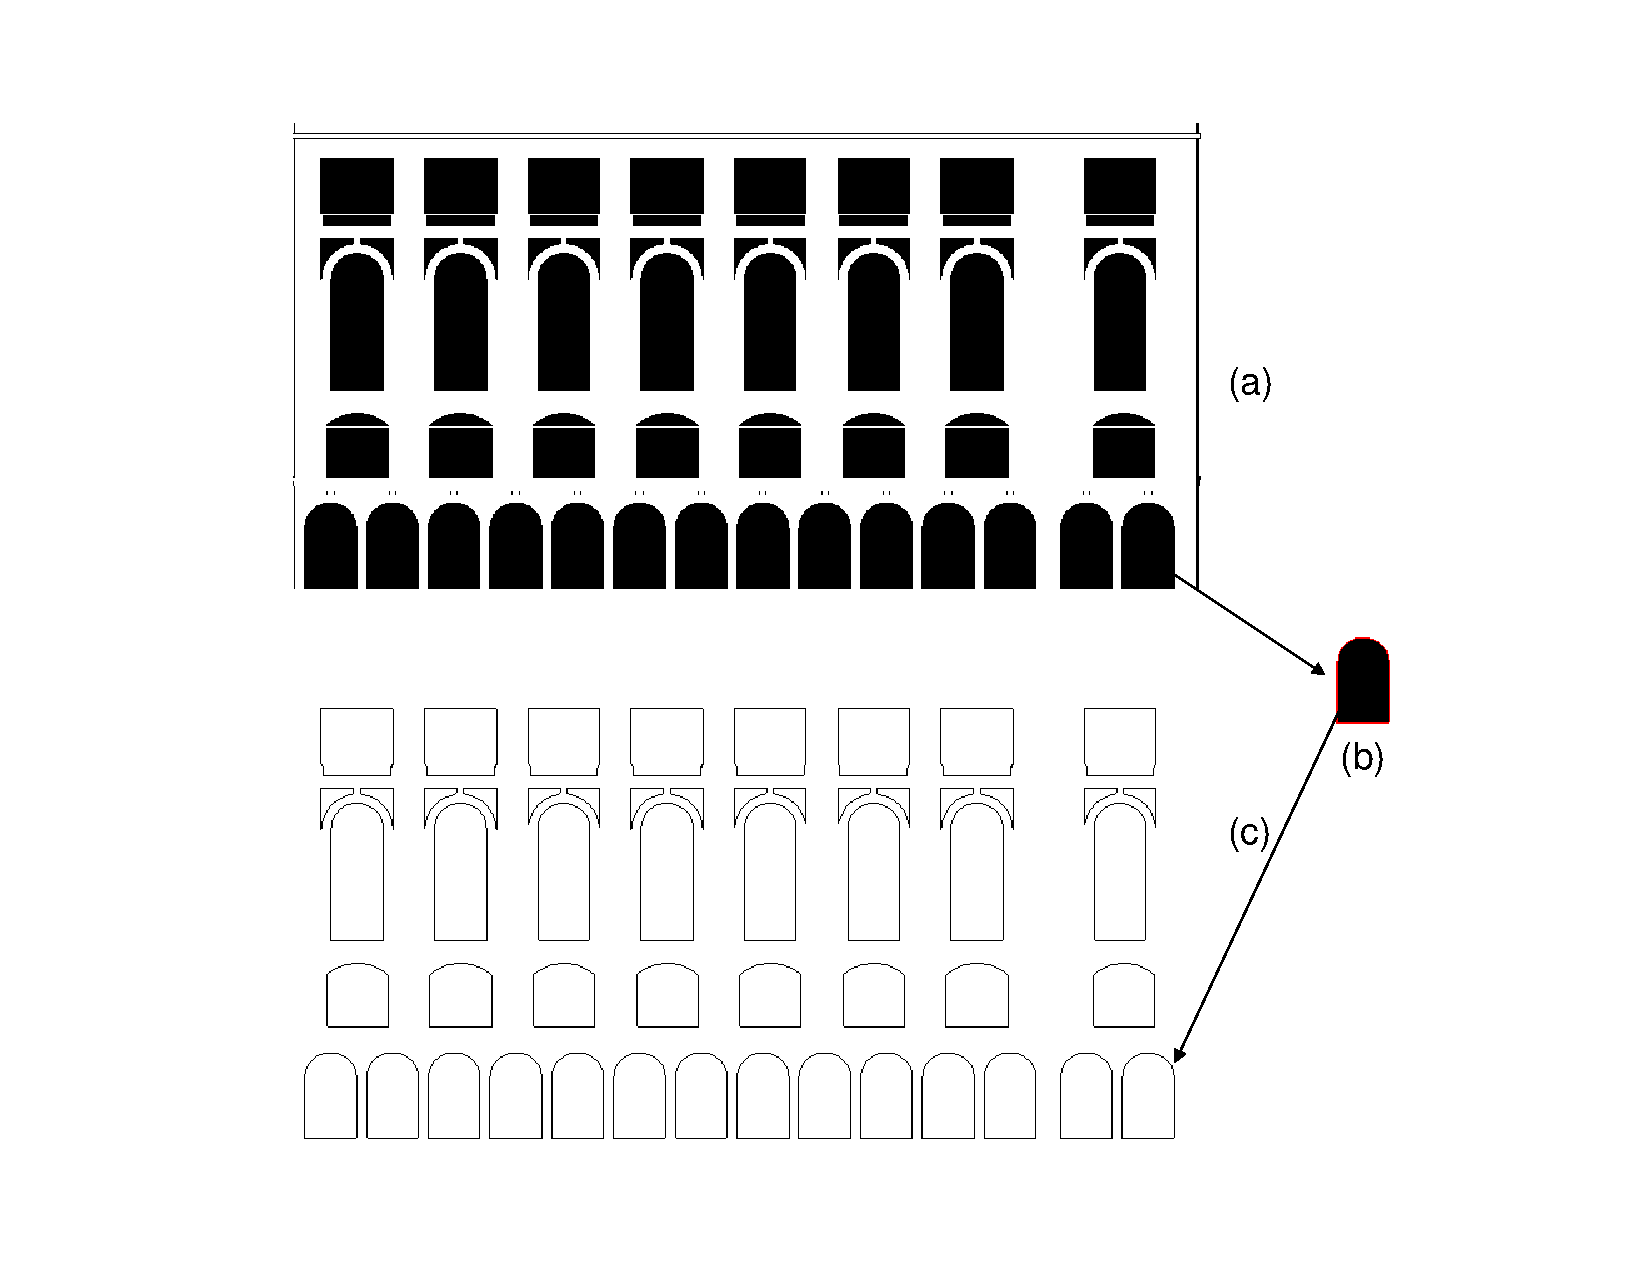
\includegraphics
      [width=\textwidth]
      {window_result.pdf}
      \caption{The window information: (a)the projected windows slice;
      (b) the most bottom-right window extracted from (a) with BPA contour in red;
	(c) the contours of windows computed from (a).}
      \label{fig:WD_Fig2}
\end{figure}

%%% xxx -- not clear
Once the distance $d_w$ is computed,
we can obtain the windows/doors image by projecting the data points
between $L_1$ and $L_2$ onto a slice image as shown in \Figa{WD_Fig2}.
There are multiple window structures in the same projected slice image.
We can use the same strategy as separator detection described in \Sec{sd}, that is,
kernel based connected component method, to isolate each window for processing.
\Figb{WD_Fig2} shows a window extracted as a connected component and BPA algorithm was applied
to obtain the contour in red.
After walking through the image shown in \Figa{WD_Fig2} for all the connected components
and applying BPA on them,
the final results show all the detected window contours as depicted in \Figc{WD_Fig2}.
These contours will be used to compute window mask images
and project windows and doors onto the final model.

The above window detection is for synthetic dataset since clean result can be obtained.
For real dataset, due to noise and missing data,
the computed window images are usually not able to
be processed using the above method and manual efforts
are needed to assist the computation.
\Fig{WD_Fig3}(a)-(c) show the consecutive projected images with window structures.
\Fig{WD_Fig3}(d) shows the integrated image from slice (a) to (c).
As we can see, some data are missing around the window section.
We have to enhance the image by manually marking the locations
of these window structures as shown in \Fig{WD_Fig3}(e).
With the assistance of user interaction, we can obtain the final window
structure as shown in \Fig{WD_Fig3}(f).

\begin{figure}[htbp]
\begin{center}
\begin{tabular}{cc}
\fbox{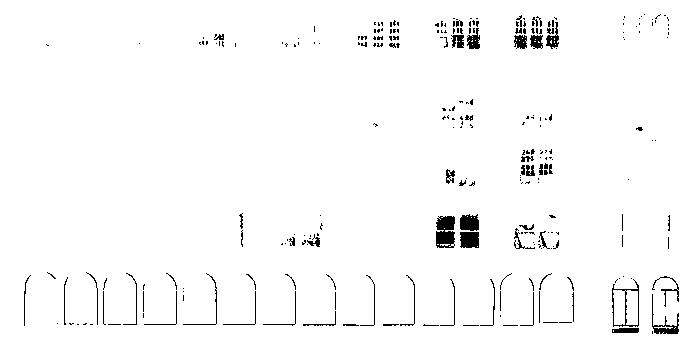
\includegraphics[width=0.45\textwidth]{image_slice_0058.png}} &
\fbox{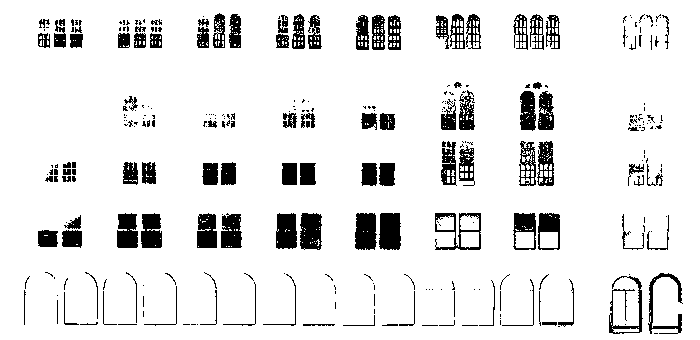
\includegraphics[width=0.45\textwidth]{image_slice_0059.png}} \\
(a) & (b) \\
\fbox{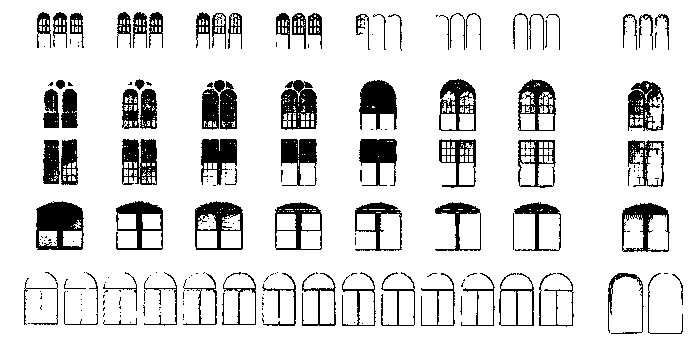
\includegraphics[width=0.45\textwidth]{image_slice_0060.png}} &
\fbox{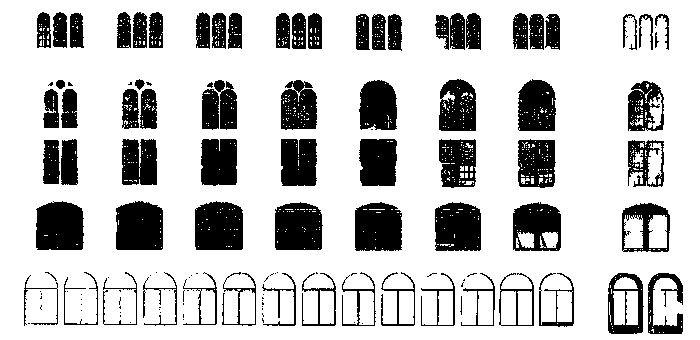
\includegraphics[width=0.45\textwidth]{image_slice_0058_0060.png}} \\
(c) & (d) \\
\fbox{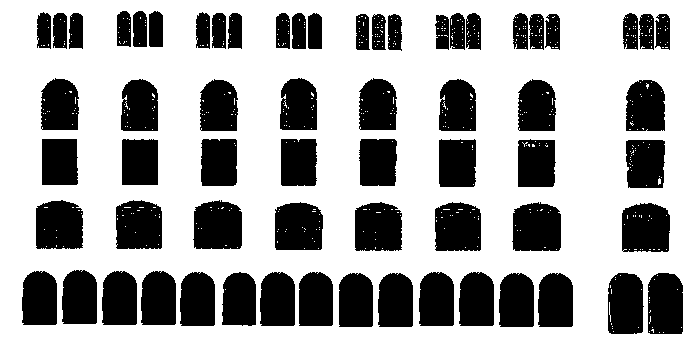
\includegraphics[width=0.45\textwidth]{image_slice_windows.png}} &
\fbox{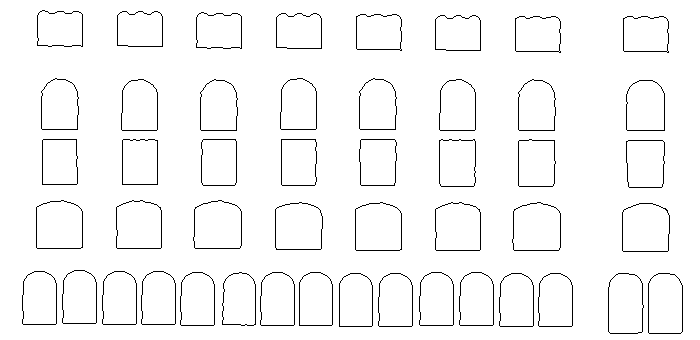
\includegraphics[width=0.45\textwidth]{image_slice_windows_contour.png}} \\
(e) & (f)
\end{tabular}
\end{center}
\caption{
Window detection for real dataset: (a) - (c) are consecutive slices;
(d) integrated slice from (a) to (c);
(e) manually enhanced image for (d);
(f) window structure computation from (e).
}
\label{fig:WD_Fig3}
\end{figure}


\subsection{Windows Mask Image Generation}

Windows and doors detection have been discussed in \Sec{wdd}.
If there is no windows or doors structures detected in the current PCD,
this step is skipped.
However, when windows or doors are detected,
the data points corresponding to these structures in cross-section images
should not be taken into account for keyslices computation.
This is to ensure that no keyslices are generated
due to curve or any geometry shapes introduced by windows or doors.

To generate the mask images, the information about windows and doors,
including width, height, depth are needed, which has been computed previously.
Let $\{x_{min}, x_{max}, y_{min}, y_{max}, z_{min}, z_{max}\}$
be the bounding box $w_{box}$ of a window $w$,
where $x, y, z$ are corresponding to width, height and depth directions.
The $w_{box}$ is transformed to bottom-up direction,
with $x, z$ defining the rectangle location of the window,
and with $y$ defining the height range for $w$.

\begin{figure}[htbp]
\begin{center}
\begin{tabular}{cc}
\fbox{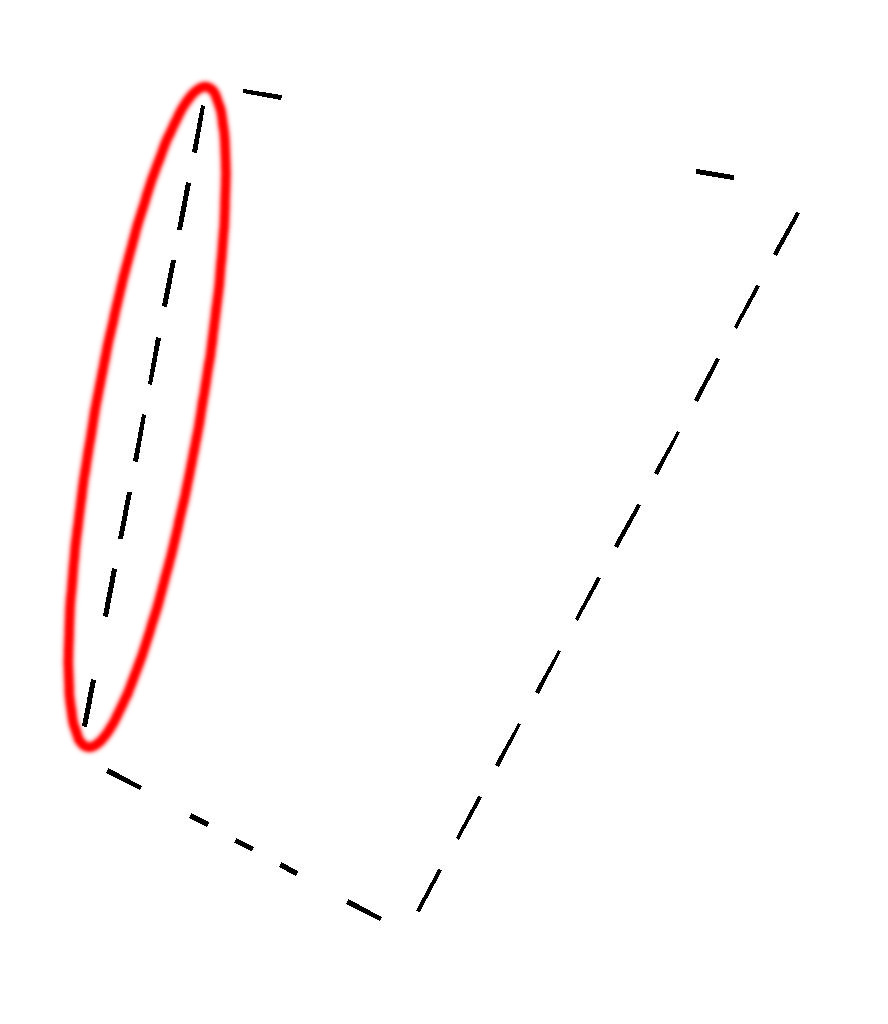
\includegraphics[width=0.4\textwidth]{window_mask_1.jpg}} &
\fbox{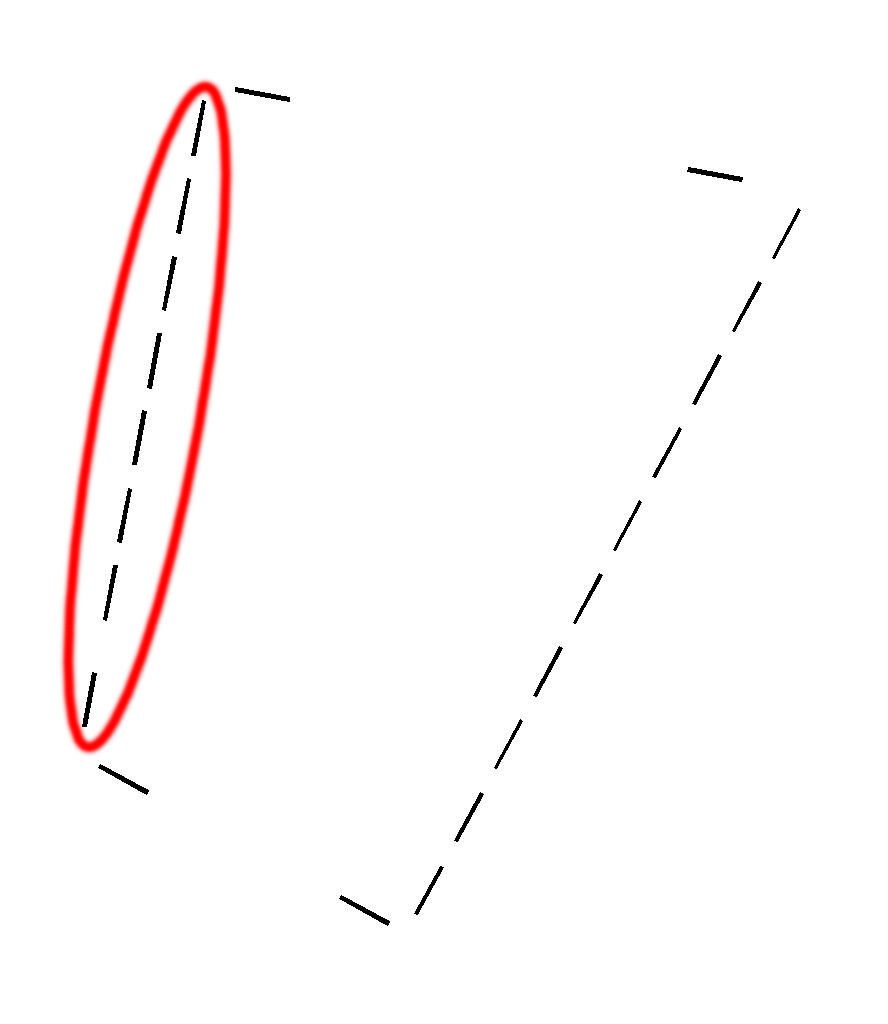
\includegraphics[width=0.4\textwidth]{window_mask_2.jpg}} \\
(a) & (b)
\end{tabular}
\end{center}
\caption{The window mask images:
         (a) the mask image corresponding to height range of bottom windows;
	 (b) the mask image corresponding to height range of upper windows.}
\label{fig:WD_Fig4}
\end{figure}

After computing the mask information for all windows,
the mask images can be generated by fusing all the window information.
\Fig{WD_Fig4} shows couple of mask image examples
for different height range of the cross-section slices.
The regions circled in red are corresponding to
the locations of the windows in \Figa{WD_Fig2} in different height range.

Once the mask images are obtained,
a simple bit-and operation with the original 2D slice image
eliminates the data points corresponding to windows or doors.
That is, $I_n = I \, \& \, I_w$, where $I$ is a 2D slice, $I_w$ is the mask image,
and $I_n$ is the updated 2D slice with window or door data points removed.
The updated $I_n$ slices are used for keyslice detection.

\section{Keyslice Detection With Distance Measurement}
\label{sec:ksd}

An intuitive way for keyslice detection is to
compute the similarity between the sliced images.
In other words, the sliced images are clustered into different groups
based on the similarity among them.
Similarity measure has been extensively studied in the image registration
research community \cite{IR_Brown, RE_WWLZ}.
Recently, Zitova and Flusser conducted an survey on
image registration and they identified two major research methods
for similarity measure of 2D images, i.e.,
area based methods and feature based methods \cite{IR_ZF}.
Area based methods are also called correlation-like methods or
template matching methods, which compute similarity of images
without attempting to detect salient features or objects.
The feature based methods, on the other hand, aim to find
the pairwise correspondence of features between two images based on
spatial relations or various descriptors of features represented
by control points, such as end points or centers of line features,
centroid of regions, etc.

The area based methods are computational efficient
but they usually can only be applied on binary or gray-scale images.
The feature based ones are computational complex but more powerful
and can be applied to images obtained using different sensors,
such as multi-modal image registration.
Because our 2D sliced images for similarity measure are pure binary images,
and are projected from the same 3D range data,
the area based methods are more efficient and appropriate.

For area based methods, usually a predefined window or even the entire image
are used for the similarity measure.
The classical measurement for area based method is the cross
correlation as presented in \cite{DIP_Pratt}.
However, this method becomes very time consuming when the size of window
increases in order to capture the global relations between images.
To address this issue, the phase correlation methods
based on the Fourier Shift Theorem
in frequency domain are proposed.
The phase correlation was originally proposed for the registration of translated images.
It can be combined with log-polar mapping of the spectral magnitude
to handle rotation and scale transform of images.
Wolberg and Zokai \cite{DIP_WZ} showed such combination power to register
affinely distorted images.
They used a variation of Levenberg-Marquardt nonlinear least squares
optimization method for iterative estimation of perspective deformation.
In addition to correlation methods,
the mutual information (MI) methods, originating from the information
theory, are proposed to measure statistical dependency between two images.
MI methods are particularly suitable for images acquired from different modalities.
Viola and Wells \cite{DIP_VW} applied MI on magnetic resonance images
and employed the coarse-to-fine speed up using the gradient descent
optimization method.

Although these approaches are very powerful, they are time consuming and
not suitable for our scenario.
Huttenlocher {\it et al.} \cite{IR_HKR} proposed Hausdorff distance (HD)
based similarity measure for binary images.
This method is computationally efficient and
can handle images with perturbed pixel locations,
which outperforms the correlation methods.
We adopted a light-weighted global and efficient key image detection approach
based on distance function similar to
Hausdorff distance as the similarity measure.
Let $P_r(x_r, y_r)$ be a data point in a reference image and
let $P_i(x_i, y_i)$ be a data point in a new observed image $I$.
The distance of image $I$ to reference image $I_r$ is defined as:
\begin{equation}
d_H(I, I_r) = \sum_{i=0}^Nd_{min}(P_i, I_r)
\label{eq:hd}
\end{equation}
where $d_{min}(P_i, I_r)$ is the minimum distance from data point $P_i$
in image $I$ to the reference image $I_r$.
Alternatively, we can also define the distance, $d_H(I_r, I)$,
from reference image $I_r$ to a new observed image $I$, using \Eq{hd}.
These two distances are usually not equal to each other.
As a rule of thumb, one can choose
$d_{HD} = \text{MAX}\{d_H(I, I_r), d_H(I_r, I)\}$ as the distance function.
To compute the keyslices, a threshold $\tau_d$ is used for  $d_{HD}$.
If $d_{HD} < \tau_d$, the two images $I$ and $I_r$ are considered
similar to each other.
Otherwise, a keyslice image is found and $I_r$ is updated with $I$,
the new keyslice image.


\begin{figure}[htbp]
\begin{center}
\begin{tabular}{cc}
\fbox{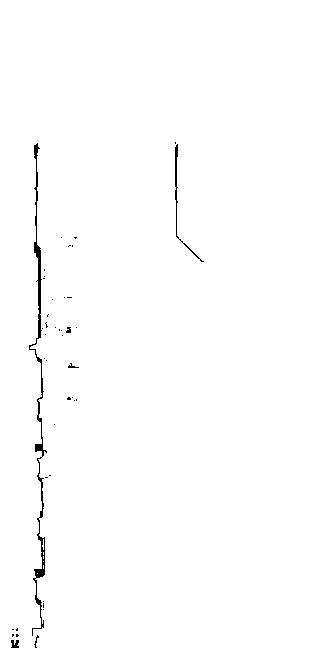
\includegraphics[width=0.3\textwidth]{image_slice_lr_0580_0590_half.jpg}}
\fbox{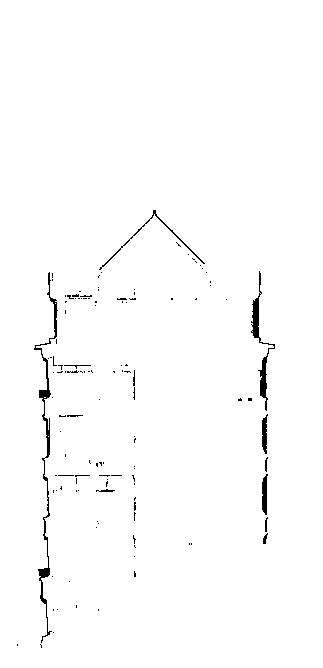
\includegraphics[width=0.3\textwidth]{image_slice_lr_0830_0842_half.jpg}} &
\fbox{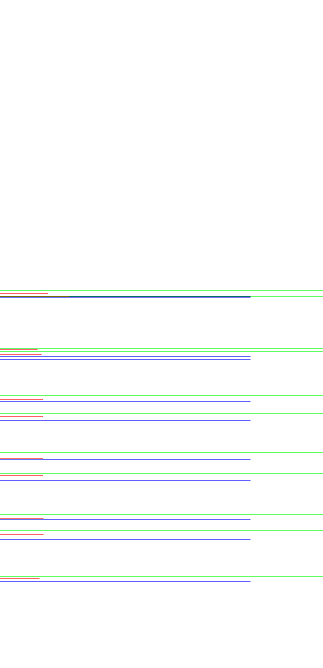
\includegraphics[width=0.3\textwidth]{curvature_center_lines_old_half.jpg}} \\
(a) & (b)
\end{tabular}
\end{center}
\caption{Curvature-based key slice detection:
(a) a partial set of two 2D sliced images from the orthogonal direction (side
view). The complete set will be used to extract the keyslices shown in
\Fig{keyslices}.
(b) the average curvatures detected over all of the sliced images along the
orthogonal direction.}
\label{fig:HT_BPA_Curvature}
\end{figure}

%%% implementation details? xxx - for example, 0.9% data for comparison.
%%%

\section{Keyslice Detection With Curvature}
The accuracy of the keyslices detected by the distance measurement
is closely tied to threshold $\tau_d$.
Small $\tau_d$ leads to more accurate models and will require more time and
space to compute and store the results.
When the threshold $\tau_d$ is relatively large, potential keyslices which
contain salient structures may be missed.
Therefore, there is a trade-off between model accuracy and time-space
efficiency.

We can improve the model accuracy by computing curvature information
as a complementary criteria for keyslice detection.
The idea is based on the observation that the keyslices are generally
located at large curvature changes along 2D slices extracted in the orthogonal
direction (e.g., side view), as shown in \Figa{HT_BPA_Curvature}.
Therefore, instead of computing the difference between two images directly,
we compute the curvatures of orthogonal 2D slices,
map the positions of curvature extrema back to cross-sections
in the original set of volumetric slabs,
and mark these cross-sections as keyslices.

%%% Figure of the tapering template.
\begin{figure}[htbp]
\begin{center}
\begin{tabular}{c}
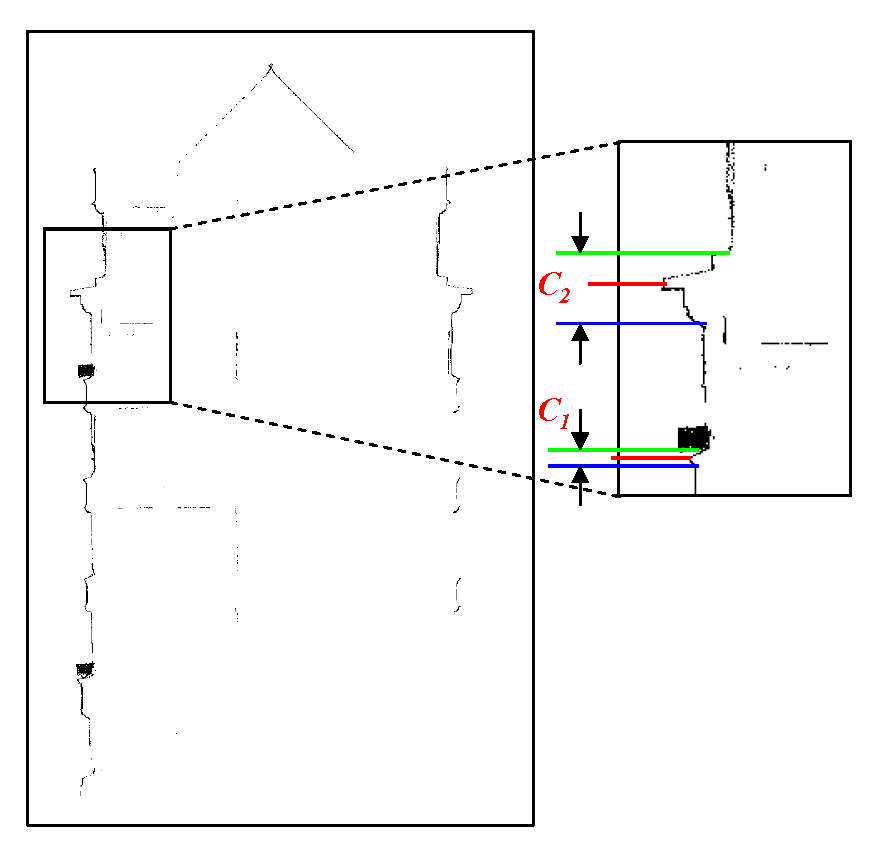
\includegraphics[width=0.5\textwidth]{curvature.png}
\end{tabular}
\end{center}
\caption{ Curvature based key slice detection. }
\label{fig:KSD_Curv}
\end{figure}
%%% End of Figure

In the close-up view of a small region as shown in \Fig{KSD_Curv},
two curvatures, $c_1$ and $c_2$, are
computed in this small region. The red, blue and green lines indicate the locations
of the center, the starting and the ending of a curvature.
As a matter of fact, there is a third curvature computed around the
black box sitting on top of the green line of the curvature $c_1$.
However, this third one should not be considered as a real curvature
in that the black box is due to an air conditioner during the data acquisition process,
which means it is not a part of the building.
The third curvature, or {\it outlier curvature},
needs to be removed from the set of real curvatures.
Based on the fact that these outlier curvatures exist only in a few 2D slices,
we can exclude them by counting the number of appearance for each curvature.
Only those curvatures appears in most of the 2D slices are kept for further computation.

Once the real curvatures are obtained, they can be used as a complemental way of
 distance measurement for keyslice detection.
Each curvature $c$ is mapped to a set $s$ of original 2D cross-sectional
slices, $i,\ldots,j$, where $i$ and $j$ are corresponding to the starting and
the ending locations of $c$. After this, the set $s$ is checked whether
it contains any keyslice or not.
If a keyslice $k$ has been marked in $s$ by distance measurement,
nothing needs to be done and this curvature $c$ is discarded.
On the other hand, if $s$ contains no keyslice, $i$ and $j$ will be marked as
two new keyslices to keep the salient feature identified by this curvature $c$.
The combination of distance measurement and curvature inference
ensures that the salient structures of a building will be preserved.
\Fig{keyslices} depicts the keyslices derived from the uniform slices
given in \Fig{slice_slab}.

\begin{figure}[hbtp]
\begin{center}
\begin{tabular}{c}
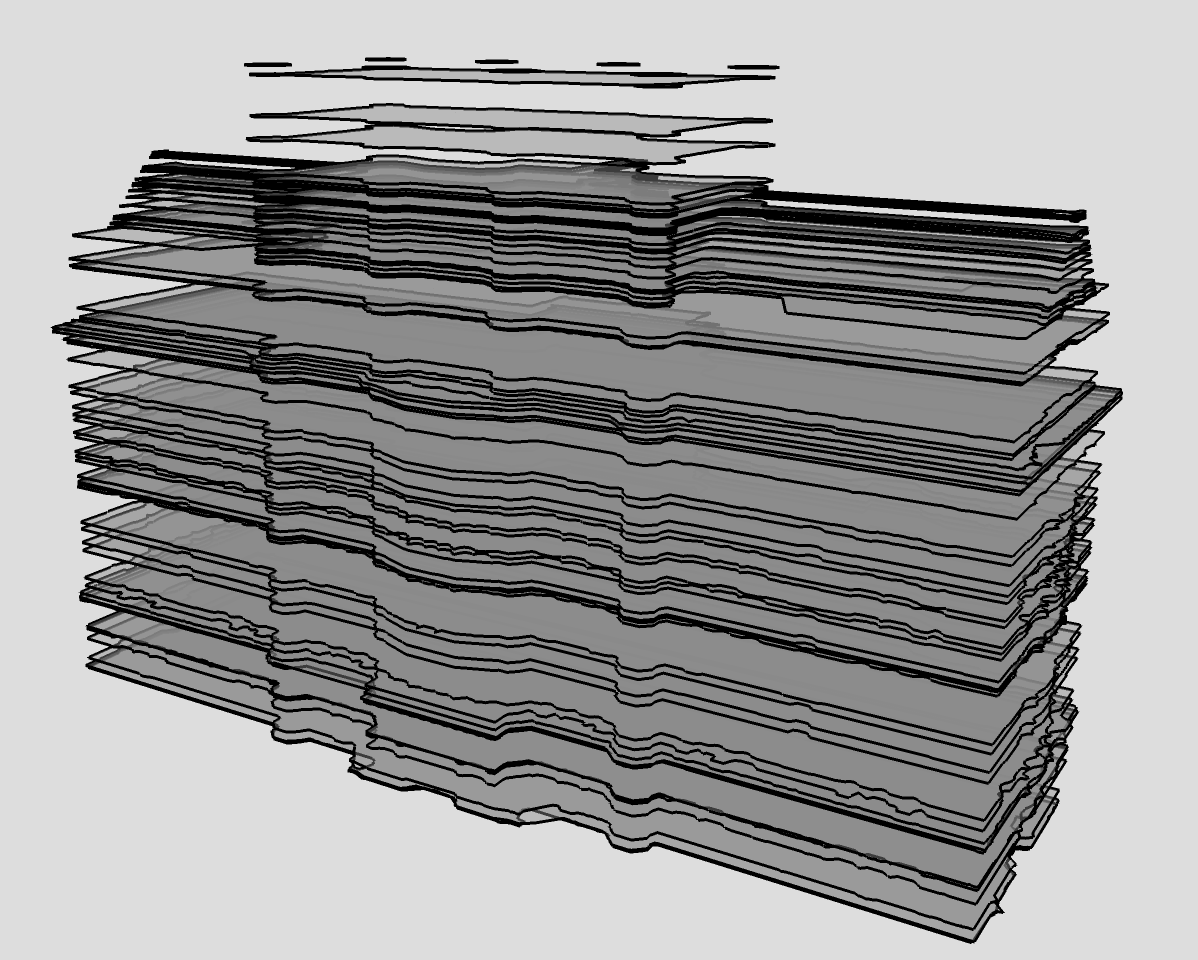
\includegraphics[width=0.7\textwidth]{keyslice_wireframe.png}
\end{tabular}
\end{center}
\caption{Keyslices derived from the input in \Fig{slice_slab}.}
\label{fig:keyslices}
\end{figure}

\section{Algorithm Analysis of Keyslice Detection}
\label{sec:aa_kd}

The proposed keyslice detection is summarized in Algorithm \ref{alg.KSD}.
The algorithm consists of two independent functions.
The function {\it Distance()} conducts
distance measurement based keyslice detection.
And the function {\it Curvature()} carries out the
curvature based keyslice detection.
A lookup table $t$ is computed in the function {\it lookup()}.
This lookup table is used to store for each pixel $p$,
the distance to the nearest data point in the reference image $I_r$ or $I_i$.
If $p$ itself is a data point, the distance is 0.
The complexity of constructing $t$ is bounded by $O(n)$,
where $n = w * h$, and $w$ and $h$ are the image width and height respectively.
The function {\it dis()} is basically doing hashing computation on $t$,
which takes only $O(1)$ run time.
The function {\it avg()} computes the average of $d_1$ and $d_2$,
i.e., $(d_1 + d_2) / 2$, which takes $O(1)$ time complexity.
The function {\it append()} appends a new index value $i$
to the linked list $L$, which takes $O(1)$ time complexity too.
Because there are total $K$ sliced images, and $K$ is a constant value,
the complexity of the function {\it Distance()} which composes of
the above functions takes $O(K*n) = O(n) $ for the computation.

\begin{algorithm}
\caption{The Keyslice Detection Algorithm}
\label{alg.KSD}
\begin{algorithmic}[1]
\Procedure {Distance}{$I$, $K$}
  \State $L \leftarrow \emptyset$  \Comment{vector to store the indexes of keyslices}
  \State $I_r \leftarrow I_0$
  \For { $i \leftarrow 1, K-1 $}
    \State $t \leftarrow lookup(I_r); d_1 \leftarrow dis(I_r, I_i, t) $
    \State $t \leftarrow lookup(I_i); d_2 \leftarrow dis(I_i, I_r, t) $
    \State $d_{HD} \leftarrow avg(d_1, d_2) $ \Comment {average distance}
    \If { $d_{HD} > \epsilon $}
       \State $I_r \leftarrow I_i$  \Comment{update the reference image}
       \State $ append(L, i) $
    \EndIf
  \EndFor
  \State \textbf{return} $L$
\EndProcedure

\Procedure {Curvature}{$I$, $K$}
  \State $L \leftarrow \emptyset$  \Comment{vector to store the indexes of keyslices}
  \State $V \leftarrow 0$ \Comment {initialize the counter to 0}
  \For { $i \leftarrow 0, K-1 $}
     \State $\bigcup{C} \leftarrow curv(I_i)$ \Comment{curvature computation on image $I_i$}
     \State $\bigcup{c} \leftarrow mapping(\bigcup{C}) $ \Comment{mapping the curvature to indexes}
     \For {each $c \in \bigcup{c}$ }
        \State $V(c) \leftarrow V(c) + 1$ \Comment{increase the number of curvature observed}
     \EndFor
  \EndFor
  \For { each $c \in \bigcup{c}$ }
     \If { $V(c) > \epsilon $}  \Comment {validate the curvatures}
	\State $append(L, c)$
     \EndIf
  \EndFor
  \State \textbf{return} $L$
\EndProcedure

\Procedure {KSDA}{$I$, $K$}
\State $L_1 \leftarrow Distance(I, K)$ \Comment{keyslices computed by distance}
\State $L_2 \leftarrow Curvature(I, K)$ \Comment{keyslices computed by Curvature}
\State $L \leftarrow merge(L_1, L_2)$
\EndProcedure
\end{algorithmic}
\end{algorithm}


In the procedure {\it Curvature()},
the function {\it curv()} which computes curvatures
in the orthogonal direction is of $O(n)$ complexity.
For each orthogonal sliced image,
the {\it mapping()} function maps all computed curvatures
to corresponding indices of sliced images based on the locations
of the curvatures and increase their counters by 1.
Since each {\it curv()} computation takes $O(n)$,
the iteration process takes $O(K*n) = O(n)$ time complexity.
Overall, the algorithm {\it KSDA()} takes $O(n)$
computation complexity for keyslice detection.

For the space complexity, the keyslice detection algorithm also takes
$O(n)$ complexity for the computation.
Again $n$ is the total number of pixels for the 2D image.
This is due to the lookup table in {\it Distance()} function.
Also, the function {\it Curvature()} uses $O(n)$ memory for
curvature computation which is based on ball-pivot algorithm
introduced in Algorithm \ref{alg.ABPA}.

%%%%% New Chapter %%%%%
%%%%% New Chapter %%%%%
\newchapt{Boundary Vectorization}{chapt5}{Boundary Vectorization}

After the keyslices are detected,
$N_K$ keyslices will be identified from a total of $N_A$ image slices.
Depending on the threshold $\tau_d$,
$N_K$ is usually about one to two orders of magnitude smaller than $N_A$,
e.g., $N_K/N_A$ is 0.06 when $\tau_d$ = 4.0
for the example in \Figb{IR_2_DXF}.
To generate the 3D model,
these keyslice images need to be vectorized to
represent the contours of the building facade.
The difficulty of the problem lies in outliers and holes of non-perfect images.
We proposed a general framework based on an adaptive 2D ball-pivot algorithm (BPA)
 to efficiently suppress the noisy,
fill holes and
generate contours for those images.

\section{Ball Pivot Algorithm}
\label{sec:BPA}

%% STARTING POINT SELECTION

%% GAP DETECTION

%% RIGHT ANGLE RESHAPE

Raster image vectorization has been an active research topic
and some classical methods are widely used
in digital image processing for years,
such as those described in \cite{DP_RP,DP_WM, DP_LC,DP_AAKMT}.
However, these approaches only consider
the cases where perfect raster image data is provided.
For non-perfect data, these proposed methods were failed in various cases.
The problem considered here is to compute contours
for non-perfect binary images which may contain holes
along the boundary as well as noise or outliers
inside the boundary. Here, {\it boundary} refers to the
out-most region of any raster image and
{\it contour} refers to a vectorized boundary.


\begin{figure*}[htbp]
\begin{center}
\begin{tabular}{c}
\fbox{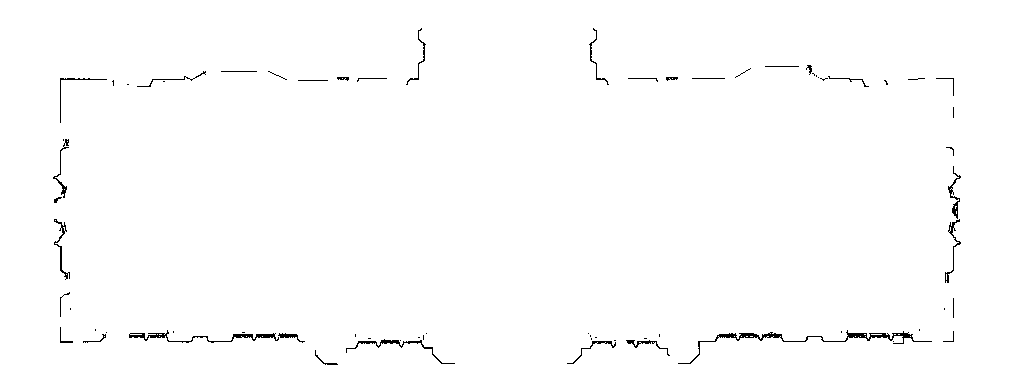
\includegraphics[width=0.7\textwidth]{failed_case.png}} \\
(a) \\
\fbox{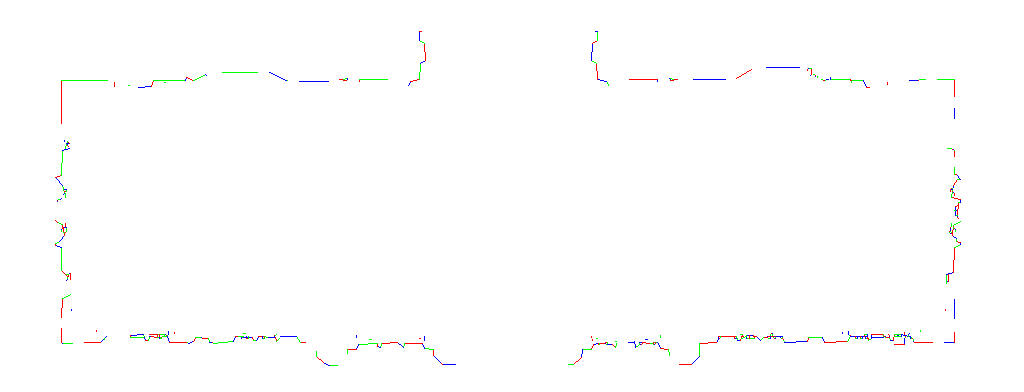
\includegraphics[width=0.7\textwidth]{failed_case_ply.png}} \\
(b) \\
\fbox{\includegraphics[width=0.7\textwidth]{failed_case_bpa.png}} \\
(c)
\end{tabular}
\end{center}
\caption{Binary image vectorization: (a) the example of binary image;
(b) the vectorization result based on DP algorithm;
(c) the vectorization result from proposed BPA algorithm.}
\label{fig:failed_case}
\end{figure*}

The Douglas-Peucker (DP) algorithm \cite{DP_DP} is widely used
to compute boundary vectorization for binary images.
Although the complexity of this approach is $O(nlogn)$ after
the improvement of implementation described in \cite{DP_HS, DP_HS94},
this method cannot fill the holes of the noisy data or
handle the case where spurious interior points are presented.
Agarwal {\it et al.} considered the problem of approximating
a polygon chain using another one to minimize the number of vertices \cite{DP_AV}.
However, for a raster image, the vertices
defining the contour were not known.
For example, \Figa{failed_case} shows a binary cross-section
image of a 3D point cloud data of a building.
\Figb{failed_case} shows the contour generated from DP algorithm.
The problem is that there are
a lot of holes along the contour and the noise inside of the
boundary are modeled inappropriately.
 Medeiros {\it et al.} \cite{BPA_MVL} applied
ball-pivot algorithm (BPA) \cite{BPA_BMRS},
which was original proposed on 3D point cloud data,
on the 2D image to obtain vectorized contour.
The 2D BPA algorithm works well and efficiently on
computing contours with appropriate parameters.
The key parameter for BPA to work successfully is
the size of the ball for pivoting.
We have proposed an adaptive BPA algorithm to address this problem.
\Figc{failed_case} shows
the contour computed by the proposed method which fills holes between gaps
and suppresses noise inside the boundary.


\begin{figure*}[hbtp]
\begin{center}
\begin{tabular}{c}
\includegraphics[width=0.6\textwidth]{BPA_init.pdf} \\
(a) \\
\includegraphics[width=0.6\textwidth]{BPA_refine.pdf} \\
(b)
\end{tabular}
\end{center}
\caption{Adaptive ball pivoting algorithm:
(a) initial pivoting with a ball of radius 2$r$;
(b) refinement with a ball of radius $r$.}
\label{fig:BPA}
\end{figure*}


The original Ball Pivot Algorithm (BPA) was proposed to efficiently
generate 3D mesh representation on 3D point cloud data.
The idea of the BPA is straight-forward:
pivot a ball on a starting point in the image
until it touches another data point as depicted in \Figa{BPA}.
Add the new touched
data point into an ordered list as the vertices of the contour polygon and
set it as the new pivoting point.
Keep doing this pivoting process until all data points are touched.

\section{Boundary Vectorization}

The basic idea behind the proposed framework
for contour computation is as follows:
apply BPA on a selected starting point until
either the ball pivots back to the starting point
which indicates a closed boundary is detected,
or the ball reaches a gap which means this contour is a non-closed
contour and one of the end points is reached.
Because the ball can start pivoting along either clock-wise direction
or counter clock-wise direction,
another pivoting process at start pivoting from
the alternative direction is conducted.
When both directions have been explored,
a contour computation is done.
After this, a {\it refinement} process is carried out
for each line segments using the same BPA algorithm.
For this refinement, the starting point is now
the first end point of a line
and the stopping case is that the ball reaches the other point
or it reaches a gap as depicted in \Figb{BPA}.

\begin{figure}[htbp]
\begin{center}
\begin{tabular}{cc}
\fbox{\includegraphics[width=0.45\textwidth]{global_init_refine_with_rad_128.png}} &
\fbox{\includegraphics[width=0.45\textwidth]{global_init_refine_with_rad_32.png}} \\
(a) & (b) \\
\fbox{\includegraphics[width=0.45\textwidth]{global_init_refine_with_rad_8.png}} &
\fbox{\includegraphics[width=0.45\textwidth]{global_init_refine_with_rad_1.png}} \\
(c) & (d)
\end{tabular}
\end{center}
\caption{Boundary vectorization of a binary image with (a) radius = 128
(b) radius = 32 (c) radius = 8 (d) radius = 2.}
\label{fig:BPA_refinement}
\end{figure}

Here is more detailed description for the algorithm.
At the initial BPA stage, a relatively large radius $r$ is chosen
as a coarse step to cover all gaps between data points.
The output of the initial BPA, $\boldsymbol{\Phi}$,
contains an ordered list of the boundary data points $\boldsymbol{P}$
and their corresponding directions $\overrightarrow{\boldsymbol{R}}$
in which the ball $C$ starts pivoting.
The BPA refinement process applies a smaller radius, say $r' = r/2$,
to $\boldsymbol{\Phi}$ to get more accurate results, as shown in \Figb{BPA}.
For this stage, the length of each line segment formed by adjacent points is checked,
$\ell = \overline{P_0P_1}$, in $\boldsymbol{\Phi}$.
For long line segments, the BPA is applied between the two adjacent points.
When the ball reaches the second end point,
a new list of ordered boundary points,
$\boldsymbol{\Phi'}$, is inserted into $\boldsymbol{\Phi}$ between $P_0$ and $P_1$.
This process continues until it finishes
checking every adjacent point in $\boldsymbol{\Phi}$.
The refinement algorithm is an iterative process,
and the radius of the pivot ball is reduced for each new iteration.
It stops when $r'$ falls below a threshold $\tau_r$.

The key parameter for the BPA algorithm to work successfully is
to find a good initial size of the ball for pivoting.
Here are some general guidances for choosing the radius.
If a contour is known to be a closed polygon,
the initial radius should be big, e.g. the width of an image,
to cover all gaps along the boundary.
Otherwise, if a boundary consists of sub-boundaries,
one could select a relative small radius to start.

An example on the proposed framework
is shown in \Fig{BPA_refinement}.
The initial BPA takes radius $\tau_r$ = 128,
which produced a coarse contour as shown in \Figa{BPA_refinement}.
\Figb{BPA_refinement} - \Figd{BPA_refinement} show that
the contour is becoming more accurate
as the radius $\tau_r$ decreases from 32 to 2.
Note that the original image size is 1024x392 pixels
as shown in \Figa{failed_case}.

\section{Contour Simplification}
\label{sec:BPA_HT}
%%% Adaptive BPA + HT %%%%

Although the proposed framework is an efficient and straightforward
approach to vectorize the contours of noisy images,
it produces many short line segments which can be merged.
In particular, when the underlying boundary is a straight line structure,
the BPA produces excessive un-necessary short lines due to its way
of generating the contour.
An example is shown in the upper part of the contour in \Figb{HT_BPA_figure}
where each colored segment represents a contour edge.
One way to reduce the number of vertices of the polygon is to apply
the approximation polygon method in \cite{DP_AV}.
The drawback of this method is that the topological structures,
such as straight lines, would be lost.
To solve this issue, an adaptive Hough transform (AHT) based method is proposed to replace
short line segments with long lines and potentially eliminate noisy
or outlier vertices around the boundary.
The pseudo-code of the adaptive Hough transform is shown in Algorithm \ref{alg.AHT}.

To combine the adaptive BPA with AHT,
we have to apply AHT on binary images to obtain straight lines.
The straightforward choice for the input binary image
is the original sliced raster image.
However, the issue is that some spurious lines may be detected
because of noise or non-boundary data points,
such as those inside the contour of the raster image
as shown in \Figa{HT_BPA_figure}.
Therefore, a better choice is to use the binary image
generated using the line segments from BPA.
This will solve the spurious line issue because there is only
boundary data points associated with these line segments.
These {\it clear} images can be generated by drawing lines
on blank images using the information of these line segments.

The next step is to apply the HT algorithm on the clear image $I$
to obtain all straight lines $\boldsymbol{L}$ and sort them by length.
The longer lines give higher confidence
to the line structure of the underlying images.
Then a dilation operation \cite {book_gw}
with 8-connected neighbors on $I$
can be used to get the dilation image, $I_d$.
The details on mathematical morphology are
elaborated in Appendix \ref{apdx:mm} for self-containing purpose.
We can measure how well the lines in $\boldsymbol{L}$ match with
the data points in $I_d$,
which determines whether a line in $\boldsymbol{L}$
should be used as a substitution or not.

\begin{figure*}[htbp]
\begin{center}
\begin{tabular}{c}
\fbox{\includegraphics[width=0.7\textwidth]
{aaa_image_slice_0529.png}} \\
(a) \\
\fbox{\includegraphics[width=0.7\textwidth]
{bbb_image_slice_1024_392_0533_refine_with_rad_1_and_merged.png}} \\
(b) \\
\fbox{\includegraphics[width=0.7\textwidth]
{bbb_image_slice_1024_392_0533_combine_HT_BPA_rad_32.png}} \\
(c)
\end{tabular}
\end{center}
\caption{Boundary vectorization of noisy binary image:
(a) the binary image to be processed;
(b) the contour computed by proposed method;
(c) the contour obtained by simplification with Hough transform.}
\label{fig:HT_BPA_figure}
\end{figure*}

If a line segment $L$ is found to be a good candidate,
the corresponding part of the BPA points in $\boldsymbol{\Phi}$
is to be located for substitution.
This is done by first computing the closest two points
$P_i$ and $P_j$ in $\boldsymbol{\Phi}$ to the two end points of $L$.
If the vertices in $\boldsymbol{\Phi}$ represent a polygon,
they will have a closed region layout,
i.e., $\boldsymbol{P} = \{ P_0,P_1,\ldots ,P_{n-1}, P_0 \}$.
Assuming $i < j$, there are two possible choices to replace
the series of the points:
$\boldsymbol{P_1} = \{ P_i,P_{i+1},\ldots,P_{j-1}, P_j \}$, or
$\boldsymbol{P_2} = \{ P_j,P_{j+1},\ldots,P_{i-1}, P_i \}$.
To determine which choice is an appropriate one,
one can compare the distance, $D$,
from the line $L$ to both set of the points
$\boldsymbol{P_1}$ and $\boldsymbol{P_2}$.
The point set with smaller $D$ is the one to be substituted by the line $L$.
\begin{equation*}
D = \underset{\boldsymbol{P_1},\boldsymbol{P_2}}{\operatorname{arg\,min}}
\sum{\lVert P_i - L \rVert}
\qquad P_i \in \boldsymbol{P_1} \ \text{or} \ P_i \in \boldsymbol{P_2}
\end{equation*}
where $\lVert P_i - L \rVert$ is the Euclidean distance
from point $P_i$ to line $L$.

After the integration of BPA contour with the Hough transform lines,
the beautified contour is shown in \Figc{HT_BPA_figure}.
Notice that the top part of the contour,
which consists of short line segments,
was replaced with two long line segments.
As one can see, this process reduces the noise,
simplifies the contour,
and produces clean results
for contours with straight line structures.

\begin{figure}[htbp]
\begin{center}
\begin{tabular}{ccc}
\fbox{\includegraphics[width=0.3\textwidth]{image_slice_0954.png}} &
\fbox{\includegraphics[width=0.3\textwidth]{image_slice_0954_ply.png}} &
\fbox{\includegraphics[width=0.3\textwidth]{image_slice_0954_rad_4_and_merged.png}} \\
(a) & (b) & (c) \\
\fbox{\includegraphics[width=0.3\textwidth]{image_slice_0491_p1.png}} &
\fbox{\includegraphics[width=0.3\textwidth]{image_slice_0491_p1_ply.png}} &
\fbox{\includegraphics[width=0.3\textwidth]{image_slice_0491_p1_rad_4_and_merged.png}} \\
(d) & (e) & (f) \\
\fbox{\includegraphics[width=0.3\textwidth]{image_slice_0341.png}} &
\fbox{\includegraphics[width=0.3\textwidth]{image_slice_0341_ply.png}} &
\fbox{\includegraphics[width=0.3\textwidth]{image_slice_0341_rad_4_and_merged.png}} \\
(g) & (h) & (i) \\
\end{tabular}
\end{center}
\caption{
More experimental results: (a), (d) and (g) show the original noisy binary images;
(b), (e) and (h) show the vectorization results from DP algorithm;
(c), (f) and (i) show the vectorization results from proposed algorithm.}
\label{fig:results}
\end{figure}

In addition to the results shown
in \Fig{failed_case} and \Fig{HT_BPA_figure},
more experimental results are shown in \Fig{results}.
In the first row of \Fig{results},
the input image is of size 1024x392 and contains multiple contours.
In the second row, the input image is 800x640 and contains nested contours.
In the third row, the input image is 800x640 and contains a curved contour.
As demonstrated, the proposed framework can handle all the cases properly
and fill the holes as expected,
which outperformed the standard DP algorithm.


\section{Algorithm Analysis of Boundary Vectorization }

\subsection{Algorithm Analysis of Adaptive Hough Transform }

The Adaptive Hough Transform (AHT) algorithm stems from
the standard Hough transform algorithm.
The function {\it HT()} is a regular Hough Transform (HT),
which returns the lines detected on the image.
The computation complexity of HT is
$O(n^{m-1})$, where $n$ is the size of 2D image
and $m$ is the number of parameters \cite{Hough}.
%http://en.wikipedia.org/wiki/Hough_transform#Limitations
In case of 2D line detection, $m = 2$, and therefore
the complexity is $O(n)$.
The computation of the number of points covered by
each line  ($\rho, \theta$) detected by {\it HT()} is of $O(n)$ complexity.
The image update function {\it update()}
remove data points around the longest line
detected in each iteration, which is of $O(n)$ complexity.
Because we are dealing with bounded number of data points,
and the data points on the longest line of each iteration are removed for each iteration,
the AHT will quickly converge.

\begin{algorithm}
\caption{The Adaptive Hough Transform Algorithm}
\label{alg.AHT}
\begin{algorithmic}[1]
\Procedure {AHTA}{$I$, $\boldsymbol{L}$}
\While {$true$}
\State $\bigcup{(\rho, \theta)} \leftarrow HT (I)$
       \Comment{regular hough transform to get a set of lines}
\State $n \leftarrow 0 $
\For {each $(\rho, \theta) \in \bigcup{(\rho, \theta)} $}
     \State $c \leftarrow num(I, \rho, \theta)$
           \Comment{compute \# of points around line ($\rho, \theta$)}
     \If {$n < c$}
         \State $n \leftarrow c$
         \State $\rho_{max} \leftarrow \rho$
         \State $\theta_{max} \leftarrow \theta$
     \EndIf
\EndFor
\If {$n > \epsilon $}   \Comment{ sanity check for the line ($\rho_{max}, \theta_{max}$) }
\State $\boldsymbol{L} \leftarrow (\rho_{max}, \theta_{max})$
\State $update(I, \rho_{max}, \theta_{max})$
\Else
\State $break$
\EndIf
\If {$\omega(I) < \epsilon$} \Comment{ check how many points left }
\State $break$
\EndIf
\EndWhile
\EndProcedure
\end{algorithmic}
\end{algorithm}

The space complexity of AHT algorithm is bounded
by the space complexity of the {\it HT()} algorithm.
Because we are only working on line detection of 2D images,
the space complexity is $O(n_\rho * n_\theta)$,
where $n_\rho$ and $n_\theta$ represents the number of bins
for quantizing the value of $\rho$ and $\theta$ respectively.
For example, for a image of size 300x400, if we quantize the length $\rho$
with one bin for each pixel, the $n_\rho$ would be 500. Also,
if we quantize the the angle with one bin for a degree,
the $n_\theta$ would be 180.
Based on this, the space complexity for this example can be easily obtained.
The precise of the Hough transform algorithm is depend on the quantization
of the parameters $\rho$ and $\theta$.
The more bins are used for quantization,
the more accurate the results will be,
which implies more space are needed for the algorithm.


\subsection{Algorithm Analysis of Ball-Pivot Algorithm }

\begin{algorithm}
\caption{The 2D Adaptive Ball-Pivot Algorithm}
\label{alg.ABPA}
\begin{algorithmic}[1]
\Procedure {ABPA}{$I$, $\boldsymbol{L}$}
\State $L \leftarrow \emptyset$
\State $P, P_0 \leftarrow Seed(I) $ \Comment{compute the {\it seed} point assigned to $P$ and $P_0$}
\State $r \leftarrow W$ \Comment{initialize radius $r$ with a large value $W$}
\While {$true$}  \Comment{initial BPA stage}
   \State $append(L, P)$
   \State $P_i \leftarrow BPA(P, I, r)$ \Comment{regular 2D BPA}
   \If { $P_i = P_0 $ }
      \State $break$ \Comment { complete the initial BPA }
   \EndIf
   \State $P \leftarrow P_i$ \Comment { find a new vertex $P$ for the contour $L$}
\EndWhile

\State $r \leftarrow W'$ \Comment{a smaller radius $W'$ for refinement}
\While {$r > \epsilon$} \Comment {iterative BPA refinement}
   \For { each line $\overline{P_iP_j} \in \boldsymbol{L} $}
      \State $L' \leftarrow \emptyset$
      \State $P \leftarrow P_i$
      \While {$true$}
         \State $append(L', P)$ \Comment{construct a sub contour $L'$}
         \State $P_k \leftarrow BPA(P, I, r)$
	 \If { $P_k = P_j $ } \Comment{stop when reaching the other point}
	    \State $substitute(L, P_i, P_j, L')$ \Comment{refine $\overline{P_iP_j}$ with $L'$}
	    \State $break$
	 \ElsIf { $isGap(L', P_k)$ }  \Comment{stop when reaching a gap}
	    \State $break$
	 \EndIf
	 \State $P \leftarrow P_k$ \Comment { find a new vertex $P$ for $L'$}
      \EndWhile
   \EndFor
   \State $r \leftarrow r/2$  \Comment{reduce the radius for next iteration}
\EndWhile
\EndProcedure
\end{algorithmic}
\end{algorithm}

The 2D adaptive ball-pivot algorithm (ABPA) is summarized in Algorithm \ref{alg.ABPA}.
The seed computation {\it Seed()} is to pick up a good starting point,
which is only $O(1)$ complexity.
The {\it append()} function is to concatenate the control
points, which is only $O(1)$ complexity.
The regular 2D ball-pivot algorithm, {\it BPA()},
carries out the geometry computation on each control point based on the size of the
radius of the ball or circle.
Basically, for each pivoting of the ball, the area
in the image covered by this pivoting is checked.
If there is a data point contained by this area,
the pivoting ends for this control point.
The worst case for computing the whole potential pivoting area is $O(K*n)$,
where $n$ is the total number of pixels on an image $I$
and $K$ is the number of pivoting for each point.
Because the ball is pivoting for a fixed angle, $\delta$,
$K$ is bounded by the value $2\pi/\delta$.
The complexity to pick up the minimum angle of the pivoting is $O(1)$,
therefore, the complexity for the whole 2D {\it BPA()} is $O(n)$.

For the refinement process, each line $\overline{P_iP_j}$ of the boundary generated
in the previous iteration is checked using the same algorithm in {\it BPA()}.
This only takes $O(n)$ complexity.
The {\it substitute()} and {\it isGap()} function insert an extra point
and carry out a simple algebra computation to check whether a gap is encountered.
The complexity for both operations is $O(1)$.
Because the round of the refinement process is bounded by a predefined constant number,
say $C$, the complexity of this refinement is also bounded by $O(C*n) = O(n)$.

The implementation of the ABPA uses $O(n)$ memory space,
where $n$ is the size of the 2D image.
This complexity includes the enqueue/dequeue the control points of the boundary,
the pivoting geometry computation and the {\it substitute()} and {\it isGap()} computations.
Since the user can control the size of slices,
memory requirements can be tailored to the available hardware.

%%%%% New Chapter %%%%%
%%%%% New Chapter %%%%%
\newchapt{Tapered Structure Detection}{chapt_taper}{Tapered Structure Detection}

After the keyslices are detected and vectorized, the contours of
${\bf N_K} = \{I_i | i = 0, ..., K \}$ keyslices are used to represent
the building based on the extrusion operation.
That is, the space between each pair of keyslices, say $I_{i}$ and $I_{j}$,
can be interpolated by the lower keyslice, e.g., $I_{i}$ in this case.
This is valid because of the similarity between the intermediate slices
and the keyslice $I_{i}$.
By modeling a building using this series of keyslices ${\bf N_K}$,
we significantly reduce the number of polygons for urban buildings.
An example of the reconstructed model is shown in \Fig{DXF_notaper_model}.
This helps make possible of 3D web-based applications,
such as 3D city navigation.

\begin{figure}[htbp]
\begin{center}
\begin{tabular}{c}
\includegraphics[width=0.6\textwidth]{notaper_8_4.png}
\end{tabular}
\end{center}
\caption{ The reconstructed model based on extrusion operation on keyslices. }
\label{fig:DXF_notaper_model}
\end{figure}

In addition to the extrusion operation,
we can potentially further improve the model and reduce the model size
based on the observation that part of the keyslice images
belong to the same tapered structure.
\Figa{DXF_top} shows the roof structure of the reconstructed model
from a keyslice image extrusion operation with
almost half of the keyslices dedicated to the tapered structure.
After inferring the tapered structure, \Figb{DXF_top} shows the improvement
of the modeling, which is much smoother than the previous model.
In addition, the keyslices needed to represent the building,
and its associated storage, are reduced in half.

\begin{figure}[htbp]
\begin{center}
\begin{tabular}{c}
\includegraphics[width=0.7\textwidth]{extrude_1.png} \\
(a) \\
\includegraphics[width=0.7\textwidth]{extrude_2.png} \\
(b)
\end{tabular}
\end{center}
\caption{The top view of the 3D building shown (a) without tapered structures
and (b) with tapered structures.}
\label{fig:DXF_top}
\end{figure}

The difficulty in inferring tapered structures is tied to
the complexity of a building structure itself.
Although the majority of building tapered structures are
{\it linear tapering},
such as {\it tapering to point} (TTP), a cone shape geometry,
as illustrated in \Figa{taper_cases},
and {\it tapering to line} (TTL), a wedge shape geometry,
as shown in \Figb{taper_cases},
it could also be a complicated {\it non-linear tapering},
such as a dome shape geometry which is depicted in \Figc{taper_cases}.
Furthermore, a structure may look like a tapered structure,
but it is actually not a real one.
For example, a series of small extruded structures
form a tapering-like shape in \Figd{taper_cases}.

%% linear_TTP: show a structure from a circle?
%% linear_TTL: show a structure from the FRONT top of the building (the only one)
%% nonlinear_taper: show a structure from Siavash
%% nontaper_TTP: show a structure from Miami court.

\begin{figure}[htbp]
\begin{center}
\begin{tabular}{cc}
\includegraphics[width=0.45\textwidth]{tapering_case1.png} &
\includegraphics[width=0.45\textwidth]{tapering_case2.png} \\
(a) & (b) \\
\includegraphics[width=0.45\textwidth]{tapering_case3.png} &
\includegraphics[width=0.45\textwidth]{tapering_case4.png} \\
(c) & (d)
\end{tabular}
\end{center}
\caption{The component of (a) tapering to a point (b) tapering to a line
(c) non-linear tapering (d) non-tapering. }
\label{fig:taper_cases}
\end{figure}

%%%
% INTRODUCTION goes here
%%%
Although modeling of tapered structure on building volumetric data
has not been exploited much,
a more generic topic which is the modeling of deformable primitives
has being an active research area for a long time.
Numerous work have been proposed by researchers on modeling deformation
primitives \cite{TSI_LJS,TSI_ZY,TSI_CJB}.
The candidate set of primitives include geons, superquadrics and
generalized cylinders, etc.
In \cite{TSI_LJS}, Leonardis proposed the ``recover and select''
paradigm, which simultaneously fits
many different models to the data and dynamically selects the most
promising candidates while filtering out those that match the data poorly.
This work deals with the unsegmented data directly and
is time consuming due to possible multiple primitives existing in the dataset.
The capability of dealing with multiple primitives is not necessary
because our input data has been segmented as described in \Sec{mseg}.

Biederman proposed to use geons to
represent cuboids and cylinders,
as well as curved and tapering versions of these base shapes in his
theory of Recognition by Components \cite{TSI_IB}.
Generalized cylinders extend the concept of a cylinder
by allowing the cross-sectional shape to change
as a function of position along the axis \cite{TSI_TB}.
Also superquadrics are proposed to represent
spheres, cylinders, cuboids, octahedrons,
and interpolations between these shapes \cite{TSI_AHB,TSI_AHB2}.
Zhou and Kambhamettu extended the basic superquadrics
to allow more complex shapes that bend or taper \cite{TSI_ZK}.
Essentially, all those models are fit to 3D data by searching for the parameters
that best align the models' surface with the data.
However, the large number of parameters in these representations
and potential for local minima in the optimization function
presents challenges for these data fitting problems.


%%% bring back to our solution
For building modeling, the major tapered structures
are those linear tapering to a line or tapering to a point structures.
Our intention is to rule out non-tapered structures as well as
those complicated non-linear tapered structures which
we do not want to handle for the sake of simplicity and efficiency.
We only want to infer the relative simple tapered structures,
including linear tapering to a point and tapering to a line.
If the underlying structure is one of the above shapes,
its keyslices can be substituted with the representation of these shapes.
Otherwise, we can choose to model this special structure by fitting a
triangular mesh to the underlying 3D point cloud to produce a polygonal model.

\section{Inferring Linear Tapered Structure}
\label{sec:tsd}

We first check whether it is necessary to do tapering detection by
examining the keyslices computed from all major sweeping directions.
If the segment under analysis can be interpreted
by a few keyslices from certain sweeping direction,
we mark this segment as extrusion structure and therefore
skip the tapering detection for it.
Otherwise, the tapering detection
will be conducted in standard bottom-up direction.
For example, \Figa{taper_extrusion_ttl1} shows a snapshot 
of the point cloud data of a special tapering to line structure.
\Fig{taper_extrusion_ttl1} (b) - (d) show
the keyslices computed from the three principle axes
represented in blue, green and red.
This model can be regarded as an extrusion structure since it
can be interpreted by an extrusion operation on a single keyslice
from left-right direction as shown in \Figd{taper_extrusion_ttl1}.
However, the tapering detection has to be conducted on the models shown
in \Fig{taper_extrusion_ttl2}, \Fig{taper_extrusion_ttp}
and \Fig{taper_extrusion_dome} since they are not able to be interpreted
as simple extrusion operation on a few keyslices.

\begin{figure}[htbp]
\begin{center}
\begin{tabular}{cc}
\includegraphics[width=0.45\textwidth]{taper_ttl1_0.png} &
\fbox{\includegraphics[width=0.45\textwidth]{taper_ttl1_1.jpg}} \\
(a) & (b) \\
\fbox{\includegraphics[width=0.45\textwidth]{taper_ttl1_2.jpg}} &
\fbox{\includegraphics[width=0.45\textwidth]{taper_ttl1_3.jpg}} \\
(c) & (d)
\end{tabular}
\end{center}
\caption{The modeling of a special tapering to line structure:
(a) the snapshot of the point cloud data;
(b) keyslices computed from bottom-up direction;
(c) keyslices computed from face-inside direction;
(d) keyslices computed from left-right direction.
}
\label{fig:taper_extrusion_ttl1}
\end{figure}



\begin{figure}[htbp]
\begin{center}
\begin{tabular}{cc}
\includegraphics[width=0.45\textwidth]{taper_ttl2_0.png} &
\fbox{\includegraphics[width=0.45\textwidth]{taper_ttl2_1.jpg}} \\
(a) & (b) \\
\fbox{\includegraphics[width=0.45\textwidth]{taper_ttl2_2.jpg}} &
\fbox{\includegraphics[width=0.45\textwidth]{taper_ttl2_3.jpg}} \\
(c) & (d)
\end{tabular}
\end{center}
\caption{The modeling of a regular tapering to line structure:
(a) the snapshot of the point cloud data;
(b) keyslices computed from bottom-up direction;
(c) keyslices computed from face-inside direction;
(d) keyslices computed from left-right direction.
}
\label{fig:taper_extrusion_ttl2}
\end{figure}

\begin{figure}[htbp]
\begin{center}
\begin{tabular}{cc}
\includegraphics[width=0.45\textwidth]{taper_ttp_0.png} &
\fbox{\includegraphics[width=0.45\textwidth]{taper_ttp_1.jpg}} \\
(a) & (b) \\
\fbox{\includegraphics[width=0.45\textwidth]{taper_ttp_2.jpg}} &
\fbox{\includegraphics[width=0.45\textwidth]{taper_ttp_3.jpg}} \\
(c) & (d)
\end{tabular}
\end{center}
\caption{The modeling of a tapering to point structure:
(a) the snapshot of the point cloud data;
(b) keyslices computed from bottom-up direction;
(c) keyslices computed from face-inside direction;
(d) keyslices computed from left-right direction.
}
\label{fig:taper_extrusion_ttp}
\end{figure}


\begin{figure}[htbp]
\begin{center}
\begin{tabular}{cc}
\includegraphics[width=0.45\textwidth]{taper_dome_0_1.png} &
\fbox{\includegraphics[width=0.45\textwidth]{taper_dome_1.jpg}} \\
(a) & (b) \\
\fbox{\includegraphics[width=0.45\textwidth]{taper_dome_2.jpg}} &
\fbox{\includegraphics[width=0.45\textwidth]{taper_dome_3.jpg}} \\
(c) & (d)
\end{tabular}
\end{center}
\caption{The modeling of a non-linear tapered structure:
(a) the snapshot of the point cloud data;
(b) keyslices computed from bottom-up direction;
(c) keyslices computed from face-inside direction;
(d) keyslices computed from left-right direction.
}
\label{fig:taper_extrusion_dome}
\end{figure}

We proposed a two-step workflow to accomplish the tapering detection.
The first step is to locate the potential tapering keyslices
and infer the structure by making an assumption that
the underlying tapered structure is either a TTP or a TTL.
With this assumption, we check the last keyslice image of the
potential tapered structure and analyze whether the whole structure
is a TTP or a TTL.
Unfortunately, the tapered structure under analyzing may not
belong to these shapes.
Therefore, a verification step is carried out to check the correctness
of the inferred shape by measuring the error between the model and
the corresponding {\it sampled} 3D point cloud data.
By computing only sampled data points, we can largely
reduce the computation requirement for large-scale PCD.
If the average error is small, the inferred shape is confirmed
and the underlying keyslices are substituted.
Otherwise, we can choose to model this special structure
by meshing the underlying 3D point clouds to produce polygonal model
or simply by the tapering keyslices.

The assumption of linear tapering to a line or point makes the
tapered structure inference much simpler and more efficient.
For keyslice set ${\bf N_K} = \{I_i | 0 \le i \le N \}$,
where $i$ is the projected slice index, we first compute
the sets of keyslices for potential tapered structures.
This is based on the observation that for tapered structures,
the underlying keyslices indices form nearly an arithmetic progression.
\Figb{taper_extrusion_ttl2} and \Figb{taper_extrusion_ttp}
depict the underlying keyslices from bottom-up direction
forming a tapering to a line and tapering to a point respectively.
That is, $ {\bf N_T } = \{ I_t | I_t \in {\bf N_K} \}$,
and for any two successive indices, $i,j$,
we have $ c_1 \le | index(I_i) - index(I_j) | \le c_2 $,
where $c_1$ and $c_2$ are two constants.
In practice, $|c_1 - c_2| \le 1$ and the common difference
for the arithmetic progression is either 3 or 4.

The keyslice set ${\bf N_T}$ indicates a potential section of a
tapered structure in the projected range.
${\bf N_T}$ also provides a very important information for inferring the
underlying structure: based on the assumption, the first element, $I_0$,
in ${\bf N_T}$ is the base geometry shape for the linear tapered structure.
And the last element, $I_f$, of ${\bf N_T}$
is the converged or partially converged geometry shape.
If $I_f$ contains either a line segment or a point structure,
this indicates that the underlying tapered structure of ${\bf N_T}$
is completely converged, as illustrated in \Figa{taper_cases} and
\Figb{taper_cases}.
If $I_f$ contains a polygon structure,
the underlying tapering of ${\bf N_T}$ is partially
converged structure, which is also called {\it tapering to offset},
as depicted in \Figa{offset_taper} and \Figb{offset_taper}.

\begin{figure}[htbp]
\begin{center}
\begin{tabular}{cc}
\includegraphics[width=0.45\textwidth]{offset_polygon.png} &
\includegraphics[width=0.45\textwidth]{offset_circle.png} \\
(a) & (b)
\end{tabular}
\end{center}
\caption{ Tapering to offset structures: (a) tapering to offset with a polygon base;
(b) tapering to offset with a circle base }
\label{fig:offset_taper}
\end{figure}

To compute geometry primitives in $I_f$,
we first compute the bounding box
$[X_{min}, X_{max}], [Y_{min}, Y_{max}]$ for $I_f$.
Then, the distance
$ T_d = max ( |X_{min} - X_{max}|, |Y_{min} - Y_{max}| )$ is checked.
If $T_d < \delta$, where $\delta$ is small threshold, say 4 pixels,
we regard the underlying structure $m$ as a linear tapering to a point.
\Figa{taper_end_slice} shows such a geometry primitive.
To represent this TTP structure,
the control points of the vectorized based geometry image
and the centroid of the $I_f$ are used for reconstruction.

If $T_d >= \delta$, we compute all line segments ${\bf L_f}$ in $I_f$
using the adaptive Hough transform described in Algorithm \ref{alg.AHT}.
If ${\bf L_f}$ only contains one line segment $l = (p_1, p_2)$,
as shown in \Figb{taper_end_slice},
the underlying tapering is completely converged to a line.
To represent this TTL structure,
we compute the converging point for each control point $p(x, y)$
of the vectorized contour of $I_0$,
which is given by the smaller distance,
$min(\overline{pp_1}, \overline{pp_2})$.

\begin{figure}[htbp]
\begin{center}
\begin{tabular}{ccc}
\fbox{\includegraphics[width=0.3\textwidth]{taper_end_slice_0.png}} &
\fbox{\includegraphics[width=0.3\textwidth]{taper_end_slice_1.png}} &
\fbox{\includegraphics[width=0.3\textwidth]{taper_end_slice_2.png}} \\
(a) & (b) & (c)
\end{tabular}
\end{center}
\caption{The converged slice $I_f$ for various tapered structures:
(a) tapering to point;
(b) tapering to line;
(c) tapering to offset.
}
\label{fig:taper_end_slice}
\end{figure}

When ${\bf L_f}$ contains multiple line segments,
as shown in \Figc{taper_end_slice},
the underlying tapered structure is a tapering to offset structure.
Under the assumption, the virtually converged shape
could be either a line or a point.
To infer the underlying structure,
we first compute the median length $l_m$ of all line segments in ${\bf L_f}$.
If $l_m$ is larger than the threshold, say $l_m > 10$,
the base geometry shape $I_0$ is usually a regular polygon structure
as shown in \Figa{offset_taper}.
We compute the intersection points of all lines for both $I_f$ and $I_0$.
If the total number of intersection points matches,
we can represent this tapered structure using the control points
in $I_0$ and their corresponding control points in $I_f$.

If $l_m$ is smaller than or equal to the threshold,
the shape of $I_f$ is usually a circle or other curved shapes,
rather than a regular polygon structure as shown in \Figb{offset_taper}.
We regard the underlying structure as a converging to a point structure.
To represent this structure,
we cannot match each control point in $I_0$ with its corresponding
converging point in $I_f$ anymore.
Therefore, we compute the virtual converged point $P_v$
using the triangular equation.
We compute the centroids $P_{c1}$ and $P_{c2}$
and the average distance $d_1$ and $d_2$ from data points to centroids
for both $I_f$ and $I_0$.
$P_v$ can be computed by,
\begin{equation*}
\frac{d_1}{d_2} = \frac{|P_v - P_{c1}|}{|P_v - P_{c2}|}
\end{equation*}
Once $P_v$ is computed, the actual partially converged point $P_x$
for the control point $P$ can be computed as,
\begin{equation*}
\frac{d_1}{d_2} = \frac{|P_v - P_x|}{|P_v - P|}
\end{equation*}

\section{Verification of Inferred Tapered Structure}
\label{sec:vts}

%% step1: compute all the planes formed by the based geometry
%%        and the converged point
%%
%% step2: sampling the data representing the potential section.
%%        sample a data point, check whether it is following into
%%        the section.
%%
%% step3: compute the distance using the equation...

After applying the approach described in \Sec{tsd}, we need to verify
whether the new detected shape is valid or not.
This is because the assumption we made in \Sec{tsd} that
the underlying tapered structure is either TTP or TTL.
This assumption may not be held for some complicated cases
as shown in \Figc{taper_cases} and \Figd{taper_cases}.
The basic idea for the verification stage is to measure the error
for the new inferred tapered structure.
For large-scale PCD, it would be time consuming to compute
the error for all eligible data points.
Therefore, we only sample a certain amount of data points for
error measurement.

Let $N_c$ and $N_t$ be the current number and the total number of
data points for error measurement.
A data point $p(x, y, z)$ from current PCD segment is sampled via
uniform sampling process.
We first compute the 2D sliced index $I_p$ for $p$ using \Eq{image_slicing}.
If $I_0 \le I_p \le I_f$, that is, the point $p$ is between the
height range of the base location and converged location,
$p$ is regarded as a good sampled data and is used for further
error computation, which increases $N_c$ by 1.
Otherwise, $p$ is discarded and another round of sampling is carried out.

To compute the distance between $p$ and the inferred model $M$,
we first compute all the 3D planes formed by points in the base polygon
$I_0$ and the converged points in the $I_f$.
Given two consecutive control points $p1, p2$ in $I_0$, and
the third converged point $p3$ in $I_f$, the plane $P_t$ can be computed using
the equation \Eq{plane_3pts} as described in Appendix \ref{sec:plane}.
We compute all the planes ${\bf P }$ for the tapered structure $M$.

\begin{figure}[htbp]
\begin{center}
\begin{tabular}{c}
\includegraphics[width=0.6\textwidth]{taper_dome_0.png} \\
(a) \\
\includegraphics[width=0.6\textwidth]{taper_dome_4.png} \\
(b)
\end{tabular}
\end{center}
\caption{The verification of the inferred tapered structure:
(a) the original model;
(b) the computed keyslices (in white) and inferred tapering to point structure (in blue).
}
\label{fig:taper_taper_dome}
\end{figure}

The distance between a 3D point $p(x, y, z)$ and a plane $P_t$ is given by
\Eq{dist_pt2pl} as shown in Appendix \ref{sec:plane}.
The distance between $p$ and the structure $M$ is defined as the minimum
distance from $p$ to all planes in ${\bf P }$.
that is, $d_p = min(p, P_t)$, where $P_t \in {\bf P}$.
Therefore, the average error for the tapered structure $M$ is defined as
%$E_M = \frac{\sum_p(d_p)}{N_t} $
$E_M = \sum_p(d_p)/N_t$.
If $E_M$ is smaller than a threshold, $t$,
the tapered structure is approved and
the corresponding keyslices are substituted to further compress the model.
Otherwise, the underlying tapered structure is rejected,
and we can choose to model this special structure by its keyslices or
by fitting a triangular mesh to the underlying 3D point cloud
to produce a polygonal model.
\Fig{taper_taper_dome} shows a dome model which was first modeled
as a taper to a point structure (in blue)
but later on was rejected by the verification process.
We chose $t = \tau_d/2$ as the threshold,
and it worked well on our synthetic and real datasets.
Here, $\tau_d$ is the threshold for keyslice detection
as introduced in \Sec{ksd}.


%%%%% New Chapter %%%%%
%%%%% New Chapter %%%%%
\newchapt{Model Generation}{chapt_gen}{Model Generation}

In previous chapters, we have segmented the original 3D PCD,
computed the keyslices and their contours for each segment,
and identified tapered structures.
All these computation lead to the final stage of model generation.
The reconstruction of a single segment is straightforward:
transform the underlying 2D geometry into 3D coordinate system.
For each segment, we first exam whether it can be modeled
by extrusion operation on simple keyslices along any major plane.
For an extrusion segment, it is a push-pull operation
of the basic geometry along its sweeping direction;
for a tapered segment, the faces formed by the control points
of the base geometry polygon and their corresponding converged points
are constructed.

The results of the extrusion and tapered structures computation,
together with keyslice image vectorization,
are stored in the 2D image coordinate system.
To generate the 3D model, these results need to be transformed
back into the 3D world coordinate system.
Let $P(x,y)$ be a point in the 2D image coordinate system,
and let $P'(x,y,z)$ be the 3D world coordinate of $P$,
where $y$ is the bottom-up (height) coordinate.
For all points in the same contour,
they lie in the same plane and hence share the same value of $y$.
The equation for transforming $P$ back to $P'$ is as follows,
%[\,x^{3D},\; y^{3D},\; z^{3D}\,]^T = [\,\eta\cdot x^{2D} + X_{MIN},\;
%\zeta + Y_{MIN},\; \eta\cdot z^{2D} + Z_{MIN}\,]^T
\begin{equation}
\left(
\begin{array}{c}
x^{3D} \\
y^{3D} \\
z^{3D}
\end{array}
\right) =
\left(
\begin{array}{ccc}
\eta & X_{min} & 0 \\
0 & \zeta + Y_{min} & 0 \\
0 & Z_{min} & \eta
\end{array}
\right)
\left(
\begin{array}{c}
x^{2D} \\
1 \\
z^{2D}
\end{array}
\right)
\label{eq:ir2dxf}
\end{equation}
%Note that $\omega = W/(X_{max} - X_{min})$, and that
where $\eta=(X_{max} - X_{min})/W$,  $\zeta=\kappa\cdot\delta$,
$\kappa$ is the index of the 2D slice
and $\delta$ is the height of a slab.
Note that [$X_{min}$, $X_{max}$], [$Y_{min}$, $Y_{max}$],
and [$Z_{min}$, $Z_{max}$] pairs define the 3D bounding box,
and $W$ is the width of the 2D sliced image
as described in \Sec{image_slicing}.


\section{Model Merging}

Because the whole point clouds of a building
may be partitioned into segments for modeling,
we need to assemble those segments to obtain the final model.
Furthermore, the extrusion operation on 2D keyslice contours
may introduce discrepancy on vertices and edges for the adjacent keyslices.
Therefore, model merging needs to be carried out for
correctly reconstructing the model.
Essentially, this process is to merge the vertices and edges shared by
the adjacent keyslices or neighboring segments.

\begin{figure}[htbp]
  \centering
  \includegraphics
      [width=\textwidth]
      {model_merge.pdf}
      \caption{Vertices adjustment for model merging:
      (a) the two new points $Q_0$ and $Q_1$ are projected to
          an existed line as $Q'_0$ and $Q'_1$;
      (b) after (a), $Q'_1$ is merged with an existed point $P_1$;
      (c) after (a), both $Q'_0$ and $Q'_1$ are merged with
          existed point $P_0$ and $P_1$ respectively;
      (d) one of the point $Q_1$ is too far away for adjustment. }
      \label{fig:MR_Fig1}
\end{figure}

The first segmented part can be easily reconstructed without merging.
Let ${\bf M}$ represent all lines or planes added into the final model so far.
When adding a new line segment $Q_0Q_1$ to the model,
we need to compute the closest line ${\bf L} = P_0P_1$ in ${\bf M}$ to $Q_0Q_1$.
Let $d = max(dist(Q_0, {\bf L}), dist(Q_1, {\bf L}))$, i.e., the larger distance
between $Q_0$ to ${\bf L}$ and $Q_1$ to ${\bf L}$.
The distance from a point $Q$ to a line ${\bf L}$ can be computed using the equation:
\begin{equation*} % point to line equation
d(Q, { \bf L}) = | {\bf w - (w \cdot u) \, u} |
\end{equation*}
where ${\bf w} = (Q - P_0) $ and {\bf u} is the unit direction vector of {\bf L}.

There are several cases to be considered.
If $d <= \delta$, that is, both $Q_0$ and $Q_1$ are close enough to $L$,
the projected point $Q'_0$ and $Q'_1$
are used to replace $Q_0$ and $Q_1$ respectively as shown in \Figa{MR_Fig1}.
Furthermore, if one of the projected point,
say $Q'_1$ is close to an end point of $L$, say $P_1$,
$Q'_1$ would be merged with $P_1$ as shown in \Figb{MR_Fig1}.
If both $Q'_0$ and $Q'_1$ are matched with $P_0$ and $P_1$,
the line $Q_0Q_1$ would be merged totally with the line $L$,
which was shown in \Figc{MR_Fig1}.
However, if $d > \delta$, no merging should be conducted as shown in \Figd{MR_Fig1}.
\Figa{MR_Fig2} and \Figb{MR_Fig2} show the structures before and after
being merged.


\begin{figure} [htbp]
\begin{center}
\begin{tabular}{cc}
\includegraphics[width=0.45\textwidth]{model_before_merge.png} &
\includegraphics[width=0.45\textwidth]{model_after_merge.png} \\
(a) & (b)
\end{tabular}
\end{center}
\caption{ Model merging computation:
      (a) two structures inside red ellipse are separated before merged;
      (b) new structures after merged. }
\label{fig:MR_Fig2}
\end{figure}

\section{Window Installation}

After the model merging, the whole reconstructed model has been generated.
We call this {\it naked} model in that there is no windows or doors
being installed yet as shown in \Figa{WDR_Fig1}.
If the point cloud contains windows or doors,
we need to add them onto the naked model.
The window and door structures have been computed as described in Section \ref{sec:wdd}.
The problem is which face or plane should they be added.

\begin{figure} [htbp]
\begin{center}
\begin{tabular}{cc}
\includegraphics[width=0.45\textwidth]{model_naked.png} &
\includegraphics[width=0.45\textwidth]{model_windows.png} \\
(a) & (b)
\end{tabular}
\end{center}
\caption{ Windows and doors reconstruction:
      (a) the reconstructed naked model;
      (b) the whole model with windows and doors added.}
\label{fig:WDR_Fig1}
\end{figure}

Let {\bf M} be the set of lines from a naked model.
Let $Q_0 = [X_{min}, Z_{min}], Q_1 = [X_{max}, Z_{max}]$
define the bounding box of a window $w$,
i.e., $[Q_0, Q_1]$ is the diagonal points for $w$.
Let $[Y_{min}, Y_{max}]$ be the height range of $w$.
The goal is to find the right face (closest line segment) for $w$ to be added.
For each line segment $L = P_0P_1 $ in ${\bf M}$,
we first compute the projected points $Q'_0, Q'_1$
of $Q_0, Q_1$ on $L$ to check whether they are in between $[P_0, P_1]$.
If not, $L$ is not eligible for adding $w$
since a window could not fall outside of a facade.
Otherwise, the extruded range $L_{min}, L_{max}$ of $L$ is computed.
If $Y_{min} > L_{min}$ and $Y_{max} < L_{max}$,
that is, the window $w$ is totally covered by the
extruded face $F$ which is generated from $L$,
$F$ is a potential face for adding $w$.
The distance $d_p = max(|Q_0Q'_0|, |Q_1Q'_1|)$ is used
to compare with global minimum distance $d_{p\_min}$
which was set to be a large value initially.
If $d_p < d_{p\_min}$, which means a closer face for $w$ is found,
$d_{p\_min}$ is updated to $d_p$ and
the corresponding line $L_{win}$ and its face $F_{win}$
are updated to $L$ and $F$ respectively.

When all lines in ${\bf M}$ are checked,
$F_{win}$ will give us the right face for adding $w$.
To add $w$ on $F_{win}$, we need to compute the projected point $P'$
for each vertex $P$ in $w$ on $F_{win}$.
Let $F_{win} = ax + by + cz + d$, the equation to compute $P(x_0, y_0, z_0)$ is
\begin{equation*} % projection point on a plane
P' = P - \frac{(ax_0+by_0+cz_0+d)}{a^2+b^2+c^2}\,{\bf n}
\end{equation*}
where {\bf n} is the normal of $F_{win}$.
This will generate a closed face $F_w$ on $F_{win}$.
A simple push-pull operation on $F_w$ with the distance $d_w$
which was computed in the Section \ref{sec:wdd}
will add the window $w$ onto $F_w$ of the naked model.
\Figb{WDR_Fig1} shows the entire model
with windows and doors added for the model in \Figa{WDR_Fig1}.


\section{Experimental Results}

We have applied the proposed method on both synthetic
and real datasets.
\Fig{ER_Fig1} through \Fig{ER_Fig10} shows the experimental results
for synthetic datasets.
The reconstructed model on real datasets are shown in \Fig{TH_Fig}
through \Fig{GCT_Fig} which are corresponding to
Thomas Hunter building at Hunter College,
Cooper Union building in downtown New York, and
Grand Central Terminal building in middletown New York, respectively.

For each set of the figures, the snapshot of
the original SketchUp model (or the building photo for real dataset),
the point cloud dataset,
the segmentation,
the keyslices,
the extruded model,
and the final models from different viewpoints are shown in order.
If applicable, the snapshot of the tapered model and
the model with windows and doors installed are also shown.
The thresholds used for the computation are $\tau_r = 4$ and $\tau_d = 4$.

% real dataset results

In addition to exterior models,
we have also applied the lightweight
reconstruction algorithm to the range data of interior scans.
The snapshot of an interior scan of Hunter Theater is shown in \Figa{IN}
and its reconstructed 3D model is shown in \Figb{IN}.
This model is primarily reconstructed using the extrusion operation
upon the main structures of the interior.
The chairs and some other fine details were not able to be handled
and therefore were manually culled.
%Please note that the model generated in \Figb{IN} is of low resolution.
%Any lost detail may be recaptured by using a smaller threshold $\tau_d$
%to obtain higher resolution models.

%%%% figures start here
%%%% x_5':  the major facade detection image
%%%% x_6:   the sliced images ??? arrange ???
%%%% x_7':  the model segmentation image
%%%% x_8':  the window/door images if have
%%%% x_9:   the keyslices and BPA images
%%%% x_10': the naked model without windows/doors
%%%% x_11': the extrued only model?

\begin{figure} [htbp]
\begin{center}
\begin{tabular}{ccc}
\includegraphics[width=0.3\textwidth]{cu_1.png} &
\includegraphics[width=0.3\textwidth]{cu_2.png} &
\includegraphics[width=0.3\textwidth]{cu_7.png} \\
(a) & (b) & (c)\\
%\fbox{\includegraphics[width=0.3\textwidth]{cu_8.png}} &
\includegraphics[width=0.3\textwidth]{cu_9.png} &
\includegraphics[width=0.3\textwidth]{cu_11.png} &
\includegraphics[width=0.3\textwidth]{cu_10.png} \\
(d) & (e) & (f)\\
\includegraphics[width=0.3\textwidth]{cu_3.png} &
\includegraphics[width=0.3\textwidth]{cu_4.png} \\
(g) & (h)
\end{tabular}
\end{center}
\caption{ Experimental results of Cooper Union model: the snapshots of
      (a) the original SketchUp model;
      (b) synthetic point cloud data generated from (a);
      (c) segmentation;
      (d) keyslices;
      (e) extruded model;
      (f) tapered model;
      (g) reconstructed model with windows installed (I) ;
      (h) reconstructed model with windows installed (II) .
}
\label{fig:ER_Fig1}
\end{figure}

\begin{figure} [htbp]
\begin{center}
\begin{tabular}{ccc}
\includegraphics[width=0.3\textwidth]{spitak_1.png} &
\includegraphics[width=0.3\textwidth]{spitak_2.png} &
\includegraphics[width=0.3\textwidth]{spitak_7.png} \\
(a) & (b) & (c) \\
%\fbox{\includegraphics[width=0.3\textwidth]{spitak_6.png}} &
\includegraphics[width=0.3\textwidth]{spitak_9.png} &
\includegraphics[width=0.3\textwidth]{spitak_11.png} &
\includegraphics[width=0.3\textwidth]{spitak_3.png} \\
(d) & (e) & (f) \\
\includegraphics[width=0.3\textwidth]{spitak_4.png} \\
(g)
\end{tabular}
\end{center}
\caption{ Experimental results of Spitak model: the snapshots of
      (a) the original SketchUp model;
      (b) synthetic point cloud data generated from (a);
      (c) segmentation;
      (d) keyslices;
      (e) extruded model;
      (f) tapered model;
      (g) reconstructed model.
}
\label{fig:ER_Fig2}
\end{figure}

\begin{figure} [htbp]
\begin{center}
\begin{tabular}{ccc}
\includegraphics[width=0.3\textwidth]{house_1.png} &
\includegraphics[width=0.3\textwidth]{house_2.png} &
\includegraphics[width=0.3\textwidth]{house_7.png} \\
(a) & (b) & (c)\\
\includegraphics[width=0.3\textwidth]{house_9.png} &
\includegraphics[width=0.3\textwidth]{house_11.png} &
\includegraphics[width=0.3\textwidth]{house_3.png} \\
(d) & (e) & (f) \\
\includegraphics[width=0.3\textwidth]{house_4.png} \\
(g)
\end{tabular}
\end{center}
\caption{ Experimental results of apartment model: the snapshots of
      (a) the original SketchUp model;
      (b) synthetic point cloud data generated from (a);
      (c) segmentation;
      (d) keyslices;
      (e) extruded model;
      (f) the model with windows installed;
      (g) reconstructed model.
}
\label{fig:ER_Fig3}
\end{figure}

\begin{figure} [htbp]
\begin{center}
\begin{tabular}{ccc}
\includegraphics[width=0.3\textwidth]{branch_lib_1.png} &
\includegraphics[width=0.3\textwidth]{branch_lib_2.png} &
\includegraphics[width=0.3\textwidth]{branch_lib_7.png} \\
(a) & (b) & (c) \\
\includegraphics[width=0.3\textwidth]{branch_lib_9.png} &
\includegraphics[width=0.3\textwidth]{branch_lib_11.png} &
\includegraphics[width=0.3\textwidth]{branch_lib_3.png} \\
(d) & (e) & (f) \\
\includegraphics[width=0.3\textwidth]{branch_lib_4.png} \\
(g)
\end{tabular}
\end{center}
\caption{ Experimental results of Branch library model: the snapshots of
      (a) the original SketchUp model;
      (b) synthetic point cloud data generated from (a);
      (c) segmentation;
      (d) keyslices;
      (e) extruded model;
      (f) tapered model;
      (g) reconstructed model.
}
\label{fig:ER_Fig4}
\end{figure}

\begin{figure} [htbp]
\begin{center}
\begin{tabular}{ccc}
\includegraphics[width=0.3\textwidth]{clements_lib_1.png} &
\includegraphics[width=0.3\textwidth]{clements_lib_2.png} &
\includegraphics[width=0.3\textwidth]{clements_lib_7.png} \\
(a) & (b) & (c)\\
\includegraphics[width=0.3\textwidth]{clements_lib_9.png} &
\includegraphics[width=0.3\textwidth]{clements_lib_3.png} &
\includegraphics[width=0.3\textwidth]{clements_lib_4.png} \\
(d) & (e) & (f)
\end{tabular}
\end{center}
\caption{ Experimental results of Clements library model: the snapshots of
      (a) the original SketchUp model;
      (b) synthetic point cloud data generated from (a);
      (c) segmentation;
      (d) keyslices;
      (e) extruded model;
      (f) reconstructed model.
}
\label{fig:ER_Fig5}
\end{figure}

\begin{figure} [htbp]
\begin{center}
\begin{tabular}{ccc}
\includegraphics[width=0.3\textwidth]{doe_1.png} &
\includegraphics[width=0.3\textwidth]{doe_2.png} &
\includegraphics[width=0.3\textwidth]{doe_7.png} \\
(a) & (b) & (c) \\
\includegraphics[width=0.3\textwidth]{doe_9.png} &
\includegraphics[width=0.3\textwidth]{doe_11.png} &
\includegraphics[width=0.3\textwidth]{doe_3.png} \\
(d) & (e) & (f) \\
\includegraphics[width=0.3\textwidth]{doe_4.png} \\
(g)
\end{tabular}
\end{center}
\caption{ Experimental results of Doe library model: the snapshots of
      (a) the original SketchUp model;
      (b) synthetic point cloud data generated from (a);
      (c) segmentation;
      (d) keyslices;
      (e) extruded model;
      (f) tapered model;
      (g) reconstructed model.
}
\label{fig:ER_Fig6}
\end{figure}

\begin{figure} [htbp]
\begin{center}
\begin{tabular}{ccc}
\includegraphics[width=0.3\textwidth]{health_town_1.png} &
\includegraphics[width=0.3\textwidth]{health_town_2.png} &
\includegraphics[width=0.3\textwidth]{health_town_7.png} \\
(a) & (b) & (c) \\
\includegraphics[width=0.3\textwidth]{health_town_9.png} &
\includegraphics[width=0.3\textwidth]{health_town_11.png} &
\includegraphics[width=0.3\textwidth]{health_town_3.png} \\
(d) & (e) & (f) \\
\includegraphics[width=0.3\textwidth]{health_town_4.png} \\
(g)
\end{tabular}
\end{center}
\caption{ Experimental results of Health town library model: the snapshots of
      (a) the original SketchUp model;
      (b) synthetic point cloud data generated from (a);
      (c) segmentation;
      (d) keyslices;
      (e) extruded model;
      (f) tapered model;
      (g) reconstructed model.
}
\label{fig:ER_Fig7}
\end{figure}

\begin{figure} [htbp]
\begin{center}
\begin{tabular}{ccc}
\includegraphics[width=0.3\textwidth]{miami_1.png} &
\includegraphics[width=0.3\textwidth]{miami_2.png} &
\includegraphics[width=0.3\textwidth]{miami_7.png} \\
(a) & (b) & (c)\\
\includegraphics[width=0.3\textwidth]{miami_9.png} &
\includegraphics[width=0.3\textwidth]{miami_3.png} &
\includegraphics[width=0.3\textwidth]{miami_4.png} \\
(d) & (e) & (f)
\end{tabular}
\end{center}
\caption{ Experimental results of Miami Date Courthouse model: the snapshots of
      (a) the original SketchUp model;
      (b) synthetic point cloud data generated from (a);
      (c) segmentation;
      (d) keyslices;
      (e) extruded model;
      (f) reconstructed model.
}
\label{fig:ER_Fig8}
\end{figure}

\begin{figure} [htbp]
\begin{center}
\begin{tabular}{ccc}
\includegraphics[width=0.3\textwidth]{simple_1.png} &
\includegraphics[width=0.3\textwidth]{simple_2.png} &
\includegraphics[width=0.3\textwidth]{simple_7.png} \\
(a) & (b) & (c)\\
\includegraphics[width=0.3\textwidth]{simple_9.png} &
\includegraphics[width=0.3\textwidth]{simple_3.png} &
\includegraphics[width=0.3\textwidth]{simple_4.png} \\
(d) & (e) & (f)
\end{tabular}
\end{center}
\caption{ Experimental results of a simple model: the snapshots of
      (a) the original SketchUp model;
      (b) synthetic point cloud data generated from (a);
      (c) segmentation;
      (d) keyslices;
      (e) extruded model;
      (f) reconstructed model.
}
\label{fig:ER_Fig9}
\end{figure}

\begin{figure} [htbp]
\begin{center}
\begin{tabular}{ccc}
\includegraphics[width=0.3\textwidth]{michael_1.png} &
\includegraphics[width=0.3\textwidth]{michael_2.png} &
\includegraphics[width=0.3\textwidth]{michael_7.png} \\
(a) & (b) & (c) \\
\includegraphics[width=0.3\textwidth]{michael_9.png} &
\includegraphics[width=0.3\textwidth]{michael_11.png} &
\includegraphics[width=0.3\textwidth]{michael_3.png} \\
(d) & (e) & (f) \\
\includegraphics[width=0.3\textwidth]{michael_4.png} \\
(g)
\end{tabular}
\end{center}
\caption{ Experimental results of St. Michael church model: the snapshots of
      (a) the original SketchUp model;
      (b) synthetic point cloud data generated from (a);
      (c) segmentation;
      (d) keyslices;
      (e) extruded model;
      (f) tapered model;
      (g) reconstructed model.
}
\label{fig:ER_Fig10}
\end{figure}


%%%% figures start here
%%%% x_5':  the major facade detection image
%%%% x_6:   the sliced images ??? arrange ???
%%%% x_7':  the model segmentation image
%%%% x_8':  the window/door images if have
%%%% x_9:   the keyslices and BPA images
%%%% x_10': the naked model without windows/doors
%%%% x_11': the extrued only model?

\begin{figure} [htbp]
\begin{center}
\begin{tabular}{ccc}
\includegraphics[width=0.3\textwidth]{TH_1.jpg} &
\includegraphics[width=0.3\textwidth]{point_cloud.png} &
\includegraphics[width=0.3\textwidth]{TH_7.png} \\
(a) & (b) & (c)\\
\includegraphics[width=0.3\textwidth]{TH_9.png} &
\includegraphics[width=0.3\textwidth]{TH_10.png} &
\includegraphics[width=0.3\textwidth]{TH_3.png} \\
(d) & (e) & (f)\\
\includegraphics[width=0.3\textwidth]{TH_4.png} \\
(g)
\end{tabular}
\end{center}
\caption{ Experimental results of Thomas Hunter building: the snapshots of
      (a) real building;
      (b) point cloud dataset acquired from laser scanner;
      (c) segmentation;
      (d) keyslices;
      (e) extruded model;
      (f) reconstructed model with windows installed;
      (g) reconstructed model.
}
\label{fig:TH_Fig}
\end{figure}

\begin{figure} [htbp]
\begin{center}
\begin{tabular}{ccc}
\includegraphics[width=0.3\textwidth]{real_cu_1.jpg} &
\includegraphics[width=0.3\textwidth]{real_cu_2.png} &
\includegraphics[width=0.3\textwidth]{real_cu_7.png} \\
(a) & (b) & (c)\\
\includegraphics[width=0.3\textwidth]{real_cu_9.png} &
\includegraphics[width=0.3\textwidth]{real_cu_10.png} &
\includegraphics[width=0.3\textwidth]{real_cu_3.png} \\
(d) & (e) & (f)\\
\includegraphics[width=0.3\textwidth]{real_cu_4.png} \\
(g)
\end{tabular}
\end{center}
\caption{ Experimental results of Cooper Union building: the snapshots of
      (a) real building;
      (b) point cloud dataset acquired from laser scanner;
      (c) segmentation;
      (d) keyslices;
      (e) extruded model;
      (f) reconstructed model with windows installed;
      (g) reconstructed model.
}
\label{fig:real_cu_Fig}
\end{figure}


\begin{figure} [htbp]
\begin{center}
\begin{tabular}{ccc}
\includegraphics[width=0.3\textwidth]{GCT_1.jpg} &
\includegraphics[width=0.3\textwidth]{GCT_2.png} &
\includegraphics[width=0.3\textwidth]{GCT_7.png} \\
(a) & (b) & (c)\\
\includegraphics[width=0.3\textwidth]{GCT_9.png} &
\includegraphics[width=0.3\textwidth]{GCT_10.png} &
\includegraphics[width=0.3\textwidth]{GCT_3.png} \\
(d) & (e) & (f)\\
\includegraphics[width=0.3\textwidth]{GCT_4.png} \\
(g)
\end{tabular}
\end{center}
\caption{ Experimental results of Grand Central Terminal building: the snapshots of
      (a) real building;
      (b) point cloud dataset acquired from laser scanner;
      (c) segmentation;
      (d) keyslices;
      (e) extruded model;
      (f) reconstructed model with windows installed;
      (g) reconstructed model.
}
\label{fig:GCT_Fig}
\end{figure}

%% \begin{figure*}[htbp]
%% \begin{center}
%% \begin{tabular}{c}
%% \includegraphics[width=0.8\textwidth]{HunterShaded.jpg} \\
%% (a) \\
%% \includegraphics[width=0.8\textwidth]{HunterGE.jpg} \\
%% (b)
%% \end{tabular}
%% \end{center}
%% \caption{ (a) rendering of lightweight reconstructed model.
%% (b) The placement of the 3D model on Google Earth.}
%% \label{fig:OUT}
%% \end{figure*}

\begin{figure*}[htbp]
\begin{center}
\begin{tabular}{c}
\includegraphics[width=0.6\textwidth]{range_crop.png} \\
(a) \\
\includegraphics[width=0.6\textwidth]{HunterTheatreShaded.jpg} \\
(b)
\end{tabular}
\end{center}
\caption{The model of an interior scan: (a) the input point cloud data;
(b) the reconstructed lightweight 3D model.}
\label{fig:IN}
\end{figure*}

%%%% figures end here

%%%%% New Chapter %%%%%
%%%%% New Chapter %%%%%
\newchapt{Performance Evaluation}{chapt8}{Performance Evaluation}

\section{Complexity Analysis}
Given a 3D point cloud dataset with $N$ points,
the $k$d-tree construction in the major plane detection
takes $O(NlogN)$ time for both space and computational complexity \cite{NE_KD}.
The query operation for $k$d-tree takes $O(N^{1-1/k})$ time,
where $k$ is the dimension of the $k$d-tree.
The MLS based normal computation is bounded by $O(m)$,
where $m$ is the number of neighbor points.
Because $m$ is bounded by a constant value,
the computational complexity for the major plane detection
is of $O(m*NlogN) = O(NlogN)$.
The space complexity of the whole major plane detection
is also bounded by $O(NlogN)$.

Based on \Eq{image_slicing}, the projection computation for each 3D point
takes only $O(1)$ run time.
Therefore, the projection of 3D point cloud to 2D images algorithm
is of $O(N)$ computational complexity for each major plane.
Because there are only limited number of major planes for a building,
the whole 3D projection process is of $O(N)$ computational complexity.
For our fast projection implementation,
every 3D point is stored in memory and therefore
space complexity of projection is also $O(N)$.

The image processing based algorithms are much cheaper
compared to the above 3D computations.
The noise removal process takes $O(n)$ complexity,
where $n$ is the size of the 2D image.
The hole filling is based on symmetry computation of translation,
which is bounded by $O((w+h)*n)$,
where $w$ and $h$ are the width and height of the 2D image.
Therefore, the complexity of the hole filling is $O(n)$.

As pointed out in \Sec{aa_kd}, the keyslice detection algorithm
takes $O(n)$ complexity.
The boundary vectorization algorithm also takes $O(n)$ complexity.
The space complexity of both the keyslice detection and
the boundary vectorization is also bounded by $O(n)$.
The tapering detection algorithm consists of two stages.
The first stage is based on the keyslices computed earlier,
and is bounded by the complexity of $O(n)$.
The second stage which computes the errors
for the reconstructed tapered model is bounded by $O(N)$.
As we know, $N > n$, therefore the overall time and space complexity
for the whole system is bounded by $O(NlogN)$.


\section{Parameters and Error Estimation}
\label{sec:pf_ee}

To measure the error of a reconstructed 3D model,
we first transform it to the 3D point cloud coordinate system.
The error $E$ is measured as the distance
between the 3D points in the point cloud dataset
and their closest planes in the reconstructed model $M$:
\begin{equation}
E = \frac{1}{|X|}\sum_{x\in{X}}{d(x, M)}
\label{eq:em}
\end{equation}
where $X$ is the set of 3D points in the point cloud,
and distance $d(x, M) = \text{min}_{p \in M}\lVert x - p \lVert$
is the minimum Euclidean distance from a 3D point $x$
to its closest face $p$ of $M$.

\begin{figure} [htbp]
\begin{center}
\begin{tabular}{c}
\includegraphics[width=0.6\textwidth]{error_1000_32_4.png} \\
(a) \\
\includegraphics[width=0.6\textwidth]{error_1000_4_1.png} \\
(b)
\end{tabular}
\end{center}
\caption{The deviation map of the 3D point cloud:
(a) the result with $\tau_r$ = 4 and $\tau_d$ = 32;
(b) the result with $\tau_r$ = 1 and $\tau_d$ = 4. }
\label{fig:EM}
\end{figure}

To visualize the error between real 3D data and the inferred model,
we generate deviation map images.
Two such images are shown in \Fig{EM} for the point cloud data in
\Figb{IR_2_DXF}.
The deviation maps are constructed as follows.
For each face $p$ of $M$, a corresponding texture image is computed.
The intensity of each pixel in the texture image is determined
by the error of the corresponding 3D points computed by \Eq{em}.
The accuracy of the reconstructed model is controlled by
distance measurement threshold $\tau_d$ and BPA refinement radius $\tau_r$.
Threshold $\tau_d$ determines the accuracy of keyslice detection
and $\tau_r$ determines the accuracy of boundary vectorization.

\Tbl{em} lists the relationship among the $\tau_d$, errors,
number of faces, and model size for the input data in \Figb{IR_2_DXF}.
The unit for $\tau_d$ is in pixels and the unit for error is in meters.
The size of the original point cloud for the 3D building is more than 700 MB.
From the table, one can see that even for the most accurate model,
the size is dramatically reduced compared with the original 3D point cloud data.
This is a desirable property for web-based applications.
The low resolution ($\tau_d = 64$) and high resolution ($\tau_d = 4$) models
were generated in 15 and 120 minutes, respectively,
on a laptop PC using an Intel Core 2 T7200 CPU at 2.0 GHz with 2.0 GB RAM.
Future work includes the optimization of the BPA vectorization module since
it consumes approximately 70\% of the computation time.

\setlength{\tabcolsep}{4pt}
\begin{table}[hbtp]
\begin{center}
\begin{tabular}[t]{||c||c|c|c|c||}
\hline
$\tau_d $(pixel) & Error (m)& \# of faces & Size (KB) & time (s) \\ \hline \hline
64 & .658 $\pm$ .158 & 1471  & 15  & 1977  (32'57'') \\ \hline
32 & .294 $\pm$ .103 & 3284  & 32  & 2353  (39'13'') \\ \hline
16 & .141 $\pm$ .058 & 8574  & 86  & 3008  (50'08'') \\ \hline
8  & .131 $\pm$ .074 & 13955 & 137 & 3696  (61'36'') \\ \hline
4  & .094 $\pm$ .068 & 27214 & 261 & 5391  (89'51'') \\ \hline
2  & .088 $\pm$ .036 & 31331 & 335 & 7586  (126'26'')\\ \hline
1  & .083 $\pm$ .041 & 32187 & 337 & 10927 (182'07'')\\ \hline
\end{tabular}
\end{center}
\caption{Error measurements for reconstruction of Thomas Hunter dataset using
distance measurement threshold $\tau_d$ and BPA radius threshold $\tau_r = 4$.}
\label{tbl:em}
\end{table}
\setlength{\tabcolsep}{1.4pt}


\setlength{\tabcolsep}{4pt}
\begin{table}[hbtp]
\begin{center}
\begin{tabular}[t]{||c||c|c|c|c||}
\hline
$\tau_d $(pixel) & Error (m)& \# of faces & Size (KB) & time (s) \\ \hline \hline
64 & .085 $\pm$ .023 & 5741   & 55  & 617  (10'17'') \\ \hline
32 & .063 $\pm$ .021 & 8614   & 86  & 623  (10'23'') \\ \hline  % key slice 9'
16 & .052 $\pm$ .032 & 9810   & 94  & 674  (11'14'') \\ \hline
8  & .028 $\pm$ .015 & 15338  & 149 & 740  (12'20'') \\ \hline
4  & .022 $\pm$ .017 & 42877  & 420 & 1042 (17'22'') \\ \hline
2  & .012 $\pm$ .009 & 91736  & 988 & 1688 (28'08'') \\ \hline % key slice 9'
1  & .011 $\pm$ .009 & 101466 & 990 & 1708 (28'28'') \\ \hline
\end{tabular}
\end{center}
\caption{Error measurements for reconstruction of Hunter Theater dataset using
distance measurement threshold $\tau_d$ and BPA radius threshold $\tau_r = 4$.}
\label{tbl:em_theater}
\end{table}
\setlength{\tabcolsep}{1.4pt}

\section{Model Comparison}
\label{sec:pf_mc}

Although models generated by 3D BPA are of high resolution, they usually
require excessive storage capacity.
The model in \Fig{TH_BPA}, for example, needs almost 400 MB of storage,
which prevents this solution from being applied to web-based applications.
One way to improve matters is to apply some approximation/decimation
technique to reduce the space required by these models.

The holes in the 3D BPA model in \Fig{TH_BPA} are present in the
original dataset.
They are due to the fact that the laser never reflected back to
the scanner after penetrating the glass windows.
The 3D BPA method is deficient in filling these holes.
We counter this problem by first applying a symmetry-based hole filling
algorithm on the 2D slices to create enhanced slices that are processed
by an adaptive 2D BPA method to fill gaps.
Finally, an extrusion operation is applied to create a watertight 3D model.

\begin{figure}[htbp]
\begin{center}
\includegraphics[width=0.7\textwidth]{BPA_TH.png}
\end{center}
\caption{Dense triangulated BPA mesh cropped from \Figb{IR_2_DXF}.}
\label{fig:TH_BPA}
\end{figure}

Among all mesh reduction techniques, {\it qslim} is one of the most
sophisticated and efficient algorithms.
We carried out a comparison between models generated by our proposed
method and those approximated by {\it qslim}.
The comparisons were conducted on models sharing the same number of faces.
It is worth noting that {\it qslim} ran out of memory on the 3D model data
generated by BPA in \Fig{TH_BPA}.
In order to reduce the size of the model for {\it qslim} to work, we had
to either down-sample the 3D model generated by BPA or split it into
sub-models which then can be handled by {\it qslim}.

\begin{figure}[htbp]
\begin{center}
\begin{tabular}{cc}
\includegraphics[width=0.45\textwidth]{comp_32_2_qslim.png} &
\includegraphics[width=0.45\textwidth]{comp_4_2_qslim.png} \\
(a) & (b) \\
\includegraphics[width=0.45\textwidth]{comp_32_2.png} &
\includegraphics[width=0.45\textwidth]{comp_4_2.png} \\
(c) & (d)
\end{tabular}
\end{center}
\caption{
Models generated by {\it qslim} having (a) 2,000 and (b) 32,000 faces.
Models generated by our approach having (c) 2,000 and (d) 32,000 faces.}
\label{fig:TH_comp}
\end{figure}

\Figa{TH_comp} and \Figc{TH_comp} respectively depict the models generated
by {\it qslim} and our proposed method with approximately 2,000 faces each.
Higher resolution models with roughly 32,000 faces each are shown in
\Figb{TH_comp} and \Figd{TH_comp}.
Notice that the models approximated by {\it qslim} are inferior since they
do not preserve the sharpness of the original model and are replete with holes.
Our symmetry detector and extrusion operation guarantees no holes.

%%%%% New Chapter %%%%%
%%%%% New Chapter %%%%%
\newchapt{Conclusion and Future Work}{chapt_future}{Conclusion and Future Work}

This thesis has presented an efficient algorithm
for lightweight 3D modeling of urban buildings from range data.
The work is motivated by the observation that buildings can be viewed as the
combination of two basic components: extrusion and tapering.
The proposed framework combines the benefits of
\emph{a priori} knowledge of urban buildings and fast 2D image
processing techniques to perform 3D modeling of urban buildings
and can generate models across a wide spectrum of resolutions.
This offers the benefit of a cost-effective geometry compression
approach for voluminous range data within the domain of urban structures.

Major planes and facades are first identified for the unstructured
input point cloud dataset,
which then is partitioned into volumetric slabs
whose 3D points are projected onto a series of uniform cross-sectional images.
For real datasets, which usually contain lots of noise and hole,
the image processing techniques are applied
to improve the quality of the projected images.
The whole range data is also segmented into smaller units which
contain only either extrusion or tapered structures.
This divide and conquer strategy makes the original problem much easier to tackle.

For each segment, prominent keyslices are extracted
and these keyslices are vectorized using an adaptive BPA algorithm
to form a set of polygonal contour slices.
We achieve further geometry compression by detecting a series of
slices that coincide with a tapering operation.
In the current work, we demonstrate how to infer the linear tapering
geometry structure, including tapering to point, tapering to line and tapering to offset.
Applying extrusion and tapering operations to these keyslice contours
forms lightweight 3D models for each segment.
The entire model is reconstructed by
merging all the 3D models of the segments.

The contributions of this thesis include:
\begin{itemize}
\item {
A framework for lightweight modeling of urban buildings
from heavy 3D point cloud datasets based on a series of
extrusion and tapering operations along dominated axes.
}
\item {
A {\it separators} detection based segmentation algorithm
which focuses on salient features dedicated to buildings.
}
\item {
A similarity measure on binary images which combines
the area based and feature based methods to achieve
better accuracy and efficiency.
}
\item {
A boundary vectorization algorithm based on 2D BPA which
can fill holes and suppress noise inside the boundary.
}
\item {
An efficient tapering inference algorithm which identifies
and verifies potential linear tapered structures.
}
\end{itemize}

Experimental results on both synthetic and real urban building datasets
have been presented to validate the proposed approach.
Our proposed approach outperforms the combination of BPA and {\it qslim }
by preserving the sharp detail of the original model.
We have also shown how to tune the two key parameters, $\tau_r$ and $\tau_d$,
to adjust the performance of the reconstruction,
which shows the trade-off between the qualify of the results
and the time and space resources needed for it.
One direction of future research is to carry out
theoretical study on these key parameters,
so that we can compute the optimal values for them based on
the characteristics of the input point cloud datasets.

There are some limitations on the proposed method though.
First of all, the error introduced in the earlier stages could be
propagated to the later stages, which could largely affect the final results.
For example, if the computation of the major planes
introduces some errors and therefore the normals for sweeping
directions are not precise enough,
the 2D slices extracted along these directions would be problematic.
This may cause the failure of the keyslices detection,
and therefore leading to the distorted reconstructed model.

Another limitation of the proposed method is that
it could not handle the intersection of two structures
from different directions.
For example, \Figa{ER_Lmt} shows a case where two extruded structures
intersect and \Figb{ER_Lmt} shows a case with intersection
of a tapered structure and an extruded structure.
Both of them could not be handled by the proposed approach yet.

\begin{figure} [htbp]
\begin{center}
\begin{tabular}{cc}
\includegraphics[width=0.5\textwidth]{limitation_1.png} &
\includegraphics[width=0.5\textwidth]{limitation_2.png}
\end{tabular}
\end{center}
\caption{Examples of failed cases:
      (a) intersection of two extruded structures;
      (b) intersection of a tapered structure with an extruded structure.}
\label{fig:ER_Lmt}
\end{figure}

On the direction of enhancing the modeling ability,
we plan to handle the intersection of two structures
from different directions
by using more advanced segmentation techniques.
This will allow us to segment those complicated structures
and therefore make each individual part modeling easier.
We also plan to extend the tapered structure inference
to include some non-linear geometry prototype
which can be modeled as {\it follow-me} structures.
This follow-me structure modeling
is a complicated tool featured in Google SketchUp.
Essentially, the follow-me models can be generated by
moving a cross-sectional unit along a curve trajectory.
For example, revolving a half-circle/curve around an axis
generates a dome/spherical model.

%Currently, the computation of the BPA vectorization module
%consumes the bulk of the computation time.
%As another direction of the future work,
%we will optimize the performance of the vectorization module
%from both algorithm and implementation point of views.
